\documentclass[beamer,10pt,fleqn]{beamer}

%\setbeamercovered{transparent}

\usepackage{xcolor}
\usepackage{graphicx}
\usepackage{amssymb}
\usepackage{amsfonts}
\usepackage{amsmath}
\usepackage{multirow}
\usepackage{tikz}
\usepackage{pgfplots}
%\usepackage{gnuplot-lua-tikz}
\usepackage{minibox}
\usepackage{booktabs}

\usetikzlibrary{shapes,shapes.multipart,arrows,chains}
\usepackage{fancyvrb}
\usepackage{listings}
\usetikzlibrary{spy}
\usepackage{amssymb}
\usepackage{alltt}
\usepackage{proof}
\usepackage{wrapfig}
\usepackage{etoolbox}
\usepackage{cancel}

\definecolor{cola}{rgb}{0.878431, 0.235294, 0.192157}
\definecolor{colb}{rgb}{0.552941, 0.72549, 0.792157}
\definecolor{colc}{rgb}{0.964706, 0.745098, 0}
\definecolor{cold}{rgb}{0.643137, 0.758824, 0.809804}
\definecolor{cole}{rgb}{0.54902, 0.509804, 0.47451}
\definecolor{colf}{rgb}{0.917647, 0.462745, 0}
\definecolor{colg}{rgb}{0.141176, 0.313725, 0.603922}
\definecolor{colh}{rgb}{0.709804, 0.741176, 0}
\definecolor{coli}{rgb}{0.835294, 0, 0.196078}
\definecolor{colj}{rgb}{0, 0.592157, 0.662745}
\definecolor{colk}{rgb}{0.67451, 0.0784314, 0.352941}
\definecolor{coll}{rgb}{0.333333, 0.313725, 0.145098}
\definecolor{colm}{rgb}{0.396078, 0.113725, 0.196078}
\definecolor{coln}{rgb}{0.294118, 0.219608, 0.298039}
\definecolor{colo}{rgb}{0, 0.239216, 0.298039}
\definecolor{colp}{rgb}{0.305882, 0.211765, 0.160784}
\definecolor{colq}{rgb}{0.560784, 0.6, 0.243137}
\definecolor{colr}{rgb}{0.576471, 0.152941, 0.172549}
\definecolor{cols}{rgb}{0.313725, 0.027451, 0.470588}
\definecolor{colt}{rgb}{0, 0.156863, 0.333333}
\definecolor{colu}{rgb}{0.776471, 0.690196, 0.737255}
\definecolor{colv}{rgb}{0.733333, 0.772549, 0.572549}
\definecolor{colw}{rgb}{0.139216, 0.123529, 0.268627}




\newcommand{\colaa}{darkpurple} %1
\newcommand{\colab}{midgreen!60!brightgreen} %2
\newcommand{\colac}{midblue} %3
\newcommand{\colad}{clearorange} %4
\newcommand{\colae}{redorange} %5
\newcommand{\colaf}{clearyellow} %6
\newcommand{\colag}{midyellow!80!redorange} %7

\newcommand{\numa}{\textcolor{white}{${1}$}}
\newcommand{\numb}{\textcolor{white}{${2}$}}
\newcommand{\numc}{\textcolor{white}{${3}$}}
\newcommand{\numd}{\textcolor{white}{${4}$}}
\newcommand{\nume}{\textcolor{white}{${5}$}}
\newcommand{\numf}{\textcolor{white}{${6}$}}
\newcommand{\numg}{\textcolor{white}{${7}$}}
\newcommand{\colah}{midgreen}
\newcommand{\numh}{\textcolor{white}{${8}$}}
\newcommand{\colai}{darkturqoise!70!white}
\newcommand{\numi}{\textcolor{white}{$9$}}
\newcommand{\colaj}{darkred}
\newcommand{\numj}{\textcolor{white}{$\!{10}\!$}}
\newcommand{\colak}{lightpurple}
\newcommand{\numk}{\textcolor{white}{$\!{11}\!$}}
\newcommand{\colal}{lightblue}
\newcommand{\numl}{\textcolor{white}{$\!{12}\!$}}
\newcommand{\colam}{greypurple!70!white}
\newcommand{\numm}{\textcolor{white}{$\!{13}\!$}}
\newcommand{\colan}{softgreen}
\newcommand{\numn}{\textcolor{white}{$\!{14}\!$}}

\newcommand{\onesquare}[5]{
 	\node[fill=#3, opacity=1, minimum width=#5, minimum height=#5] (#1#2) at (#1, #2) {#4};
 }
 
  \newcommand{\dashedonesquare}[4]{
 	\node[fill=#3, opacity=1, minimum width=#4, minimum height=#4] (#1#2) at (#1, #2) {};
    \draw (#1-0.25, #2-0.25) -- (#1 + 0.25, #2 + 0.25);
    \draw (#1+0.25, #2-0.25) -- (#1 - 0.25, #2 + 0.25);
 }

\usepackage{euler}
\def\mathfamilydefault{\rmdefault}

\newcommand{\myitemsep}{
    \setlength{\itemsep}{5pt}
    \setlength{\parskip}{0pt}
    \setlength{\parsep}{0pt}
    \vspace{3pt}
}

\newenvironment{myitemize}{\begin{itemize}\myitemsep}{\end{itemize}}
\newenvironment{myenumerate}{\begin{enumerate}\myitemsep}{\end{enumerate}}
\newenvironment{myqenumerate}{\begin{enumerate}[(Q1)]\myitemsep}{\end{enumerate}}

\def\L#1{\raise .2ex\hbox{\tiny\tt #1}&}
\def\C#1{\mbox{\bf//}\ \small\relax#1}
\def\S#1{\mbox{\emph{#1}}}
\def\K#1{\textbf{#1}}
\def\N{\\[.9ex]}                                      
\def\I{\hspace{1em}}

\definecolor{fillcolor}{rgb}{0.5, 0.5, 0.5} 
\definecolor{drawcolor}{rgb}{0, 0, 0} 
\tikzstyle{grayfill} = [fill=fillcolor!70, draw=drawcolor, thick]
\tikzstyle{whitefill} = [fill=white, draw=drawcolor, thick] 


\newcommand{\NN}{\mathbb{N}}
\newcommand{\Pat}{\mathrm{AT}}
\newcommand{\Prat}{\mathrm{RAT}}

\newcommand{\upone}{\vdash_1}
\newcommand{\emptys}{\epsilon}

\usecolortheme[RGB={196, 30, 58}]{structure}
\tikzstyle{every circle node}=[circle,inner sep=1.5pt,minimum size=0.4cm]


\definecolor{xred}{rgb}{.7 .1 .1}
\definecolor{xpurple}{rgb}{.7 .3 .5}

\definecolor{xgreen}{rgb}{.0 .5 .0}
\definecolor{royalred}{rgb}{.9 .1 .3}
\definecolor{royalgreen}{rgb}{.2 .7 .4}

\definecolor{xorange}{cmyk}{0,0.65,1,0.09}
%\definecolor{xgreen}{rgb}{0.66, 0.77, 0.5}
\definecolor{xblue}{rgb}{0., 0.25, 1}

\newcommand{\lneg}{\bar}

\newcommand{\plit}[1]{\only<2>{\textcolor{royalgreen}}{x_{#1}}}
\newcommand{\qlit}[1]{\only<2>{\textcolor{royalred}}{x_{#1}}}
\newcommand{\nlit}[1]{\only<2>{\textcolor{royalred}}{\overline x_{#1}}}
\newcommand{\mlit}[1]{\only<2>{\textcolor{royalgreen}}{\lnot x_{#1}}}


\tikzstyle{every star node}=[star,star points=6,draw,inner sep=1.5pt,minimum size=0.3cm,fill=yellow]

\newrobustcmd*{\mysquare}[1]{\tikz{\filldraw[draw=#1,fill=#1] (0,0) rectangle (0.2cm,0.2cm);}}
%\newrobustcmd*{\mycircle}[0]{\tikz{\filldraw[draw=black,fill=none] (0,0) circle [radius=0.125cm];}}
\newrobustcmd*{\mycircle}[0]{F}
\newrobustcmd*{\mytriangle}[0]{\tikz{\filldraw[draw=black,fill=none] (0,0) -- (0.2cm,0) -- (0.1cm,0.2cm) -- (0,0) --  (0.2cm,0);}}

%\DeclareMathOperator{\var}{var}

\lstdefinestyle{CPlain}{ %
basicstyle=\scriptsize\ttfamily, % the size of the fonts 
numbers=left,                   % where to put the line-numbers
numberstyle=\tiny,      % the size of the fonts that are used for th
stepnumber=1,                   % the step between two line-numbers
numbersep=5pt,                  % how far the line-numbers are from the code
backgroundcolor=\color{white},  % choose the background color
showspaces=false,               % show spaces adding particular underscores
showstringspaces=false,         % underline spaces within strings
showtabs=false,                 % show tabs within strings adding 
frame=single,           % adds a frame around the code
tabsize=2,          % sets default tabsize to 2 spaces
captionpos=b,           % sets the caption-position to bottom
breaklines=true,        % sets automatic line breaking
breakatwhitespace=false,    % sets if automatic breaks should only happen
fancyvrb=true,
}

\newenvironment{CodePlain}[1][]
  { \VerbatimEnvironment%
    \begin{Verbatim}[#1]}
  { \end{Verbatim}  } 

\setbeamertemplate{footline}
{
	\leavevmode%
	\hbox{%
	\begin{beamercolorbox}[wd=0.3\paperwidth,ht=2.25ex,dp=1ex,center]{author in head/foot}%
	\small {Empty Hexagon}
%        \small {Logic and Mechanized Reasoning}
			\vspace{4pt}
	\end{beamercolorbox}%
	\begin{beamercolorbox}[wd=0.5\paperwidth,ht=2.25ex,dp=1ex,center]{author in head/foot}%
	\end{beamercolorbox}%
	\begin{beamercolorbox}[wd=0.2\paperwidth,ht=2.5ex,dp=1ex,right]{date in head/foot}%
		\structure{\scriptsize \insertframenumber{} / \inserttotalframenumber\hspace*{3ex}}
		\vspace{3pt}
	\end{beamercolorbox}}%
	\vskip0pt%
}

\beamertemplatenavigationsymbolsempty

%\title{Automated Reasoning Exciting Challenges\\ \huge Happy Ending Problem}

%\title{The Art of Encoding Happy Endings}

\title{An Empty Hexagon in Every Set of 30 Points}

\author[Marijn Heule]{{\bf \large Marijn J.H. Heule}\\[5pt] joint work with Manfred Scheucher}

%\institute[CMU and AWS]{
\includegraphics[height=50pt]{images/CMU_Logo}~~~~~~~~
\includegraphics[height=50pt]{images/scholars}}


\institute[CMU]{
\includegraphics[height=50pt]{images/CMU_Logo}}


%\date{Shonan Village\\October 3, 2023}

%\date{Automated Reasoning Reading Group\\September 1, 2023}

%\date{Simons Institute~~~~~~~April 3, 2023}
%\date{}


%\institute[CMU]{
\includegraphics[height=50pt]{figures/CMU_Logo}}

\definecolor{xblue}{rgb}{0., 0.25, 1}

\newcommand{\vertex}[3]{
  \draw[fill=blue] (#1, #2) circle (#3 pt);
}

\newcommand{\vertexc}[4]{
  \draw[fill=#4] (#1, #2) circle (#3 pt);
}

\begin{document}


\begin{frame}
    \titlepage
\end{frame}

\section{Introduction}
\frame{\Large \tableofcontents[currentsection]}

\frame{
	\frametitle{Points in General Position}

\large

A finite point set \structure{$S$} in the plane is
in \structure{general position} if no three points in $S$ are on a line.

\medskip
	
\begin{center}
\begin{tikzpicture}[scale=0.25]
\vertex{13.52465}{62.02656}{6};
\vertex{19.8803}{64.71728}{6};
\vertex{36.07544}{71.57344}{6};
  \draw[shift={(11.2695, 61.0718)}, rotate=-15.4222, scale=1.2, thick]
    (0, 0)
     -- (19.2, 15.2);
  \draw[shift={(22.723, 69.8435)}, scale=0.6, structure, line width=3pt]
    (0, 0)
     -- (11.2, -11.2);
  \draw[shift={(22.2124, 62.3084)}, scale=0.6, structure, line width=3pt]
    (0, 0)
     -- (11.2, 13.6);
\end{tikzpicture}
\end{center}

\bigskip
\bigskip
\pause

\centering

\structure{throughout this talk, every set is in general position}

}


\frame{
	\frametitle{Erd\H{o}s–Szekeres Numbers}
	
\large 

A \structure{$k$-gon} (in S) is the vertex set of a convex $k$-gon

\bigskip

\begin{center}
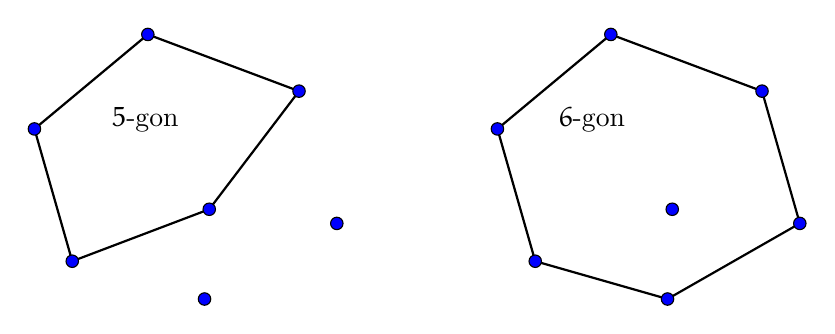
\begin{tikzpicture}[scale=1.5]
\newcommand\x{1.5}
  \draw[thick]
    (-.56, 3.48)
     -- (.40, 4.28)
     -- (1.68, 3.80)
     -- (.92, 2.80)
     -- (-.24, 2.36)
     -- (-.56, 3.48);
\vertex{-.56}{3.48}{\x};
\vertex{.40}{4.28}{\x};
\vertex{1.68}{3.80}{\x};
\vertex{2.00}{2.68}{\x};
\vertex{.88}{2.04}{\x};
\vertex{.92}{2.80}{\x};
\vertex{-.24}{2.36}{\x};
  \draw[thick]
    (3.68, 2.36)
     -- (3.36, 3.48)
     -- (4.32, 4.28)
     -- (5.60, 3.80)
     -- (5.92, 2.68)
     -- (4.80, 2.04)
     -- (3.68, 2.36);
\vertex{3.36}{3.48}{\x};
\vertex{4.32}{4.28}{\x};
\vertex{5.60}{3.80}{\x};
\vertex{5.92}{2.68}{\x};
\vertex{4.80}{2.04}{\x};
\vertex{4.84}{2.80}{\x};
\vertex{3.68}{2.36}{\x};
  \node
     at (.38, 3.56) {$5$-gon};
  \node
     at (4.16, 3.56) {$6$-gon};
\end{tikzpicture}
\end{center}

\begin{theorem}[Erd\H{o}s \& Szekeres 1935]
$\forall k \in \mathbb{N}, \exists$ a smallest integer $g(k)$ such that every set of $g(k)$ points contains a $k$-gon.
\end{theorem}

}

\frame{
	\frametitle{Bounds for Small $k$}

\large 

Clearly, it takes exactly three points in general position to have a $3$-gon (triangle)


\bigskip

Some sets of 4 points do not for a $4$-gon:

\bigskip

\centering

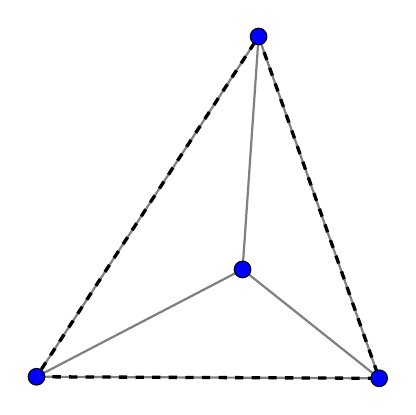
\begin{tikzpicture}[scale=1.5]
\newcommand{\x}{2}

  \draw [gray, thick] (0.423016, 4.503319) -- (2.303165, 7.383978);
  \draw [gray, thick] (0.423016, 4.503319) -- (3.32398, 4.490406);
  \draw [gray, thick] (0.423016, 4.503319) -- (2.167452, 5.411797);

  \draw [gray, thick] (3.32398, 4.490406) -- (2.303165, 7.383978);
  \draw [gray, thick] (2.167452, 5.411797) -- (3.32398, 4.490406);
  \draw [gray, thick] (2.303165, 7.383978) -- (2.167452, 5.411797);

  \draw[dashed, very thick]
    (2.30317, 7.38398)
     -- (3.32398, 4.490406)
     -- (0.42302, 4.503321)
     -- cycle;

\vertex{0.423016}{4.503319}{\x};
\vertex{2.303165}{7.383978}{\x};
\vertex{2.167452}{5.411797}{\x};
\vertex{3.32398}{4.490404}{\x};

\end{tikzpicture}

\bigskip

\pause



\structure{how many points imply a $4$-gon?}



}

\frame{
	\frametitle{Upperbound for $4$-Gon: $g(4) = 5$ \textcolor{xgreen}{[Klein]}}

\large

   \newcommand{\x}{0.75}


\centering
	
	
\begin{tikzpicture}[scale=2.5]

  \draw[shift={(1, 3.04)}, scale=1.5, thick]
    (0, 0)
     -- (0.64, 0.32)
     -- (1.12, 0)
     -- (0.8, -0.48)
     -- (0.32, -0.48)
     -- cycle;

\only<2->{
  \filldraw[shift={(1, 3.04)}, scale=1.5, draw=structure, very thick, fill=structure!30!white]
    (0, 0)
     -- (0.64, 0.32)
     -- (1.12, 0)
 %    -- (0.8, -0.48)
     -- (0.32, -0.48)
     -- cycle;     
}
     
  \vertex{2.2}{2.32}{\x};
  \vertex{2.68}{3.04}{\x};
  \vertex{1.96}{3.52}{\x};
  \vertex{1}{3.04}{\x};
  \vertex{1.48}{2.32}{\x};

\end{tikzpicture}
~~~~~~~~~~~~~~~~~~~~
\pause
\pause
\begin{tikzpicture}[scale=2.5]
  \draw[shift={(3.8, 2.32)}, scale=1.5, thick]
    (0, 0)
     -- (0, 0.8)
     -- (0.8, 0.64)
     -- (0.64, 0.16)
     -- cycle;

%  \draw[shift={(3.8, 3.52)}, scale=1.5]
%    (0, 0)
%     -- (0.64, -0.64);
%  \draw[shift={(3.8, 2.32)}, scale=1.5]
%    (0, 0)
%     -- (0.8, 0.64);

\only<4->{
  \filldraw[shift={(3.8, 2.32)}, scale=1.5, draw=structure, very thick, fill=structure!30!white]
    (0, 0)
     -- (0, 0.8)
     -- (0.8, 0.64)
     -- (0.64, 0.16)
     -- cycle;
%    (0, 0)
%     -- (0.16, -0.48)
%     -- (0.64, -0.64)
%     -- (0.8, -0.16)
%     -- cycle;
     
%   \draw[shift={(3.8, 3.52)}, scale=1.5]
%    (0, 0)
%     -- (0.64, -0.64);
%  \draw[shift={(3.8, 2.32)}, scale=1.5]
%    (0, 0)
%     -- (0.8, 0.64);
}

  \vertex{4.04}{2.8}{\x};
  \vertex{3.8}{3.52}{\x};
  \vertex{5}{3.28}{\x};
  \vertex{4.76}{2.56}{\x};
  \vertex{3.8}{2.32}{\x};

\end{tikzpicture}

\pause
\pause
	
\begin{tikzpicture}[scale=2.5]
     
  
    \draw[shift={(5.72, 2.56)}, scale=1.5]
    (0, 0)
     -- (1.28, 0.48);

  \draw[shift={(5.96, 2.32)}, scale=1.5, thick]
    (0, 0)
     -- (0.48, 0.96)
     -- (0.96, 0.16)
     -- cycle;

\only<6->{

    \draw[shift={(5.72, 2.56)}, scale=1.5]
    (0, 0)
     -- (1.28, 0.48);
     
  \filldraw[shift={(5.96, 2.32)}, scale=1.5, draw=structure, very thick, fill=structure!30!white]
    (0, 0)
     -- (0.3426, 0.348475)
     -- (0.59104, 0.44164)
     -- (0.96, 0.16)
     -- cycle;
 }
 
  \vertex{6.4739}{2.842713}{\x};
  \vertex{6.84656}{2.98246}{\x};
  \vertex{5.96}{2.32}{\x};
  \vertex{6.68}{3.76}{\x};
  \vertex{7.4}{2.56}{\x};
  

  \end{tikzpicture}	

}

\frame{
	\frametitle{Bound Results for $5$-Gon and $6$-Gon}


\begin{minipage}{0.45\textwidth}
$g(5) = 9$
\begin{itemize}
\item \textcolor{xgreen}{[Kalbfleisch \& Stanton '70]}
\end{itemize}
\end{minipage}
\begin{minipage}{0.45\textwidth}
\centering
\medskip
~~~~~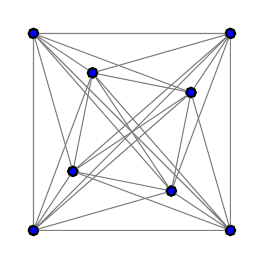
\begin{tikzpicture}[scale=0.5]

\node[draw,circle, thick, fill=blue, scale=0.3] (a) at (0,0) {};
\node[draw,circle, thick, fill=blue, scale=0.3] (b) at (5,0) {};
\node[draw,circle, thick, fill=blue, scale=0.3] (c) at (0,5) {};
\node[draw,circle, thick, fill=blue, scale=0.3] (d) at (5,5) {};

\node[draw,circle, thick, fill=blue, scale=0.3] (e) at (1,1.5) {};
\node[draw,circle, thick, fill=blue, scale=0.3] (f) at (3.5,1) {};
\node[draw,circle, thick, fill=blue, scale=0.3] (g) at (1.5,4) {};
\node[draw,circle, thick, fill=blue, scale=0.3] (h) at (4,3.5) {};

\draw[gray] (a) -- (b) (a) -- (c) (a) -- (d) (a) -- (e) (a) -- (f) (a) -- (g) (a) -- (h);
\draw[gray] (b) -- (c) (b) -- (d) (b) -- (e) (b) -- (f) (b) -- (g) (b) -- (h);
\draw[gray] (c) -- (d) (c) -- (e) (c) -- (f) (c) -- (g) (c) -- (h);
\draw[gray] (d) -- (e) (d) -- (f) (d) -- (g) (d) -- (h);
\draw[gray] (e) -- (f) (e) -- (g) (e) -- (h);
\draw[gray] (f) -- (g) (f) -- (h)  (g) -- (h);
 
\end{tikzpicture}
\end{minipage}


\begin{minipage}{0.45\textwidth}
\centering
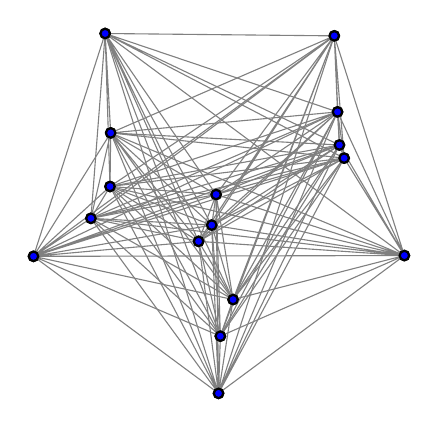
\begin{tikzpicture}[scale=1]

\node[draw,circle, thick, fill=blue, scale=0.3] (a) at (0.19, 1.95) {};
\node[draw,circle, thick, fill=blue, scale=0.3] (b) at (2.54, 0.21) {};
\node[draw,circle, thick, fill=blue, scale=0.3] (c) at (4.9, 1.96) {};
\node[draw,circle, thick, fill=blue, scale=0.3] (d) at (4.01, 4.75) {};
\node[draw,circle, thick, fill=blue, scale=0.3] (e) at (1.1, 4.78) {};
\node[draw,circle, thick, fill=blue, scale=0.3] (f) at (2.5091, 2.735) {};
\node[draw,circle, thick, fill=blue, scale=0.3] (g) at (1.1702, 3.5174) {};
\node[draw,circle, thick, fill=blue, scale=0.3] (h) at (4.0512, 3.7842) {};
\node[draw,circle, thick, fill=blue, scale=0.3] (i) at (2.7243, 1.4014) {};
\node[draw,circle, thick, fill=blue, scale=0.3] (j) at (0.9192, 2.4327) {};
\node[draw,circle, thick, fill=blue, scale=0.3] (k) at (4.1349, 3.1973) {};
\node[draw,circle, thick, fill=blue, scale=0.3] (l) at (2.2864, 2.1402) {};
\node[draw,circle, thick, fill=blue, scale=0.3] (m) at (2.5628, 0.9363) {};
\node[draw,circle, thick, fill=blue, scale=0.3] (n) at (1.1617, 2.8371) {};
\node[draw,circle, thick, fill=blue, scale=0.3] (o) at (2.4537, 2.3468) {};
\node[draw,circle, thick, fill=blue, scale=0.3] (p) at (4.0752, 3.364) {};
 
 
\draw[gray] (a) -- (b) (a) -- (c) (a) -- (d) (a) -- (e) (a) -- (f) (a) -- (g) (a) -- (h) (a) -- (i) (a) -- (j) (a) -- (k) (a) -- (l) (a) -- (m) (a) -- (n) (a) -- (o) (a) -- (p);
\draw[gray] (b) -- (c) (b) -- (d) (b) -- (e) (b) -- (f) (b) -- (g) (b) -- (h) (b) -- (i) (b) -- (j) (b) -- (k) (b) -- (l) (b) -- (m) (b) -- (n) (b) -- (o) (b) -- (p);
\draw[gray] (c) -- (d) (c) -- (e) (c) -- (f) (c) -- (g) (c) -- (h) (c) -- (i) (c) -- (j) (c) -- (k) (c) -- (l) (c) -- (m) (c) -- (n) (c) -- (o) (c) -- (p);
\draw[gray] (d) -- (e) (d) -- (f) (d) -- (g) (d) -- (h) (d) -- (i) (d) -- (j) (d) -- (k) (d) -- (l) (d) -- (m) (d) -- (n) (d) -- (o) (d) -- (p);
\draw[gray] (e) -- (f) (e) -- (g) (e) -- (h) (e) -- (i) (e) -- (j) (e) -- (k) (e) -- (l) (e) -- (m) (e) -- (n) (e) -- (o) (e) -- (p);
\draw[gray] (f) -- (g) (f) -- (h) (f) -- (i) (f) -- (j) (f) -- (k) (f) -- (l) (f) -- (m) (f) -- (n) (f) -- (o) (f) -- (p);
\draw[gray] (g) -- (h) (g) -- (i) (g) -- (j) (g) -- (k) (g) -- (l) (g) -- (m) (g) -- (n) (g) -- (o) (g) -- (p);
\draw[gray] (h) -- (i) (h) -- (j) (h) -- (k) (h) -- (l) (h) -- (m) (h) -- (n) (h) -- (o) (h) -- (p);
\draw[gray] (i) -- (j) (i) -- (k) (i) -- (l) (i) -- (m) (i) -- (n) (i) -- (o) (i) -- (p);
\draw[gray] (j) -- (k) (j) -- (l) (j) -- (m) (j) -- (n) (j) -- (o) (j) -- (p);
\draw[gray] (k) -- (l) (k) -- (m) (k) -- (n) (k) -- (o) (k) -- (p);
\draw[gray] (l) -- (m) (l) -- (n) (l) -- (o) (l) -- (p);
\draw[gray] (m) -- (n) (m) -- (o) (m) -- (p);
\draw[gray] (n) -- (o) (n) -- (p) (o) -- (p); 
 
 \node[draw,circle, thick, fill=blue, scale=0.3] (a) at (0.19, 1.95) {};
\node[draw,circle, thick, fill=blue, scale=0.3] (b) at (2.54, 0.21) {};
\node[draw,circle, thick, fill=blue, scale=0.3] (c) at (4.9, 1.96) {};
\node[draw,circle, thick, fill=blue, scale=0.3] (d) at (4.01, 4.75) {};
\node[draw,circle, thick, fill=blue, scale=0.3] (e) at (1.1, 4.78) {};
\node[draw,circle, thick, fill=blue, scale=0.3] (f) at (2.5091, 2.735) {};
\node[draw,circle, thick, fill=blue, scale=0.3] (g) at (1.1702, 3.5174) {};
\node[draw,circle, thick, fill=blue, scale=0.3] (h) at (4.0512, 3.7842) {};
\node[draw,circle, thick, fill=blue, scale=0.3] (i) at (2.7243, 1.4014) {};
\node[draw,circle, thick, fill=blue, scale=0.3] (j) at (0.9192, 2.4327) {};
\node[draw,circle, thick, fill=blue, scale=0.3] (k) at (4.1349, 3.1973) {};
\node[draw,circle, thick, fill=blue, scale=0.3] (l) at (2.2864, 2.1402) {};
\node[draw,circle, thick, fill=blue, scale=0.3] (m) at (2.5628, 0.9363) {};
\node[draw,circle, thick, fill=blue, scale=0.3] (n) at (1.1617, 2.8371) {};
\node[draw,circle, thick, fill=blue, scale=0.3] (o) at (2.4537, 2.3468) {};
\node[draw,circle, thick, fill=blue, scale=0.3] (p) at (4.0752, 3.364) {};
 
\end{tikzpicture}
\end{minipage}
~~~
\begin{minipage}{0.45\textwidth}
$g(6) = 17$
\begin{itemize}
\item Computer-assisted proof, 1500 CPU hours \textcolor{xgreen}{[SzekeresPeters '06]}
\item One CPU hour using a SAT solver \textcolor{xgreen}{[Scheucher '18]}
\item $20$ seconds using new encoding\!\!\!\!\!\!\!\!\!\!\!\!
\end{itemize}
\end{minipage}

}


\frame{
	\frametitle{Bound History}

\large

\begin{theorem}[\textcolor{xgreen}{Erd\H{o}s \& Szekeres '35, '60}]
$2^{k-2} +1 \leq g(k) \leq \binom{2k-4}{k-2}+1$~~~~~($\mathrm{of~magnitude}$ $4^{k-o(k)}$)
\end{theorem}

\begin{itemize}
\item Equality with lower bound conjectured by Szekeres
\item Erd\H{o}s offered \$500 for a proof
\end{itemize}

\bigskip

\begin{theorem}[\textcolor{xgreen}{Suk ’16}]
$g(k) \leq 2^{k+o(k)}$ 
\end{theorem}

\bigskip

\begin{theorem}[\textcolor{xgreen}{Holmsen, Mojarrad, Pach, and Tardos ’17}]
$g(k) \leq 2^{k+O(\sqrt{k log k})}$
\end{theorem}	

}

\frame{
	\frametitle{$k$-Holes}
	
\large

A \structure{$k$-hole} (in $S$) is the vertex set of a convex $k$-gon
containing no other points of $S$. We denote with \structure{$h(k)$} the smallest number of points that contain a $k$-hole.

\bigskip

Erd\H{o}s, 1970’s: For $k$ fixed, does every sufficiently large
point set contain $k$-holes?

\bigskip
\bigskip
\centering

\begin{tikzpicture}[scale=1.5]
\newcommand\x{1}
  \filldraw[thick, draw=xgreen, fill=xgreen!30!white]
    (-.56, 3.48)
     -- (.40, 4.28)
     -- (1.68, 3.80)
     -- (.92, 2.80)
     -- (-.24, 2.36)
     -- (-.56, 3.48);
\vertex{-.56}{3.48}{\x};
\vertex{.40}{4.28}{\x};
\vertex{1.68}{3.80}{\x};
\vertex{2.00}{2.68}{\x};
\vertex{.88}{2.04}{\x};
\vertex{.92}{2.80}{\x};
\vertex{-.24}{2.36}{\x};
  \filldraw[thick, draw=structure, fill=structure!30!white]
    (3.68, 2.36)
     -- (3.36, 3.48)
     -- (4.32, 4.28)
     -- (5.60, 3.80)
     -- (5.92, 2.68)
     -- (4.80, 2.04)
     -- (3.68, 2.36);
\vertex{3.36}{3.48}{\x};
\vertex{4.32}{4.28}{\x};
\vertex{5.60}{3.80}{\x};
\vertex{5.92}{2.68}{\x};
\vertex{4.80}{2.04}{\x};
\vertex{4.84}{2.80}{\x};
\vertex{3.68}{2.36}{\x};
  \node
     at (.38, 3.56) {$5$-hole};
  \node
     at (4.46, 3.56) {not a $6$-hole};
\end{tikzpicture}

}

\frame{
	\frametitle{$k$-Holes Overview}

\large

A \structure{$k$-hole} (in $S$) is the vertex set of a convex $k$-gon
containing no other points of $S$

\bigskip

Erd\H{o}s, 1970’s: For $k$ fixed, does every \structure{sufficiently large}
point set contain $k$-holes?
\begin{itemize}
\item $3$ points $\Rightarrow \exists$ $3$-hole
\item $5$ points $\Rightarrow \exists$ $4$-hole
\item $10$ points $\Rightarrow \exists$ $5$-hole \textcolor{xgreen}{[Harborth ’78]}
\item Arbitrarily large point sets with no $7$-hole  \textcolor{xgreen}{[Horton ’83]}
\end{itemize}

\bigskip

Main open question: what about $6$-hole?
\begin{itemize}
\item Sufficiently large point sets contain a $6$-hole\\
\textcolor{xgreen}{[Gerken ’08 and Nicol\'as ’07, independently]}
\item \structure{Conjecture}: $h(6) = 30$
\end{itemize}

}

\section{$k$-Hole Results}
\frame{\Large \tableofcontents[currentsection]}

\frame{
	\frametitle{Lowerbound for $4$-Hole: $h(4) > 4$}
	
	\large
	
	Same example as $g(4) > 4$:
	
	\bigskip
	\centering
	
	
	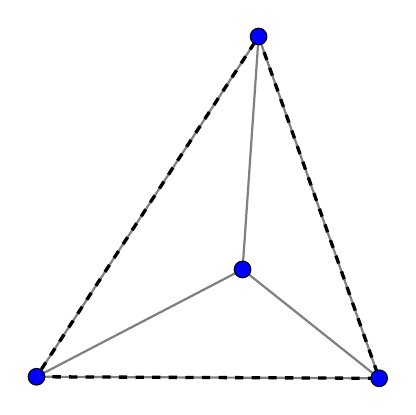
\begin{tikzpicture}[scale=1.5]
\newcommand{\x}{2}

  \draw [gray, thick] (0.423016, 4.503319) -- (2.303165, 7.383978);
  \draw [gray, thick] (0.423016, 4.503319) -- (3.32398, 4.490406);
  \draw [gray, thick] (0.423016, 4.503319) -- (2.167452, 5.411797);

  \draw [gray, thick] (3.32398, 4.490406) -- (2.303165, 7.383978);
  \draw [gray, thick] (2.167452, 5.411797) -- (3.32398, 4.490406);
  \draw [gray, thick] (2.303165, 7.383978) -- (2.167452, 5.411797);

  \draw[dashed, very thick]
    (2.30317, 7.38398)
     -- (3.32398, 4.490406)
     -- (0.42302, 4.503321)
     -- cycle;

\vertex{0.423016}{4.503319}{\x};
\vertex{2.303165}{7.383978}{\x};
\vertex{2.167452}{5.411797}{\x};
\vertex{3.32398}{4.490404}{\x};

\end{tikzpicture}
	
}

\frame{
	\frametitle{Upperbound for $4$-Hole: $h(4) = 5$}

\large

   \newcommand{\x}{0.75}


\centering
	
	
\begin{tikzpicture}[scale=2.5]

  \draw[shift={(1, 3.04)}, scale=1.5, thick]
    (0, 0)
     -- (0.64, 0.32)
     -- (1.12, 0)
     -- (0.8, -0.48)
     -- (0.32, -0.48)
     -- cycle;

\only<2->{
  \filldraw[shift={(1, 3.04)}, scale=1.5, draw=structure, very thick, fill=structure!30!white]
    (0, 0)
     -- (0.64, 0.32)
     -- (1.12, 0)
 %    -- (0.8, -0.48)
     -- (0.32, -0.48)
     -- cycle;     
}
     
  \vertex{2.2}{2.32}{\x};
  \vertex{2.68}{3.04}{\x};
  \vertex{1.96}{3.52}{\x};
  \vertex{1}{3.04}{\x};
  \vertex{1.48}{2.32}{\x};

\end{tikzpicture}
~~~~~~~~~~~~~~~~~~~~
\pause
\pause
\begin{tikzpicture}[scale=2.5]
  \draw[shift={(3.8, 2.32)}, scale=1.5, thick]
    (0, 0)
     -- (0, 0.8)
     -- (0.8, 0.64)
     -- (0.64, 0.16)
     -- cycle;

  \draw[shift={(3.8, 3.52)}, scale=1.5]
    (0, 0)
     -- (0.64, -0.64);
  \draw[shift={(3.8, 2.32)}, scale=1.5]
    (0, 0)
     -- (0.8, 0.64);

\only<4->{
  \filldraw[shift={(3.8, 3.52)}, scale=1.5, draw=structure, very thick, fill=structure!30!white]
    (0, 0)
     -- (0.16, -0.48)
     -- (0.64, -0.64)
     -- (0.8, -0.16)
     -- cycle;
     
   \draw[shift={(3.8, 3.52)}, scale=1.5]
    (0, 0)
     -- (0.64, -0.64);
  \draw[shift={(3.8, 2.32)}, scale=1.5]
    (0, 0)
     -- (0.8, 0.64);
}

  \vertex{4.04}{2.8}{\x};
  \vertex{3.8}{3.52}{\x};
  \vertex{5}{3.28}{\x};
  \vertex{4.76}{2.56}{\x};
  \vertex{3.8}{2.32}{\x};

\end{tikzpicture}

\pause
\pause
	
\begin{tikzpicture}[scale=2.5]
     
  
    \draw[shift={(5.72, 2.56)}, scale=1.5]
    (0, 0)
     -- (1.28, 0.48);

  \draw[shift={(5.96, 2.32)}, scale=1.5, thick]
    (0, 0)
     -- (0.48, 0.96)
     -- (0.96, 0.16)
     -- cycle;

\only<6->{

    \draw[shift={(5.72, 2.56)}, scale=1.5]
    (0, 0)
     -- (1.28, 0.48);
     
  \filldraw[shift={(5.96, 2.32)}, scale=1.5, draw=structure, very thick, fill=structure!30!white]
    (0, 0)
     -- (0.3426, 0.348475)
     -- (0.59104, 0.44164)
     -- (0.96, 0.16)
     -- cycle;
 }
 
  \vertex{6.4739}{2.842713}{\x};
  \vertex{6.84656}{2.98246}{\x};
  \vertex{5.96}{2.32}{\x};
  \vertex{6.68}{3.76}{\x};
  \vertex{7.4}{2.56}{\x};
  

  \end{tikzpicture}
	
}

\frame{
	\frametitle{Lowerbound for $5$-Hole: $h(5) \geq 10$}

\large

\begin{center}
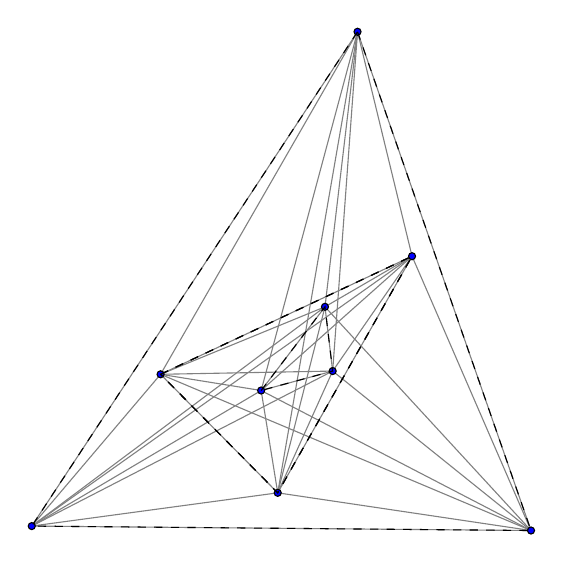
\begin{tikzpicture}[scale=1.7]
\newcommand{\x}{0.75}
\draw[shift={(1.26017, 1.37339)}, rotate=-89.8437, scale=0.63, gray]
  (0, 0)
   -- (-5.85132, 3.87897);
\draw[shift={(1.26017, 1.37339)}, rotate=-89.8437, scale=0.63, gray]
  (0, 0)
   -- (-3.18788, 4.5182);
\draw[shift={(1.26017, 1.37339)}, rotate=-89.8437, scale=0.63, gray]
  (0, 0)
   -- (-1.79574, 1.53246);
\draw[shift={(1.26017, 1.37339)}, rotate=-89.8437, scale=0.63, gray]
  (0, 0)
   -- (-2.59075, 3.48411);
\draw[shift={(1.26017, 1.37339)}, rotate=-89.8437, scale=0.63, gray]
  (0, 0)
   -- (-1.60036, 2.7245);
\draw[shift={(1.26017, 1.37339)}, rotate=-89.8437, scale=0.63, gray]
  (0, 0)
   -- (-1.82854, 3.57324);
\draw[shift={(1.26017, 1.37339)}, rotate=-89.8437, scale=0.63, gray]
  (0, 0)
   -- (-0.38641, 2.91774);
\draw[shift={(1.26017, 1.37339)}, rotate=-89.8437, scale=0.63, gray]
  (0, 0)
   -- (0.06868, 5.92);
\draw[shift={(3.69386, 5.06637)}, rotate=-89.8437, scale=0.63, gray]
  (0, 0)
   -- (2.66344, 0.63923);
\draw[shift={(3.69386, 5.06637)}, rotate=-89.8437, scale=0.63, gray]
  (0, 0)
   -- (4.05558, -2.34651);
\draw[shift={(3.69386, 5.06637)}, rotate=-89.8437, scale=0.63, gray]
  (0, 0)
   -- (3.26057, -0.39486);
\draw[shift={(3.69386, 5.06637)}, rotate=-89.8437, scale=0.63, gray]
  (0, 0)
   -- (4.25096, -1.15447);
\draw[shift={(3.69386, 5.06637)}, rotate=-89.8437, scale=0.63, gray]
  (0, 0)
   -- (4.02278, -0.30573);
\draw[shift={(3.69386, 5.06637)}, rotate=-89.8437, scale=0.63, gray]
  (0, 0)
   -- (5.46491, -0.96123);
\draw[shift={(3.69386, 5.06637)}, rotate=-89.8437, scale=0.63, gray]
  (0, 0)
   -- (5.92, 2.04103);
\draw[shift={(4.10115, 3.38951)}, rotate=-89.8437, scale=0.63, gray]
  (0, 0)
   -- (1.39214, -2.98574);
\draw[shift={(4.10115, 3.38951)}, rotate=-89.8437, scale=0.63, gray]
  (0, 0)
   -- (0.59713, -1.03409);
\draw[shift={(4.10115, 3.38951)}, rotate=-89.8437, scale=0.63, gray]
  (0, 0)
   -- (1.58752, -1.7937);
\draw[shift={(4.10115, 3.38951)}, rotate=-89.8437, scale=0.63, gray]
  (0, 0)
   -- (1.35934, -0.94496);
\draw[shift={(4.10115, 3.38951)}, rotate=-89.8437, scale=0.63, gray]
  (0, 0)
   -- (2.80147, -1.60046);
\draw[shift={(4.10115, 3.38951)}, rotate=-89.8437, scale=0.63, gray]
  (0, 0)
   -- (3.25656, 1.4018);
\draw[shift={(2.22253, 2.50734)}, rotate=-89.8437, scale=0.63, gray]
  (0, 0)
   -- (-0.79501, 1.95165);
\draw[shift={(2.22253, 2.50734)}, rotate=-89.8437, scale=0.63, gray]
  (0, 0)
   -- (0.19538, 1.19204);
\draw[shift={(2.22253, 2.50734)}, rotate=-89.8437, scale=0.63, gray]
  (0, 0)
   -- (-0.0328, 2.04078);
\draw[shift={(2.22253, 2.50734)}, rotate=-89.8437, scale=0.63, gray]
  (0, 0)
   -- (1.40933, 1.38528);
\draw[shift={(2.22253, 2.50734)}, rotate=-89.8437, scale=0.63, gray]
  (0, 0)
   -- (1.86442, 4.38754);
\draw[shift={(3.4507, 3.01154)}, rotate=-89.8437, scale=0.63, gray]
  (0, 0)
   -- (0.99039, -0.75961);
\draw[shift={(3.4507, 3.01154)}, rotate=-89.8437, scale=0.63, gray]
  (0, 0)
   -- (0.76221, 0.08913);
\draw[shift={(3.4507, 3.01154)}, rotate=-89.8437, scale=0.63, gray]
  (0, 0)
   -- (2.20434, -0.56637);
\draw[shift={(3.4507, 3.01154)}, rotate=-89.8437, scale=0.63, gray]
  (0, 0)
   -- (2.65943, 2.43589);
\draw[shift={(2.97385, 2.38629)}, rotate=-89.8437, scale=0.63, gray]
  (0, 0)
   -- (-0.22818, 0.84874);
\draw[shift={(2.97385, 2.38629)}, rotate=-89.8437, scale=0.63, gray]
  (0, 0)
   -- (1.21395, 0.19324);
\draw[shift={(2.97385, 2.38629)}, rotate=-89.8437, scale=0.63, gray]
  (0, 0)
   -- (1.66904, 3.1955);
\draw[shift={(3.50817, 2.53151)}, rotate=-89.8437, scale=0.63, gray]
  (0, 0)
   -- (1.44213, -0.6555);
\draw[shift={(3.50817, 2.53151)}, rotate=-89.8437, scale=0.63, gray]
  (0, 0)
   -- (1.89722, 2.34676);
\draw[shift={(3.09768, 1.62184)}, rotate=-89.8437, scale=0.63, gray]
  (0, 0)
   -- (0.45509, 3.00226);
\vertex{1.26017}{1.37339}{\x};
\vertex{3.69386}{5.06637}{\x};
\vertex{4.10115}{3.38951}{\x};
\vertex{2.22253}{2.50734}{\x};
\vertex{3.4507}{3.01154}{\x};
\vertex{2.97385}{2.38629}{\x};
\vertex{3.50817}{2.53151}{\x};
\vertex{3.09768}{1.62184}{\x};
\vertex{4.98988}{1.34029}{\x};
\draw[dashed]
  (3.69386, 5.06637)
   -- (4.98988, 1.34029)
   -- (1.26017, 1.37339)
   -- cycle;
\draw[dashed]
  (2.22254, 2.50733)
   -- (4.10115, 3.38951)
   -- (3.09768, 1.62184)
   -- cycle;
\draw[dashed]
  (2.22254, 2.50733)
   -- (4.10115, 3.38951)
   -- (3.09768, 1.62184)
   -- cycle;
\draw[dashed]
  (2.97385, 2.38629)
   -- (3.4507, 3.01154)
   -- (3.50817, 2.53151)
   -- cycle;
\end{tikzpicture}
\end{center}

All 5-gons in these 9 points have an inner point: $h(5) = 10$
	
}

\frame{
	\frametitle{Lowerbound for $6$-Hole: $h(6) \geq 30$}

\large

\begin{center}
	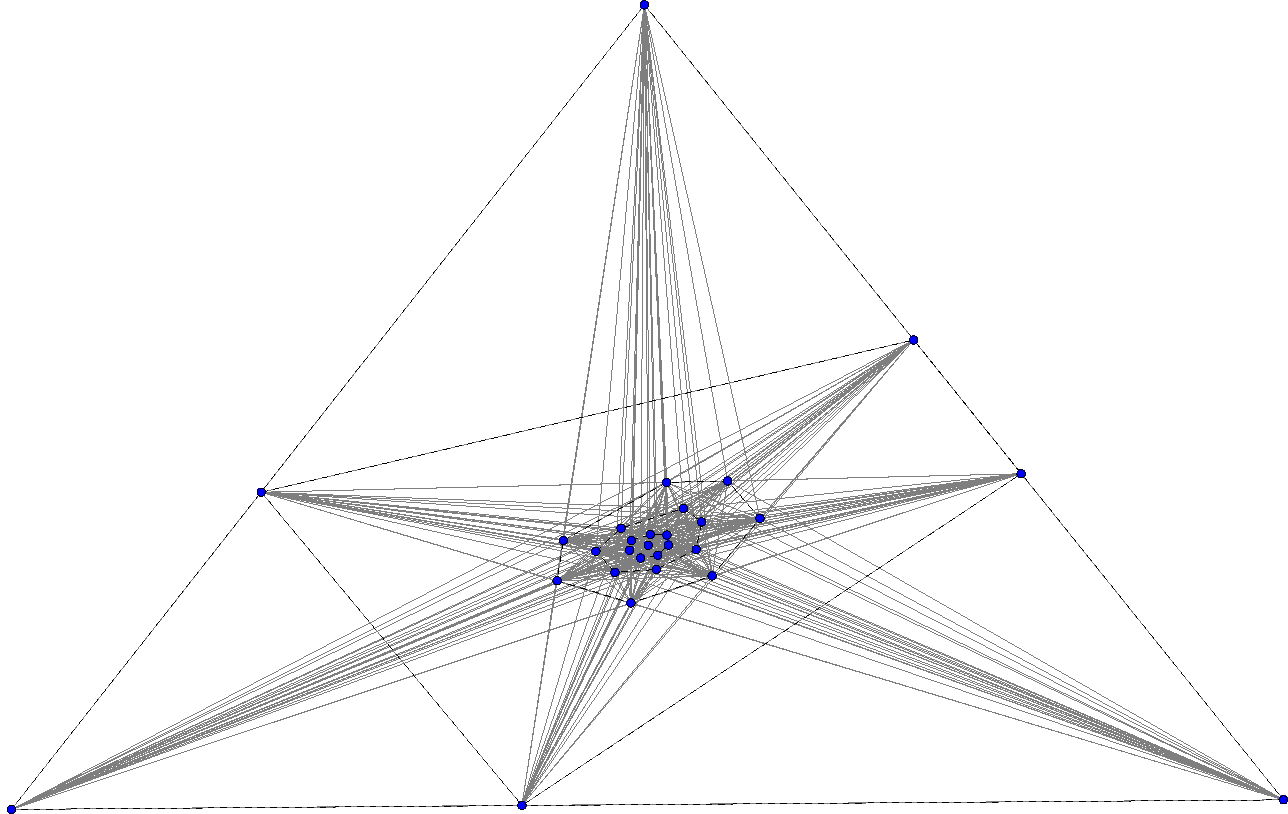
\includegraphics[width=.75\textwidth]{lb6hole.pdf}
\end{center}

29 points, no $6$-hole \textcolor{xgreen}{[Overmars ’02]}
\begin{itemize}
\item Found using simulated annealing... is now \structure{easy using SAT}
\item This contains $7$-gon. Each $9$-gon contains a $6$-hole
\end{itemize}

}

\frame{
	\frametitle{No Lowerbound for $7$-Hole: Horton's Construction (I)}


\bigskip
\bigskip

\begin{minipage}{.45\textwidth}
\centering

\begin{tikzpicture}[scale=1.5]

\node[draw,circle, fill=blue, scale=0.3] (a) at (2.786402,4.8952) {};
\node[draw,circle, fill=structure, scale=0.3] (b) at (0.6552,4.8952) {};


\draw[gray] (a) -- (b) ;


 
\end{tikzpicture}

\bigskip

$2^1$ points, no 7-hole

\bigskip
\bigskip
\bigskip

\pause

\begin{tikzpicture}[scale=1.5]

\node[draw,circle, fill=structure, scale=0.3] (a) at (2.786402,4.8952) {};
\node[draw,circle, fill=blue, scale=0.3] (c) at (3.852003,5.8276) {};
\node[draw,circle, fill=structure, scale=0.3] (b) at (0.6552,4.8952) {};
\node[draw,circle, fill=blue, scale=0.3] (d) at (1.720801,5.8276) {};


\draw[structure, thick] (a) -- (b) ;
\draw[gray] (a) -- (c) (a) -- (d) (b) -- (c) (b) -- (d) ; 
\draw[blue, thick] (c) -- (d); 

 
\end{tikzpicture}

\bigskip

$2^2$ points, no 7-hole

\end{minipage}
~~~\pause
\begin{minipage}{.45\textwidth}
\centering
\begin{tikzpicture}[scale=1.5]

\node[draw,circle, fill=structure, scale=0.3] (a) at (2.786402,4.8952) {};
\node[draw,circle, fill=structure, scale=0.3] (b) at (3.852003,5.8276) {};
\node[draw,circle, fill=structure, scale=0.3] (c) at (0.6552,4.8952) {};
\node[draw,circle, fill=structure, scale=0.3] (d) at (1.720801,5.8276) {};

\node[draw,circle, fill=blue, scale=0.3] (e) at (1.188,7.6924) {};
\node[draw,circle, fill=blue, scale=0.3] (f) at (3.319199,7.6924) {};
\node[draw,circle, fill=blue, scale=0.3] (g) at (2.253598,8.6248) {};
\node[draw,circle, fill=blue, scale=0.3] (h) at (4.3848,8.6248) {};

\draw[structure, thick] (a) -- (b) (a) -- (c) (a) -- (d) (c) -- (d) (b) -- (c) (b) -- (d);
\draw[gray]  (a) -- (e) (a) -- (f) (a) -- (g) (a) -- (h) (b) -- (e) (b) -- (f) (b) -- (g) (b) -- (h);
\draw[gray] (c) -- (d)  (c) -- (e) (c) -- (f) (c) -- (g) (c) -- (h);
\draw[gray] (d) -- (e) (d) -- (f) (d) -- (g) (d) -- (h);
\draw[blue, thick] (e) -- (f) (e) -- (g) (e) -- (h);
\draw[blue, thick] (f) -- (g) (f) -- (h)  (g) -- (h);


 
\end{tikzpicture}

\bigskip

$2^3$ points, no 7-hole
\end{minipage}
	
}

\iffalse
\frame{
	\frametitle{No Lowerbound for $7$-Hole: Horton's Construction (II)}

\centering

\begin{tikzpicture}[scale=1.7]

\node[draw,circle, fill=structure, scale=0.3] (a) at (0.6552, 5.1752) {};
\node[draw,circle, fill=structure, scale=0.3] (b) at (2.644318, 5.1752) {};
\node[draw,circle, fill=structure, scale=0.3] (c) at (1.649762, 5.29175) {};
\node[draw,circle, fill=structure, scale=0.3] (d) at (3.63888, 5.29175) {};
\node[draw,circle, fill=structure, scale=0.3] (e) at (1.15248, 5.52485) {};
\node[draw,circle, fill=structure, scale=0.3] (f) at (3.141602, 5.52485) {};
\node[draw,circle, fill=structure, scale=0.3] (g) at (2.14704, 5.6414) {};
\node[draw,circle, fill=structure, scale=0.3] (h) at (4.136158, 5.6414) {};
\node[draw,circle, fill=blue, scale=0.3] (i) at (0.90384, 8.4386) {};
\node[draw,circle, fill=blue, scale=0.3] (j) at (2.89296, 8.4386) {};
\node[draw,circle, fill=blue, scale=0.3] (k) at (1.898398, 8.55515) {};
\node[draw,circle, fill=blue, scale=0.3] (l) at (3.887522, 8.55515) {};
\node[draw,circle, fill=blue, scale=0.3] (m) at (1.40112, 8.78825) {};
\node[draw,circle, fill=blue, scale=0.3] (n) at (3.390238, 8.78825) {};
\node[draw,circle, fill=blue, scale=0.3] (o) at (2.395682, 8.9048) {};
\node[draw,circle, fill=blue, scale=0.3] (p) at (4.3848, 8.9048) {};
 
 
\draw[structure,thick] (a) -- (b) (a) -- (c) (a) -- (d) (a) -- (e) (a) -- (f) (a) -- (g) (a) -- (h);
\draw[structure,thick] (b) -- (c) (b) -- (d) (b) -- (e) (b) -- (f) (b) -- (g) (b) -- (h);
\draw[structure,thick] (c) -- (d) (c) -- (e) (c) -- (f) (c) -- (g) (c) -- (h);
\draw[structure,thick] (d) -- (e) (d) -- (f) (d) -- (g) (d) -- (h); 
\draw[structure,thick] (e) -- (f) (e) -- (g) (e) -- (h) ;
\draw[structure,thick] (f) -- (g) (f) -- (h) ;
\draw[structure,thick] (g) -- (h) ;
\draw[gray] (a) -- (i) (a) -- (j) (a) -- (k) (a) -- (l) (a) -- (m) (a) -- (n) (a) -- (o) (a) -- (p);
\draw[gray] (b) -- (i) (b) -- (j) (b) -- (k) (b) -- (l) (b) -- (m) (b) -- (n) (b) -- (o) (b) -- (p);
\draw[gray] (c) -- (i) (c) -- (j) (c) -- (k) (c) -- (l) (c) -- (m) (c) -- (n) (c) -- (o) (c) -- (p);
\draw[gray] (d) -- (i) (d) -- (j) (d) -- (k) (d) -- (l) (d) -- (m) (d) -- (n) (d) -- (o) (d) -- (p);
\draw[gray] (e) -- (i) (e) -- (j) (e) -- (k) (e) -- (l) (e) -- (m) (e) -- (n) (e) -- (o) (e) -- (p);
\draw[gray] (f) -- (i) (f) -- (j) (f) -- (k) (f) -- (l) (f) -- (m) (f) -- (n) (f) -- (o) (f) -- (p);
\draw[gray] (g) -- (i) (g) -- (j) (g) -- (k) (g) -- (l) (g) -- (m) (g) -- (n) (g) -- (o) (g) -- (p);
 \draw[gray] (h) -- (i) (h) -- (j) (h) -- (k) (h) -- (l) (h) -- (m) (h) -- (n) (h) -- (o) (h) -- (p);
\draw[blue,thick] (i) -- (j) (i) -- (k) (i) -- (l) (i) -- (m) (i) -- (n) (i) -- (o) (i) -- (p);
\draw[blue,thick] (j) -- (k) (j) -- (l) (j) -- (m) (j) -- (n) (j) -- (o) (j) -- (p);
\draw[blue,thick] (k) -- (l) (k) -- (m) (k) -- (n) (k) -- (o) (k) -- (p);
\draw[blue,thick] (l) -- (m) (l) -- (n) (l) -- (o) (l) -- (p);
\draw[blue,thick] (m) -- (n) (m) -- (o) (m) -- (p);
\draw[blue,thick] (n) -- (o) (n) -- (p) (o) -- (p);
 
 \node[draw,circle, fill=structure, scale=0.3] (a) at (0.6552, 5.1752) {};
\node[draw,circle, fill=structure, scale=0.3] (b) at (2.644318, 5.1752) {};
\node[draw,circle, fill=structure, scale=0.3] (c) at (1.649762, 5.29175) {};
\node[draw,circle, fill=structure, scale=0.3] (d) at (3.63888, 5.29175) {};
\node[draw,circle, fill=structure, scale=0.3] (e) at (1.15248, 5.52485) {};
\node[draw,circle, fill=structure, scale=0.3] (f) at (3.141602, 5.52485) {};
\node[draw,circle, fill=structure, scale=0.3] (g) at (2.14704, 5.6414) {};
\node[draw,circle, fill=structure, scale=0.3] (h) at (4.136158, 5.6414) {};
\node[draw,circle, fill=blue, scale=0.3] (i) at (0.90384, 8.4386) {};
\node[draw,circle, fill=blue, scale=0.3] (j) at (2.89296, 8.4386) {};
\node[draw,circle, fill=blue, scale=0.3] (k) at (1.898398, 8.55515) {};
\node[draw,circle, fill=blue, scale=0.3] (l) at (3.887522, 8.55515) {};
\node[draw,circle, fill=blue, scale=0.3] (m) at (1.40112, 8.78825) {};
\node[draw,circle, fill=blue, scale=0.3] (n) at (3.390238, 8.78825) {};
\node[draw,circle, fill=blue, scale=0.3] (o) at (2.395682, 8.9048) {};
\node[draw,circle, fill=blue, scale=0.3] (p) at (4.3848, 8.9048) {};
 
  
\end{tikzpicture}

\bigskip

 $2^4$ points, no 7-hole


}
\fi

\frame{
	\frametitle{No Lowerbound for $7$-Hole: Horton's Construction (III)}
	
	\centering
	
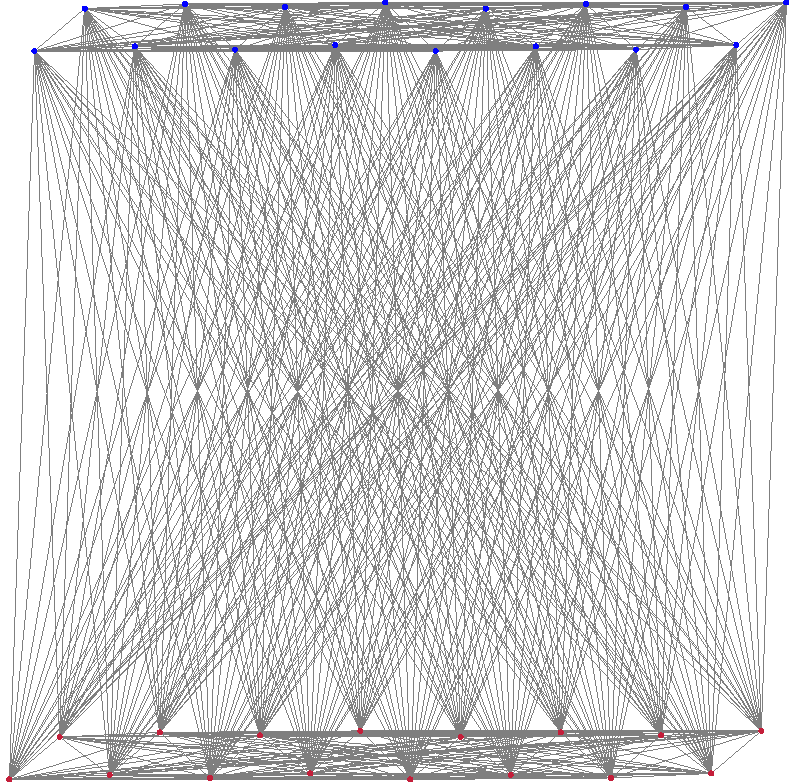
\includegraphics[height=180pt]{7hole-final.pdf}
	
	\bigskip
	
	 $2^5$ points, no 7-hole

}


\section{SAT Encoding}
\frame{\Large \tableofcontents[currentsection]}


\frame{
	\frametitle{Orientation Variables}
	
\large 
\begin{minipage}{.62\textwidth}

No explicit \structure{coordinates} of points

\bigskip

Instead for every triple $a < b < c$,\\ one \structure{orientation variable  $O_{a,b,c}$}
to denote whether point $c$ is above the line $ab$

\bigskip

Not all assignments are \structure{realizable}
\begin{itemize}
\item Realizability is a notoriously hard problem
\textcolor{xgreen}{[Mnëv '88]}
\end{itemize}

\bigskip

\structure{Axioms} (next slide) eliminate many\\
unrealizable assignments

\bigskip

\end{minipage}	
\begin{minipage}{.35\textwidth}
\centering
\begin{tikzpicture}
\newcommand{\x}{2}
\node (a) at (2.72, 6.48) {~};
\node (b) at (4.48, 6.24) {~};
\node (c) at (4.72, 7.12) {~};
\node (d) at (4.8, 3.36) {~};

  \draw[shift={(2.24083, 6.54534)}, scale=2]
    (0, 0)
     -- (1.76, -0.24);
  \draw[xgreen, thick, ->]
    (3.2, 6.55)
     .. controls (4.25, 6.35) and (4.4, 6.5) .. (4.5, 6.85);
  \draw[structure, thick, ->]
    (3, 6.2)
     .. controls (4.25, 5.9) and (4.4, 5.8) .. (4.5, 4.4);

%  \draw[shift={(2.8754, 6.36479)}, scale=1, red, very thick, ->]
%    (0, 0)
%     .. controls (1.584, -0.216) and (1.52, -0.4) .. (0.48, -0.72);
  \node[font=\large, text=xgreen]
     at (3.9, 6.65) {+};
  \node[font=\large, text=structure]
     at (3.75, 5.5) {--};
  \node 
     at (2.45, 6.7) {$a$};
  \node
     at (4.74, 6.42) {$b$};
  \node[text=xgreen]
     at (4.85, 7.35) {$c$};
  \node[text=structure]
     at (4.88, 3.12) {$d$};
  \draw[gray]
    (b)
     -- (c)
     -- (a);
  \draw[gray]
    (b)
     -- (d)
     -- (a);
     
\vertex{2.72}{6.48}{\x};
\vertexc{4.8}{3.36}{\x}{structure}; 
\vertex{(4.48}{6.24}{\x};
\vertexc{4.72}{7.12}{\x}{xgreen};
%  \node
%     at (5.07475, 6.26071) {$e$};
%\vertex{0.0491475}{0.0618071}{\x};
\end{tikzpicture}
\end{minipage}
	
}

\frame{
	\frametitle{Axioms}

\large

$\forall a < b < c < d$: ``at most one sign change''


\begin{center}
\begin{minipage}{.5\textwidth}
\begin{tikzpicture}[scale=1.3]
\newcommand{\x}{1.5}
\vertex{.32}{6.56}{\x};
\vertex{1.12}{6.24}{\x};
\vertex{1.92}{6.72}{\x};
  \draw[shift={(.32, 6.56)}, scale=3.414]
    (0, 0)
     -- (.80, -.32);
  \draw[shift={(1.12, 6.24001)}, scale=2.5322]
    (0, 0)
     -- (.80, .48);
  \draw[shift={(3.5081, 6.8788)}, scale=1.9926]
    (0, 0)
     -- (-1.60, -.16);
\only<4->{
\vertexc{2.72}{5.12}{\x}{xorange};}
\only<3->{
\vertexc{2.72}{6.24}{\x}{cyan};}
\only<2->{
\vertexc{2.72}{7.04}{\x}{xgreen};}
\vertexc{2.72}{7.68}{\x}{structure};
  \node
     at (.16, 6.24) {$a$};
  \node
     at (.96, 5.92) {$b$};
  \node
     at (1.76, 6.88) {$c$};
  \node
     at (2.72, 8.5) {$d$};
  \node
     at (2.72, 5) {$~$};
\end{tikzpicture}

\end{minipage}
\begin{minipage}{.4\textwidth}


\begin{tabular}{cccc}
\toprule
$O_{abc}$ & $O_{abd}$ & $O_{acd}$ & $O_{bcd}$\\
\midrule
\textcolor{structure}{$+$} & \textcolor{structure}{$+$} & \textcolor{structure}{$+$} & \textcolor{structure}{$+$}\\
\pause
\textcolor{xgreen}{$+$} & \textcolor{xgreen}{$+$} & \textcolor{xgreen}{$+$} & \textcolor{xgreen}{$-$}\\
\pause
\textcolor{cyan}{$+$} & \textcolor{cyan}{$+$} & \textcolor{cyan}{$-$} & \textcolor{cyan}{$-$}\\
\pause
\textcolor{xorange}{$+$} & \textcolor{xorange}{$-$} & \textcolor{xorange}{$-$} & \textcolor{xorange}{$-$}\\
\pause
$-$ & $-$ & $-$ & $-$\\
$-$ & $-$ & $-$ & $+$\\
$-$ & $-$ & $+$ & $+$\\
$-$ & $+$ & $+$ & $+$\\
\bottomrule
\end{tabular}

\end{minipage}
\end{center}

Block multiple sign changes with $\Theta(n^4)$ (ternary) clauses \textcolor{xgreen}{[Felsner \& Weil ’01]}


}

\iffalse
\frame{
	\frametitle{$k$-Gon Encoding: Forbidding a $k$-Gon}

\large

\begin{minipage}{.47\textwidth}
\centering
$O_{a,b,c} \lor O_{b,c,d} \lor O_{c,d,e} \lor O_{d,e,f}$
\end{minipage}
\hfill
\begin{minipage}{.47\textwidth}
\centering
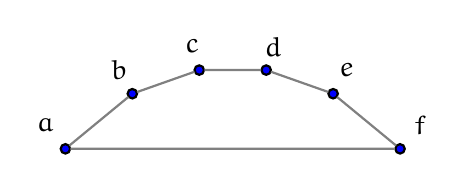
\begin{tikzpicture}[xscale=0.85]
\node at (-0.3,0.3) {$a$};
\node at (0.8,1) {$b$};
\node at (1.9,1.3) {$c$};
\node at (3.1,1.3) {$d$};
\node at (4.2,1) {$e$};
\node at (5.3,0.3) {$f$};
\node[draw,circle, thick, fill=blue, scale=0.3] (a) at (0,0) {};
\node[draw,circle, thick, fill=blue, scale=0.3] (b) at (1,0.7) {};
\node[draw,circle, thick, fill=blue, scale=0.3] (c) at (2,1) {};
\node[draw,circle, thick, fill=blue, scale=0.3] (d) at (3,1) {};
\node[draw,circle, thick, fill=blue, scale=0.3] (e) at (4,0.7) {};
\node[draw,circle, thick, fill=blue, scale=0.3] (f) at (5,0) {};
\draw[gray, thick] (a) -- (b) -- (c) -- (d) -- (e) -- (f) -- (a);
%\draw[gray] (a) -- (b) -- (c) -- (a);
%\draw[gray] (a) -- (c) -- (d) -- (a);
%\draw[gray] (a) -- (d) -- (e) -- (a);
%\draw[gray] (a) -- (e) -- (f) -- (a);
\end{tikzpicture}
\end{minipage}

\begin{minipage}{.47\textwidth}
\centering
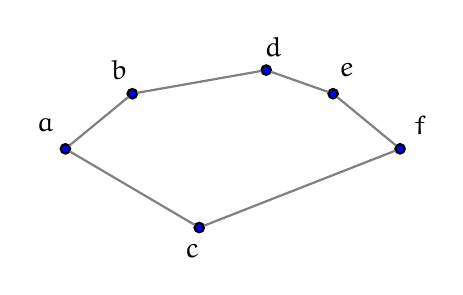
\begin{tikzpicture}[xscale=0.85]
\node at (-0.3,0.3) {$a$};
\node at (0.8,1) {$b$};
\node at (1.9,-1.3) {$c$};
\node at (3.1,1.3) {$d$};
\node at (4.2,1) {$e$};
\node at (5.3,0.3) {$f$};
\node[draw,circle, thick, fill=blue, scale=0.3] (a) at (0,0) {};
\node[draw,circle, thick, fill=blue, scale=0.3] (b) at (1,0.7) {};
\node[draw,circle, thick, fill=blue, scale=0.3] (c) at (2,-1) {};
\node[draw,circle, thick, fill=blue, scale=0.3] (d) at (3,1) {};
\node[draw,circle, thick, fill=blue, scale=0.3] (e) at (4,0.7) {};
\node[draw,circle, thick, fill=blue, scale=0.3] (f) at (5,0) {};
\draw[gray, thick] (a) -- (b) -- (d) -- (e) -- (f) -- (c) -- (a);
%\draw[gray] (a) -- (b) -- (d) -- (a);
%\draw[gray] (a) -- (c) -- (f) -- (a);
%\draw[gray] (a) -- (d) -- (e) -- (a);
%\draw[gray] (a) -- (e) -- (f) -- (a);
\end{tikzpicture}
\end{minipage}
\hfill
\begin{minipage}{.47\textwidth}
$O_{a,b,d} \lor O_{b,d,e} \lor O_{d,e,f} \lor \overline{O_{a,c,f}}$
\end{minipage}


\vspace{-10pt}

\begin{minipage}{.47\textwidth}
$O_{a,b,d} \lor O_{b,d,f} \lor \overline{O_{a,c,e}} \lor \overline{O_{c,e,f}}$
\end{minipage}
\hfill
\begin{minipage}{.47\textwidth}
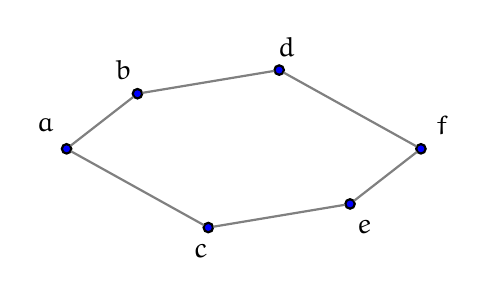
\begin{tikzpicture}[xscale=0.9]
\node at (-0.3,0.3) {$a$};
\node at (0.8,1) {$b$};
\node at (1.9,-1.3) {$c$};
\node at (3.1,1.3) {$d$};
\node at (4.2,-1) {$e$};
\node at (5.3,0.3) {$f$};
\node[draw,circle, thick, fill=blue, scale=0.3] (a) at (0,0) {};
\node[draw,circle, thick, fill=blue, scale=0.3] (b) at (1,0.7) {};
\node[draw,circle, thick, fill=blue, scale=0.3] (c) at (2,-1) {};
\node[draw,circle, thick, fill=blue, scale=0.3] (d) at (3,1) {};
\node[draw,circle, thick, fill=blue, scale=0.3] (e) at (4,-0.7) {};
\node[draw,circle, thick, fill=blue, scale=0.3] (f) at (5,0) {};
\draw[gray, thick] (a) -- (b) -- (d) -- (f) -- (e) -- (c) -- (a);
%\draw[gray] (a) -- (b) -- (d) -- (a);
%\draw[gray] (a) -- (c) -- (e) -- (a);
%\draw[gray] (a) -- (e) -- (f) -- (a);
%\draw[gray] (a) -- (d) -- (f) -- (a);
\end{tikzpicture}
\end{minipage}
}


\frame{
	\frametitle{Optimized $k$-Gon Encoding}

\large

\begin{minipage}{.47\textwidth}
%\centering
$x_{c,d} \lor O_{a,b,c} \lor O_{b,c,d}$\\
$\overline {x_{c,d}} \lor O_{c,d,e} \lor O_{d,e,f}$
\end{minipage}
\hfill
\begin{minipage}{.47\textwidth}
\centering
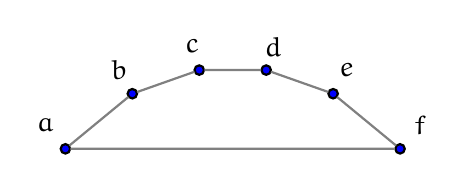
\begin{tikzpicture}[xscale=0.85]
\node at (-0.3,0.3) {$a$};
\node at (0.8,1) {$b$};
\node at (1.9,1.3) {$c$};
\node at (3.1,1.3) {$d$};
\node at (4.2,1) {$e$};
\node at (5.3,0.3) {$f$};
\node[draw,circle, thick, fill=blue, scale=0.3] (a) at (0,0) {};
\node[draw,circle, thick, fill=blue, scale=0.3] (b) at (1,0.7) {};
\node[draw,circle, thick, fill=blue, scale=0.3] (c) at (2,1) {};
\node[draw,circle, thick, fill=blue, scale=0.3] (d) at (3,1) {};
\node[draw,circle, thick, fill=blue, scale=0.3] (e) at (4,0.7) {};
\node[draw,circle, thick, fill=blue, scale=0.3] (f) at (5,0) {};
\draw[gray, thick] (a) -- (b) -- (c) -- (d) -- (e) -- (f) -- (a);
%\draw[gray] (a) -- (b) -- (c) -- (a);
%\draw[gray] (a) -- (c) -- (d) -- (a);
%\draw[gray] (a) -- (d) -- (e) -- (a);
%\draw[gray] (a) -- (e) -- (f) -- (a);
\end{tikzpicture}
\end{minipage}

\begin{minipage}{.47\textwidth}
\centering
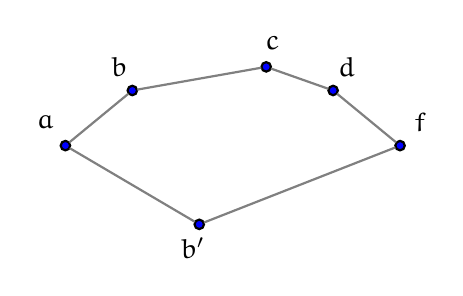
\begin{tikzpicture}[xscale=0.85]
\node at (-0.3,0.3) {$a$};
\node at (0.8,1) {$b$};
\node at (1.9,-1.3) {$b^{\prime}$};
\node at (3.1,1.3) {$c$};
\node at (4.2,1) {$d$};
\node at (5.3,0.3) {$f$};
\node[draw,circle, thick, fill=blue, scale=0.3] (a) at (0,0) {};
\node[draw,circle, thick, fill=blue, scale=0.3] (b) at (1,0.7) {};
\node[draw,circle, thick, fill=blue, scale=0.3] (c) at (2,-1) {};
\node[draw,circle, thick, fill=blue, scale=0.3] (d) at (3,1) {};
\node[draw,circle, thick, fill=blue, scale=0.3] (e) at (4,0.7) {};
\node[draw,circle, thick, fill=blue, scale=0.3] (f) at (5,0) {};
\draw[gray, thick] (a) -- (b) -- (d) -- (e) -- (f) -- (c) -- (a);
%\draw[gray] (a) -- (b) -- (d) -- (a);
%\draw[gray] (a) -- (c) -- (f) -- (a);
%\draw[gray] (a) -- (d) -- (e) -- (a);
%\draw[gray] (a) -- (e) -- (f) -- (a);
\end{tikzpicture}
\end{minipage}
\hfill
\begin{minipage}{.47\textwidth}
%\centering
$y_{a,f} \lor O_{a,b,c} \lor O_{b,c,d} \lor O_{c,d,f}$
$\overline{y_{a,f}} \lor \overline{O_{a,b^{\prime},f}}$

\end{minipage}


\vspace{-10pt}

\begin{minipage}{.47\textwidth}
%\centering
$z_{a,f} \lor O_{a,b,c} \lor O_{b,c,f}$\\
$\overline{z_{a,f}} \lor \overline{O_{a,b^{\prime},c^{\prime}}} \lor \overline{O_{b^{\prime},c^{\prime},f}}$\end{minipage}
\hfill
\begin{minipage}{.47\textwidth}
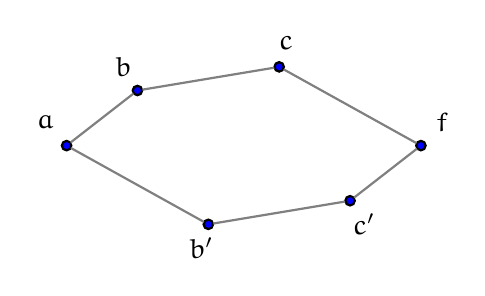
\begin{tikzpicture}[xscale=0.9]
\node at (-0.3,0.3) {$a$};
\node at (0.8,1) {$b$};
\node at (1.9,-1.3) {$b^{\prime}$};
\node at (3.1,1.3) {$c$};
\node at (4.2,-1) {$c^{\prime}$};
\node at (5.3,0.3) {$f$};
\node[draw,circle, thick, fill=blue, scale=0.3] (a) at (0,0) {};
\node[draw,circle, thick, fill=blue, scale=0.3] (b) at (1,0.7) {};
\node[draw,circle, thick, fill=blue, scale=0.3] (c) at (2,-1) {};
\node[draw,circle, thick, fill=blue, scale=0.3] (d) at (3,1) {};
\node[draw,circle, thick, fill=blue, scale=0.3] (e) at (4,-0.7) {};
\node[draw,circle, thick, fill=blue, scale=0.3] (f) at (5,0) {};
\draw[gray, thick] (a) -- (b) -- (d) -- (f) -- (e) -- (c) -- (a);
%\draw[gray] (a) -- (b) -- (d) -- (a);
%\draw[gray] (a) -- (c) -- (e) -- (a);
%\draw[gray] (a) -- (e) -- (f) -- (a);
%\draw[gray] (a) -- (d) -- (f) -- (a);
\end{tikzpicture}
\end{minipage}
}
\fi

\frame{
	\frametitle{Inside Variables}

\large

We introduce \structure{inside variables} $I_{x;a,b,c}$ which are true
if and only if point $x$ is in the triangle $abc$ with $a < x < b$
or $b < x < c$.

\bigskip

\begin{minipage}{.6\textwidth}
${I_{x;a,b,c}} \lor \overline{O_{a,b,c}} \lor {O_{a,x,b}} \lor \overline{O_{x,b,c}} \lor \overline{O_{a,x,c}}$\\[3pt]
$\overline{I_{x;a,b,c}} \lor \overline{O_{a,b,c}} \lor \overline{O_{a,x,b}}$\\[3pt]
$\overline{I_{x;a,b,c}} \lor \overline{O_{a,b,c}} \lor O_{x,b,c}$\\[3pt]
$\overline{I_{x;a,b,c}} \lor \overline{O_{a,b,c}} \lor O_{a,x,c}$\\[3pt]
\end{minipage}
%\hfill
\begin{minipage}{.35\textwidth}
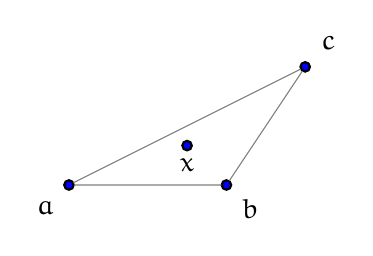
\begin{tikzpicture}

\node at (-0.3,-0.3) {$a$};
\node at (2.3,-0.3) {$b$};
\node at (3.3,1.8) {$c$};
\node at (1.5,0.25) {$x$};
\node[draw,circle, thick, fill=blue, scale=0.3] (a) at (0,0) {};
\node[draw,circle, thick, fill=blue, scale=0.3] (b) at (2,0) {};
\node[draw,circle, thick, fill=blue, scale=0.3] (c) at (3,1.5) {};
\node[draw,circle, thick, fill=blue, scale=0.3] (x) at (1.5,0.5) {};
\draw[gray] (a) -- (b) -- (c) -- (a);
\end{tikzpicture}
\end{minipage}

\pause
\bigskip

\begin{minipage}{.6\textwidth}

${I_{x;a,b,c}} \lor {O_{a,b,c}} \lor \overline{O_{a,x,b}} \lor O_{x,b,c} \lor O_{a,x,c}$\\[3pt]
$\overline{I_{x;a,b,c}} \lor {O_{a,b,c}} \lor {O_{a,x,b}}$\\[3pt]
$\overline{I_{x;a,b,c}} \lor {O_{a,b,c}} \lor \overline{O_{x,b,c}}$\\[3pt]
$\overline{I_{x;a,b,c}} \lor {O_{a,b,c}} \lor \overline{O_{a,x,c}}$\\[3pt]
\end{minipage}
\begin{minipage}{.35\textwidth}
\bigskip
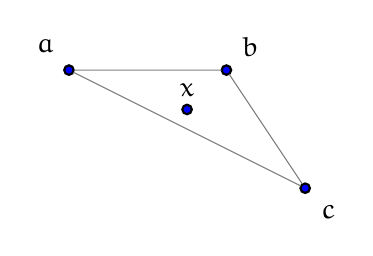
\begin{tikzpicture}

\node at (-0.3,0.3) {$a$};
\node at (2.3,0.3) {$b$};
\node at (3.3,-1.8) {$c$};
\node at (1.5,-0.25) {$x$};
\node[draw,circle, thick, fill=blue, scale=0.3] (a) at (0,0) {};
\node[draw,circle, thick, fill=blue, scale=0.3] (b) at (2,0) {};
\node[draw,circle, thick, fill=blue, scale=0.3] (c) at (3,-1.5) {};
\node[draw,circle, thick, fill=blue, scale=0.3] (x) at (1.5,-0.5) {};
\draw[gray] (a) -- (b) -- (c) -- (a);
\end{tikzpicture}
\end{minipage}

%  printf ("%i %i %i 0\n", -d,  t, -abx);
%  printf ("%i %i %i 0\n", -d,  t, -bcx);
%  printf ("%i %i %i 0\n", -d,  t, -acx);
%
%  printf ("%i %i %i 0\n", -d, -t,  abx);
%  printf ("%i %i %i 0\n", -d, -t,  bcx);
%  printf ("%i %i %i 0\n", -d, -t,  acx);
%
%#ifdef BLOCKED
%  printf ("%i %i %i %i %i 0\n", d,  t,  abx,  bcx,  acx);
%  printf ("%i %i %i %i %i 0\n", d, -t, -abx, -bcx, -acx);
%#endif

}

\frame{
	\frametitle{Hole Variables}
	
\large

We introduce \structure{hole variables} $H_{a,b,c}$ which are true
if and only if no points occur with the triangle $abc$ with $a < b < c$.

\medskip

\[
H_{a,b,c} \lor \bigvee_{a < x < c} {I_{x;a,b,c}}
\]

\[
\bigwedge_{a < x < c} \overline{H_{a,b,c}} \lor \overline{I_{x;a,b,c}}~~~~~~~\mathrm{(redundant)}
\]

\bigskip
\pause

Simple $6$-hole encoding:

\begin{center}
$(\bigvee_{a,b,c \in X} \overline{H_{a,b,c}})$~~~~$\forall~X \subset S$ with $|X| = 6$
\end{center}

}

\iffalse
\frame{
	\frametitle{$k$-Hole Encoding}

\large

\bigskip

\begin{minipage}{.52\textwidth}
%\centering
$O_{a,b,c} \lor O_{b,c,d} \lor O_{c,d,e} \lor O_{d,e,f}~\lor$\\[3pt]
$\overline{H_{a,b,c}} \lor \overline{H_{a,c,d}} \lor \overline{H_{a,d,e}} \lor \overline{H_{a,e,f}}$\\
\end{minipage}
\hfill
\begin{minipage}{.45\textwidth}
\centering
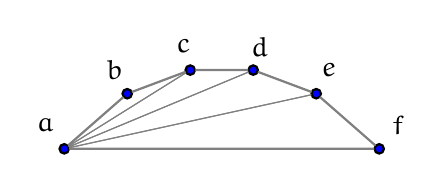
\begin{tikzpicture}[xscale=0.8]
\node at (-0.3,0.3) {$a$};
\node at (0.8,1) {$b$};
\node at (1.9,1.3) {$c$};
\node at (3.1,1.3) {$d$};
\node at (4.2,1) {$e$};
\node at (5.3,0.3) {$f$};
\node[draw,circle, thick, fill=blue, scale=0.3] (a) at (0,0) {};
\node[draw,circle, thick, fill=blue, scale=0.3] (b) at (1,0.7) {};
\node[draw,circle, thick, fill=blue, scale=0.3] (c) at (2,1) {};
\node[draw,circle, thick, fill=blue, scale=0.3] (d) at (3,1) {};
\node[draw,circle, thick, fill=blue, scale=0.3] (e) at (4,0.7) {};
\node[draw,circle, thick, fill=blue, scale=0.3] (f) at (5,0) {};
\draw[gray, thick] (a) -- (b) -- (c) -- (d) -- (e) -- (f) -- (a);
\draw[gray] (a) -- (b) -- (c) -- (a);
\draw[gray] (a) -- (c) -- (d) -- (a);
\draw[gray] (a) -- (d) -- (e) -- (a);
\draw[gray] (a) -- (e) -- (f) -- (a);
\end{tikzpicture}
\end{minipage}

\begin{minipage}{.45\textwidth}
\centering
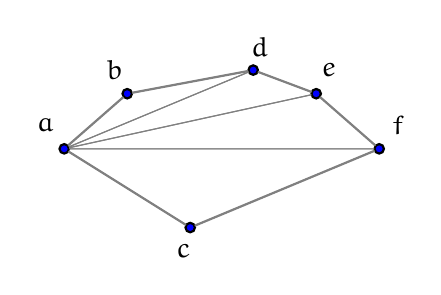
\begin{tikzpicture}[xscale=0.8]
\node at (-0.3,0.3) {$a$};
\node at (0.8,1) {$b$};
\node at (1.9,-1.3) {$c$};
\node at (3.1,1.3) {$d$};
\node at (4.2,1) {$e$};
\node at (5.3,0.3) {$f$};
\node[draw,circle, thick, fill=blue, scale=0.3] (a) at (0,0) {};
\node[draw,circle, thick, fill=blue, scale=0.3] (b) at (1,0.7) {};
\node[draw,circle, thick, fill=blue, scale=0.3] (c) at (2,-1) {};
\node[draw,circle, thick, fill=blue, scale=0.3] (d) at (3,1) {};
\node[draw,circle, thick, fill=blue, scale=0.3] (e) at (4,0.7) {};
\node[draw,circle, thick, fill=blue, scale=0.3] (f) at (5,0) {};
\draw[gray, thick] (a) -- (b) -- (d) -- (e) -- (f) -- (c) -- (a);
\draw[gray] (a) -- (b) -- (d) -- (a);
\draw[gray] (a) -- (c) -- (f) -- (a);
\draw[gray] (a) -- (d) -- (e) -- (a);
\draw[gray] (a) -- (e) -- (f) -- (a);
\end{tikzpicture}
\end{minipage}
\hfill
\begin{minipage}{.52\textwidth}
$O_{a,b,d} \lor O_{b,d,e} \lor O_{d,e,f} \lor \overline{O_{a,c,f}}~\lor$\\[3pt]
$\overline{H_{a,b,d}} \lor \overline{H_{a,d,e}} \lor \overline{H_{a,e,f}} \lor \overline{H_{a,c,f}}$
\end{minipage}


\vspace{-10pt}

\begin{minipage}{.52\textwidth}
$O_{a,b,d} \lor O_{b,d,f} \lor \overline{O_{a,c,e}} \lor \overline{O_{c,e,f}}~\lor$
$\overline{H_{a,b,d}} \lor \overline{H_{a,d,f}} \lor \overline{H_{a,c,e}} \lor \overline{H_{a,e,f}}$

\end{minipage}
\hfill
\begin{minipage}{.45\textwidth}
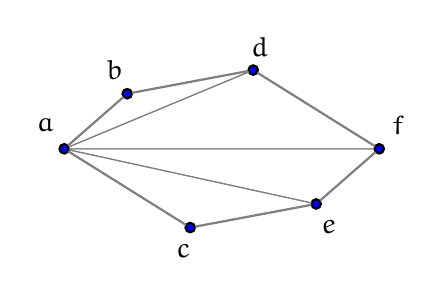
\begin{tikzpicture}[xscale=0.8]
\node at (-0.3,0.3) {$a$};
\node at (0.8,1) {$b$};
\node at (1.9,-1.3) {$c$};
\node at (3.1,1.3) {$d$};
\node at (4.2,-1) {$e$};
\node at (5.3,0.3) {$f$};
\node[draw,circle, thick, fill=blue, scale=0.3] (a) at (0,0) {};
\node[draw,circle, thick, fill=blue, scale=0.3] (b) at (1,0.7) {};
\node[draw,circle, thick, fill=blue, scale=0.3] (c) at (2,-1) {};
\node[draw,circle, thick, fill=blue, scale=0.3] (d) at (3,1) {};
\node[draw,circle, thick, fill=blue, scale=0.3] (e) at (4,-0.7) {};
\node[draw,circle, thick, fill=blue, scale=0.3] (f) at (5,0) {};
\draw[gray, thick] (a) -- (b) -- (d) -- (f) -- (e) -- (c) -- (a);
\draw[gray] (a) -- (b) -- (d) -- (a);
\draw[gray] (a) -- (c) -- (e) -- (a);
\draw[gray] (a) -- (e) -- (f) -- (a);
\draw[gray] (a) -- (d) -- (f) -- (a);
\end{tikzpicture}
\end{minipage}
}
\fi

\frame{
	\frametitle{$k$-Hole Encoding (I)}

\large

Simple $6$-hole encoding with $O(n^6)$ clauses with \structure{20 literals}:
\begin{center}
$(\bigvee_{a,b,c \in X} \overline{H_{a,b,c}})$~~~~$\forall~X \subset S$ with $|X| = 6$
\end{center}

\medskip
\pause

Shorter clauses, thus \structure{more propagation}, but still $O(n^6)$

\begin{minipage}{.52\textwidth}
$O_{a,b,d} \lor O_{b,d,f} \lor \overline{O_{a,c,e}} \lor \overline{O_{c,e,f}}~\lor$
$\overline{H_{a,b,d}} \lor \overline{H_{a,d,f}} \lor \overline{H_{a,c,e}} \lor \overline{H_{a,e,f}}$
\end{minipage}
\hfill
\begin{minipage}{.45\textwidth}
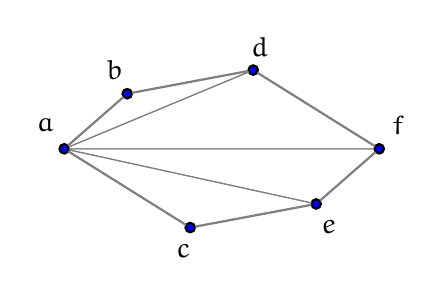
\begin{tikzpicture}[xscale=0.8]
\node at (-0.3,0.3) {$a$};
\node at (0.8,1) {$b$};
\node at (1.9,-1.3) {$c$};
\node at (3.1,1.3) {$d$};
\node at (4.2,-1) {$e$};
\node at (5.3,0.3) {$f$};
\node[draw,circle, thick, fill=blue, scale=0.3] (a) at (0,0) {};
\node[draw,circle, thick, fill=blue, scale=0.3] (b) at (1,0.7) {};
\node[draw,circle, thick, fill=blue, scale=0.3] (c) at (2,-1) {};
\node[draw,circle, thick, fill=blue, scale=0.3] (d) at (3,1) {};
\node[draw,circle, thick, fill=blue, scale=0.3] (e) at (4,-0.7) {};
\node[draw,circle, thick, fill=blue, scale=0.3] (f) at (5,0) {};
\draw[gray, thick] (a) -- (b) -- (d) -- (f) -- (e) -- (c) -- (a);
\draw[gray] (a) -- (b) -- (d) -- (a);
\draw[gray] (a) -- (c) -- (e) -- (a);
\draw[gray] (a) -- (e) -- (f) -- (a);
\draw[gray] (a) -- (d) -- (f) -- (a);
\end{tikzpicture}
\end{minipage}

\medskip
\pause

\structure{Auxiliary variables} make an $O(n^4)$ clauses encoding possible
\begin{eqnarray*}
&\!\!\!\!\!\!\!\!\!\!\!\!\!\! x_{a,f} \lor O_{a,b,d} \lor O_{b,d,f} \lor \overline{H_{a,b,d}} \lor \overline{H_{a,d,f}}&\mathrm{with~}a < b < d < f\\
&\!\!\!\!\!\!\!\!\!\!\!\!\!\! \overline{x_{a,f}} \lor \overline{O_{a,c,e}} \lor \overline{O_{c,e,f}} \lor \overline{H_{a,c,e}} \lor \overline{H_{a,e,f}}&\mathrm{with~}a < c < e < f
\end{eqnarray*}

}


\frame{
	\frametitle{$k$-Hole Encoding (II)}

\large

Shorter clauses, thus \structure{more propagation}, but still $O(n^6)$

\bigskip

\begin{minipage}{.52\textwidth}
%\centering
\medskip
$O_{a,b,c} \lor O_{b,c,d} \lor O_{c,d,e} \lor O_{d,e,f}~\lor$\\[3pt]
$\overline{H_{a,b,c}} \lor \overline{H_{a,c,d}} \lor \overline{H_{a,d,e}} \lor \overline{H_{a,e,f}}$\\
\end{minipage}
\hfill
\begin{minipage}{.45\textwidth}
\centering
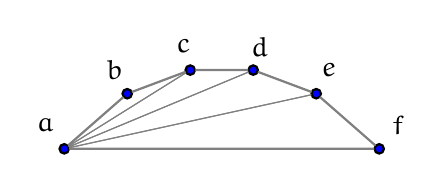
\begin{tikzpicture}[xscale=0.8]
\node at (-0.3,0.3) {$a$};
\node at (0.8,1) {$b$};
\node at (1.9,1.3) {$c$};
\node at (3.1,1.3) {$d$};
\node at (4.2,1) {$e$};
\node at (5.3,0.3) {$f$};
\node[draw,circle, thick, fill=blue, scale=0.3] (a) at (0,0) {};
\node[draw,circle, thick, fill=blue, scale=0.3] (b) at (1,0.7) {};
\node[draw,circle, thick, fill=blue, scale=0.3] (c) at (2,1) {};
\node[draw,circle, thick, fill=blue, scale=0.3] (d) at (3,1) {};
\node[draw,circle, thick, fill=blue, scale=0.3] (e) at (4,0.7) {};
\node[draw,circle, thick, fill=blue, scale=0.3] (f) at (5,0) {};
\draw[gray, thick] (a) -- (b) -- (c) -- (d) -- (e) -- (f) -- (a);
\draw[gray] (a) -- (b) -- (c) -- (a);
\draw[gray] (a) -- (c) -- (d) -- (a);
\draw[gray] (a) -- (d) -- (e) -- (a);
\draw[gray] (a) -- (e) -- (f) -- (a);
\end{tikzpicture}
\end{minipage}

\bigskip
\bigskip
\pause

\structure{Auxiliary variables} make an $O(n^4)$ clauses encoding possible
\begin{eqnarray*}
&\!\!\!\!\!\!\!\!\!\!\!\!\!\! y_{a,c,d} \lor O_{a,b,c} \lor O_{b,c,d} \lor \overline{H_{a,b,c}} \lor \overline{H_{a,c,d}}&\mathrm{with~}a < b < c < d\\
&\!\!\!\!\! z_{a,d,e} \lor \overline{O_{c,d,e}} \lor \overline{H_{a,d,e}} \lor \overline{y_{a,c,d}}&\mathrm{with~}a < c < d < e\\
&\!\!\!\!\!  \overline{O_{d,e,f}} \lor \overline{H_{a,e,f}} \lor \overline{z_{a,d,e}}&\mathrm{with~}a < d < e < f
\end{eqnarray*}




}

\section{Results}
\frame{\Large \tableofcontents[currentsection]}

\frame{
	\frametitle{Comparison to Existing Work}

\large

Szekeres and Peters (2006) solved $g(6) =17$ in 63 CPU days\!\!\!\!\!
\begin{itemize}
\item Roughly 40 CPU hours on today's hardware
\item \url{https://www.cpubenchmark.net/year-on-year.html}
\end{itemize}

\bigskip

SAT solving, using the same abstraction, is much faster
\begin{itemize}
\item The independent SAT-approaches by Marić and Scheucher required a few CPU hours
\item Their encodings consist of $O(n^k)$ clauses
\end{itemize}

\bigskip

Our $O(n^4)$ encoding for $k$-gons and $k$-holes is even faster
\begin{itemize}
\item $g(6) =17$ can be solved in 20 CPU seconds
\item Roughly 4 orders of magnitude faster than to original proof
\end{itemize} 


}


\frame{
	\frametitle{Problem Partitioning}

\large

%The interesting problems are too hard for a single CPU
%
%\bigskip

We developed a partitioning algorithm to split the problem
into thousands much easier subproblems
\begin{itemize}
\item Original problem UNSAT iff all subproblems UNSAT
\item Two parameters: start ($a$) and length ($\ell$)
\item Tested on: 24 points contain $6$-hole \structure{or} $7$-gon
\end{itemize}

\medskip

\begin{tabular}{@{~~~}c@{~~~}r@{~~~}r@{~~~}r@{~~~}r@{~~~}r@{~~~}r@{~~~}c}
\toprule
$a$ & $\ell$~ & $\#$cubes & avg time (s) & max time (s) & total (h)\\
\midrule
2 & 21 & 312\,418 & 20.43~~  & 218.37~~~ & 1\,773.38~\\
3 & 19 & 89\,384 & 43.25~~ & 410.09~~~ & 1\,073.91~\\
4 & 17 & 25\,663 & 113.12~~ & 1\,080.84~~~ & 806.37~\\
5 & 15 & 7393 & 355.46~~ & 2\,884.46~~~ & 729.98~\\
6 & 13 & 2149 & 1\,223.58~~ & 8\,776.65~~~ & 730.41~\\
7 & 11 & 629 & 4\,647.19~~ & 24\,232.12~~~ & 811.97~\\
8 & 9 & 188 & 17\,414.70~~ & 55\,799.72~~~ & 909.44~\\
\bottomrule
\end{tabular}
	
}


\frame{
	\frametitle{Runtime distribution on $6$-hole or $7$-gon}


\parindent -15pt


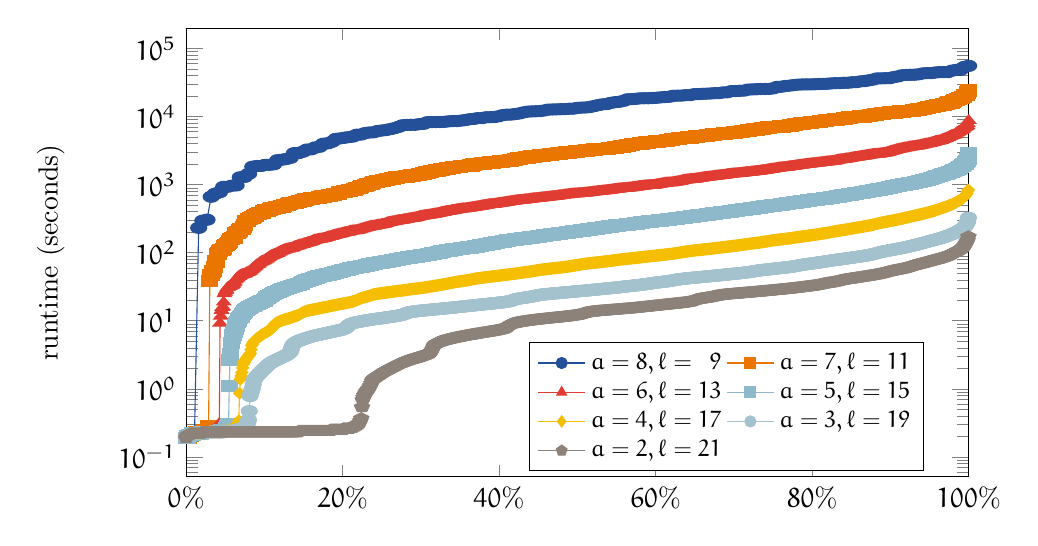
\begin{tikzpicture}
          \begin{axis}[xmin=0,xmax=1, scaled x ticks = false, xticklabel={$\pgfmathprintnumber{\fpeval{\tick*100}}\%$}, legend style={nodes={scale=0.85]}, legend columns=2, at={(0.65,0.3)}}, ymode=log, yscale=1, xscale=1.45,ylabel={runtime (seconds)}]

\addplot[color=colg, mark=*] coordinates
{(0.00531915,0.22) (0.0106383,0.22) (0.0159574,232.07) (0.0212766,295.47) (0.0265957,305.82) (0.0319149,664.77) (0.037234,738.34) (0.0425532,772.81) (0.0478723,928.52) (0.0531915,932.07) (0.0585106,967.97) (0.0638298,974.95) (0.0691489,1286.00) (0.0744681,1299.92) (0.0797872,1443.38) (0.0851064,1839.01) (0.0904255,1881.59) (0.0957447,1886.24) (0.101064,1956.33) (0.106383,1959.06) (0.111702,1991.17) (0.117021,2293.80) (0.12234,2327.86) (0.12766,2383.75) (0.132979,2475.15) (0.138298,2911.25) (0.143617,2916.18) (0.148936,3044.51) (0.154255,3285.26) (0.159574,3301.99) (0.164894,3530.44) (0.170213,3601.25) (0.175532,4004.91) (0.180851,4050.64) (0.18617,4265.23) (0.191489,4711.89) (0.196809,4794.54) (0.202128,4891.17) (0.207447,5002.26) (0.212766,5090.84) (0.218085,5431.50) (0.223404,5451.43) (0.228723,5735.27) (0.234043,5846.70) (0.239362,5887.15) (0.244681,6146.78) (0.25,6257.85) (0.255319,6362.07) (0.260638,6549.89) (0.265957,6757.20) (0.271277,7061.79) (0.276596,7474.53) (0.281915,7558.32) (0.287234,7592.55) (0.292553,7596.07) (0.297872,7761.10) (0.303191,7839.59) (0.308511,8295.99) (0.31383,8314.48) (0.319149,8332.96) (0.324468,8349.74) (0.329787,8390.06) (0.335106,8530.08) (0.340426,8607.02) (0.345745,8617.39) (0.351064,8736.56) (0.356383,8903.50) (0.361702,9146.60) (0.367021,9254.15) (0.37234,9499.05) (0.37766,9507.07) (0.382979,9787.01) (0.388298,9825.75) (0.393617,9863.74) (0.398936,10104.12) (0.404255,10510.38) (0.409574,10701.69) (0.414894,10707.01) (0.420213,10920.94) (0.425532,11128.79) (0.430851,11538.71) (0.43617,11856.29) (0.441489,11939.83) (0.446809,12006.04) (0.452128,12086.45) (0.457447,12323.02) (0.462766,12688.86) (0.468085,12751.45) (0.473404,12803.46) (0.478723,12868.38) (0.484043,12905.23) (0.489362,13071.97) (0.494681,13088.42) (0.5,13443.70) (0.505319,13590.61) (0.510638,13651.72) (0.515957,13857.49) (0.521277,14293.32) (0.526596,14777.89) (0.531915,15174.62) (0.537234,15311.18) (0.542553,15916.92) (0.547872,16301.70) (0.553191,16519.96) (0.558511,17022.55) (0.56383,17985.20) (0.569149,18085.71) (0.574468,18274.59) (0.579787,18592.21) (0.585106,18643.55) (0.590426,18651.12) (0.595745,18766.66) (0.601064,18946.88) (0.606383,19208.02) (0.611702,19434.06) (0.617021,19566.75) (0.62234,20250.45) (0.62766,20358.02) (0.632979,20383.03) (0.638298,20688.48) (0.643617,20709.15) (0.648936,21357.81) (0.654255,21478.37) (0.659574,21655.37) (0.664894,21756.87) (0.670213,21914.97) (0.675532,22129.40) (0.680851,22180.71) (0.68617,22698.04) (0.691489,22823.90) (0.696809,23704.52) (0.702128,23788.02) (0.707447,23992.83) (0.712766,24153.91) (0.718085,24994.78) (0.723404,25154.08) (0.728723,25286.86) (0.734043,25517.25) (0.739362,25529.05) (0.744681,25556.28) (0.75,26016.65) (0.755319,27368.04) (0.760638,27545.70) (0.765957,28215.95) (0.771277,28586.38) (0.776596,29136.45) (0.781915,29574.49) (0.787234,29743.16) (0.792553,29814.28) (0.797872,29815.62) (0.803191,29940.04) (0.808511,30167.26) (0.81383,30310.65) (0.819149,30429.40) (0.824468,30854.54) (0.829787,31055.18) (0.835106,31059.44) (0.840426,31468.94) (0.845745,31503.65) (0.851064,32044.89) (0.856383,32153.14) (0.861702,33022.63) (0.867021,33344.70) (0.87234,34192.27) (0.87766,35076.50) (0.882979,36457.28) (0.888298,36558.12) (0.893617,36731.29) (0.898936,36769.72) (0.904255,38127.78) (0.909574,38997.07) (0.914894,40583.76) (0.920213,40990.87) (0.925532,41260.47) (0.930851,41314.45) (0.93617,41959.91) (0.941489,43244.90) (0.946809,43637.96) (0.952128,43674.04) (0.957447,44574.71) (0.962766,45154.43) (0.968085,45176.42) (0.973404,45227.60) (0.978723,47532.73) (0.984043,48592.43) (0.989362,48728.10) (0.994681,53846.60) (1,55799.72)};

\addplot[color=colf, mark=square*] coordinates
          {(0.00158983,0.19) (0.00317965,0.19) (0.00476948,0.20) (0.0063593,0.21) (0.00794913,0.21) (0.00953895,0.22) (0.0111288,0.22) (0.0127186,0.23) (0.0143084,0.23) (0.0158983,0.23) (0.0174881,0.23) (0.0190779,0.23) (0.0206677,0.23) (0.0222576,0.24) (0.0238474,0.25) (0.0254372,0.25) (0.027027,0.25) (0.0286169,0.28) (0.0302067,38.52) (0.0317965,46.98) (0.0333863,53.11) (0.0349762,54.52) (0.036566,61.61) (0.0381558,74.50) (0.0397456,96.94) (0.0413355,97.43) (0.0429253,106.48) (0.0445151,108.23) (0.0461049,109.36) (0.0476948,113.24) (0.0492846,125.98) (0.0508744,128.47) (0.0524642,135.69) (0.0540541,140.69) (0.0556439,145.87) (0.0572337,157.02) (0.0588235,164.45) (0.0604134,165.53) (0.0620032,167.31) (0.063593,193.23) (0.0651828,198.25) (0.0667727,203.83) (0.0683625,212.57) (0.0699523,223.79) (0.0715421,224.69) (0.073132,236.14) (0.0747218,252.76) (0.0763116,291.85) (0.0779014,293.55) (0.0794913,310.69) (0.0810811,314.94) (0.0826709,325.19) (0.0842607,328.77) (0.0858506,334.34) (0.0874404,346.44) (0.0890302,351.40) (0.09062,370.41) (0.0922099,372.34) (0.0937997,378.75) (0.0953895,380.80) (0.0969793,385.50) (0.0985692,406.35) (0.100159,406.39) (0.101749,416.28) (0.103339,417.25) (0.104928,419.55) (0.106518,424.41) (0.108108,433.64) (0.109698,445.39) (0.111288,452.36) (0.112878,455.77) (0.114467,457.00) (0.116057,461.26) (0.117647,470.33) (0.119237,472.78) (0.120827,476.19) (0.122417,478.72) (0.124006,488.93) (0.125596,497.42) (0.127186,505.70) (0.128776,508.99) (0.130366,516.91) (0.131955,529.22) (0.133545,531.30) (0.135135,532.38) (0.136725,534.85) (0.138315,538.64) (0.139905,540.10) (0.141494,556.58) (0.143084,564.16) (0.144674,571.49) (0.146264,573.15) (0.147854,574.34) (0.149444,586.18) (0.151033,593.35) (0.152623,607.11) (0.154213,608.24) (0.155803,609.24) (0.157393,617.96) (0.158983,620.16) (0.160572,624.92) (0.162162,635.30) (0.163752,641.49) (0.165342,643.98) (0.166932,644.36) (0.168521,645.31) (0.170111,658.50) (0.171701,662.49) (0.173291,665.39) (0.174881,669.49) (0.176471,677.37) (0.17806,681.58) (0.17965,682.22) (0.18124,691.08) (0.18283,694.41) (0.18442,695.73) (0.18601,701.38) (0.187599,703.64) (0.189189,720.32) (0.190779,722.38) (0.192369,726.66) (0.193959,733.03) (0.195548,779.97) (0.197138,786.64) (0.198728,787.85) (0.200318,791.55) (0.201908,794.66) (0.203498,809.53) (0.205087,815.56) (0.206677,817.16) (0.208267,822.18) (0.209857,827.47) (0.211447,832.60) (0.213037,847.09) (0.214626,851.65) (0.216216,853.98) (0.217806,881.96) (0.219396,886.01) (0.220986,888.06) (0.222576,915.81) (0.224165,948.51) (0.225755,952.86) (0.227345,967.55) (0.228935,973.75) (0.230525,991.49) (0.232114,1007.63) (0.233704,1014.63) (0.235294,1020.51) (0.236884,1035.45) (0.238474,1068.48) (0.240064,1096.47) (0.241653,1100.40) (0.243243,1102.36) (0.244833,1122.97) (0.246423,1132.34) (0.248013,1140.44) (0.249603,1143.89) (0.251192,1145.17) (0.252782,1160.68) (0.254372,1161.10) (0.255962,1168.24) (0.257552,1214.15) (0.259141,1218.81) (0.260731,1226.24) (0.262321,1228.74) (0.263911,1233.69) (0.265501,1252.22) (0.267091,1256.42) (0.26868,1273.66) (0.27027,1281.07) (0.27186,1290.08) (0.27345,1294.38) (0.27504,1302.78) (0.27663,1303.40) (0.278219,1306.47) (0.279809,1308.53) (0.281399,1320.10) (0.282989,1338.21) (0.284579,1347.36) (0.286169,1351.86) (0.287758,1367.93) (0.289348,1367.95) (0.290938,1374.71) (0.292528,1375.35) (0.294118,1394.65) (0.295707,1395.66) (0.297297,1406.15) (0.298887,1420.26) (0.300477,1448.46) (0.302067,1449.08) (0.303657,1459.39) (0.305246,1480.16) (0.306836,1506.66) (0.308426,1509.58) (0.310016,1520.76) (0.311606,1553.07) (0.313196,1576.91) (0.314785,1582.37) (0.316375,1591.81) (0.317965,1609.41) (0.319555,1616.03) (0.321145,1618.64) (0.322734,1642.76) (0.324324,1655.98) (0.325914,1670.50) (0.327504,1680.88) (0.329094,1683.55) (0.330684,1697.88) (0.332273,1716.51) (0.333863,1725.90) (0.335453,1742.75) (0.337043,1761.75) (0.338633,1763.30) (0.340223,1778.98) (0.341812,1794.80) (0.343402,1813.08) (0.344992,1818.69) (0.346582,1823.85) (0.348172,1834.58) (0.349762,1840.59) (0.351351,1858.23) (0.352941,1860.15) (0.354531,1860.73) (0.356121,1884.12) (0.357711,1888.70) (0.3593,1898.09) (0.36089,1899.97) (0.36248,1906.36) (0.36407,1909.66) (0.36566,1927.54) (0.36725,1976.24) (0.368839,1988.99) (0.370429,2008.02) (0.372019,2010.84) (0.373609,2028.15) (0.375199,2029.19) (0.376789,2038.33) (0.378378,2043.53) (0.379968,2050.43) (0.381558,2056.66) (0.383148,2069.95) (0.384738,2075.97) (0.386328,2088.09) (0.387917,2103.21) (0.389507,2113.89) (0.391097,2117.82) (0.392687,2130.43) (0.394277,2137.33) (0.395866,2139.80) (0.397456,2141.78) (0.399046,2153.20) (0.400636,2166.60) (0.402226,2192.95) (0.403816,2202.45) (0.405405,2218.38) (0.406995,2222.46) (0.408585,2228.33) (0.410175,2236.95) (0.411765,2245.40) (0.413355,2256.79) (0.414944,2265.33) (0.416534,2310.48) (0.418124,2325.87) (0.419714,2334.06) (0.421304,2390.39) (0.422893,2411.30) (0.424483,2421.80) (0.426073,2422.12) (0.427663,2451.26) (0.429253,2473.31) (0.430843,2475.31) (0.432432,2488.89) (0.434022,2500.16) (0.435612,2503.93) (0.437202,2539.36) (0.438792,2570.03) (0.440382,2575.14) (0.441971,2592.51) (0.443561,2600.15) (0.445151,2609.77) (0.446741,2613.50) (0.448331,2641.83) (0.449921,2652.08) (0.45151,2667.79) (0.4531,2678.13) (0.45469,2685.48) (0.45628,2696.61) (0.45787,2711.01) (0.459459,2719.90) (0.461049,2721.61) (0.462639,2727.30) (0.464229,2742.51) (0.465819,2775.47) (0.467409,2817.25) (0.468998,2821.87) (0.470588,2822.13) (0.472178,2845.20) (0.473768,2850.43) (0.475358,2877.33) (0.476948,2881.26) (0.478537,2891.06) (0.480127,2906.82) (0.481717,2909.94) (0.483307,2924.19) (0.484897,2952.12) (0.486486,2980.93) (0.488076,2981.16) (0.489666,3017.75) (0.491256,3020.38) (0.492846,3028.91) (0.494436,3031.91) (0.496025,3039.60) (0.497615,3058.39) (0.499205,3067.26) (0.500795,3090.59) (0.502385,3099.10) (0.503975,3103.31) (0.505564,3116.59) (0.507154,3137.13) (0.508744,3163.06) (0.510334,3169.97) (0.511924,3183.21) (0.513514,3202.95) (0.515103,3214.13) (0.516693,3221.11) (0.518283,3242.21) (0.519873,3246.77) (0.521463,3287.14) (0.523052,3307.16) (0.524642,3308.03) (0.526232,3308.27) (0.527822,3315.79) (0.529412,3316.82) (0.531002,3330.20) (0.532591,3349.97) (0.534181,3352.83) (0.535771,3365.44) (0.537361,3391.86) (0.538951,3392.06) (0.540541,3437.55) (0.54213,3455.15) (0.54372,3474.04) (0.54531,3478.59) (0.5469,3499.66) (0.54849,3510.82) (0.550079,3554.00) (0.551669,3569.14) (0.553259,3612.90) (0.554849,3628.54) (0.556439,3635.46) (0.558029,3646.06) (0.559618,3660.83) (0.561208,3670.22) (0.562798,3672.21) (0.564388,3760.85) (0.565978,3790.76) (0.567568,3869.70) (0.569157,3884.04) (0.570747,3944.29) (0.572337,3948.07) (0.573927,3980.49) (0.575517,3987.03) (0.577107,3987.66) (0.578696,3988.78) (0.580286,4020.64) (0.581876,4031.21) (0.583466,4113.23) (0.585056,4131.77) (0.586645,4144.68) (0.588235,4169.42) (0.589825,4171.96) (0.591415,4183.62) (0.593005,4226.56) (0.594595,4245.24) (0.596184,4248.36) (0.597774,4249.41) (0.599364,4287.38) (0.600954,4302.74) (0.602544,4323.68) (0.604134,4365.38) (0.605723,4373.94) (0.607313,4385.20) (0.608903,4392.83) (0.610493,4405.32) (0.612083,4412.59) (0.613672,4437.80) (0.615262,4517.02) (0.616852,4568.51) (0.618442,4584.56) (0.620032,4589.96) (0.621622,4645.28) (0.623211,4646.04) (0.624801,4649.92) (0.626391,4675.55) (0.627981,4689.57) (0.629571,4715.85) (0.631161,4795.55) (0.63275,4799.91) (0.63434,4863.50) (0.63593,4885.10) (0.63752,4888.55) (0.63911,4905.69) (0.6407,4914.84) (0.642289,4935.78) (0.643879,4946.42) (0.645469,4990.86) (0.647059,5008.66) (0.648649,5054.41) (0.650238,5077.79) (0.651828,5118.68) (0.653418,5125.61) (0.655008,5137.85) (0.656598,5177.96) (0.658188,5192.66) (0.659777,5215.48) (0.661367,5215.71) (0.662957,5240.52) (0.664547,5247.58) (0.666137,5305.20) (0.667727,5337.33) (0.669316,5357.80) (0.670906,5389.40) (0.672496,5428.54) (0.674086,5460.67) (0.675676,5513.68) (0.677266,5523.81) (0.678855,5547.15) (0.680445,5560.07) (0.682035,5576.08) (0.683625,5607.00) (0.685215,5616.91) (0.686804,5623.12) (0.688394,5640.99) (0.689984,5693.39) (0.691574,5703.89) (0.693164,5723.26) (0.694754,5738.07) (0.696343,5760.74) (0.697933,5782.84) (0.699523,5818.27) (0.701113,5840.17) (0.702703,5950.07) (0.704293,5983.28) (0.705882,6004.02) (0.707472,6004.66) (0.709062,6009.74) (0.710652,6126.62) (0.712242,6134.71) (0.713831,6170.71) (0.715421,6195.06) (0.717011,6206.28) (0.718601,6271.77) (0.720191,6290.93) (0.721781,6310.30) (0.72337,6326.67) (0.72496,6342.41) (0.72655,6492.10) (0.72814,6492.34) (0.72973,6517.85) (0.73132,6543.68) (0.732909,6571.24) (0.734499,6637.78) (0.736089,6677.33) (0.737679,6737.76) (0.739269,6766.90) (0.740859,6781.97) (0.742448,6852.23) (0.744038,6942.07) (0.745628,6970.18) (0.747218,7044.85) (0.748808,7068.20) (0.750397,7088.73) (0.751987,7104.26) (0.753577,7108.94) (0.755167,7113.27) (0.756757,7115.94) (0.758347,7144.25) (0.759936,7155.44) (0.761526,7177.32) (0.763116,7207.54) (0.764706,7246.69) (0.766296,7260.20) (0.767886,7271.93) (0.769475,7320.66) (0.771065,7344.48) (0.772655,7391.14) (0.774245,7602.22) (0.775835,7606.91) (0.777424,7633.46) (0.779014,7756.38) (0.780604,7800.13) (0.782194,7832.61) (0.783784,7865.18) (0.785374,7888.07) (0.786963,7927.92) (0.788553,7983.88) (0.790143,8082.03) (0.791733,8082.18) (0.793323,8091.47) (0.794913,8136.21) (0.796502,8165.72) (0.798092,8168.66) (0.799682,8279.84) (0.801272,8316.11) (0.802862,8381.39) (0.804452,8403.58) (0.806041,8419.44) (0.807631,8441.00) (0.809221,8444.18) (0.810811,8642.47) (0.812401,8642.66) (0.81399,8702.86) (0.81558,8708.78) (0.81717,8736.89) (0.81876,8836.98) (0.82035,8837.41) (0.82194,8844.87) (0.823529,8883.70) (0.825119,9009.79) (0.826709,9019.20) (0.828299,9028.23) (0.829889,9066.40) (0.831479,9091.59) (0.833068,9161.64) (0.834658,9161.65) (0.836248,9199.08) (0.837838,9223.16) (0.839428,9266.86) (0.841017,9404.01) (0.842607,9528.73) (0.844197,9538.16) (0.845787,9544.31) (0.847377,9724.18) (0.848967,9820.87) (0.850556,9847.41) (0.852146,9886.69) (0.853736,9892.51) (0.855326,9895.54) (0.856916,9924.89) (0.858506,9956.97) (0.860095,10008.26) (0.861685,10040.14) (0.863275,10065.13) (0.864865,10065.48) (0.866455,10230.53) (0.868045,10233.22) (0.869634,10234.21) (0.871224,10363.33) (0.872814,10365.30) (0.874404,10469.34) (0.875994,10500.08) (0.877583,10571.07) (0.879173,10654.79) (0.880763,10769.19) (0.882353,10841.59) (0.883943,10872.13) (0.885533,10925.15) (0.887122,10968.71) (0.888712,10976.37) (0.890302,11102.13) (0.891892,11162.26) (0.893482,11279.35) (0.895072,11288.43) (0.896661,11369.53) (0.898251,11470.33) (0.899841,11488.86) (0.901431,11507.45) (0.903021,11525.03) (0.90461,11534.89) (0.9062,11710.94) (0.90779,11714.01) (0.90938,11743.21) (0.91097,11819.68) (0.91256,11876.16) (0.914149,11893.14) (0.915739,11912.48) (0.917329,11993.45) (0.918919,12013.87) (0.920509,12112.43) (0.922099,12125.80) (0.923688,12156.24) (0.925278,12204.92) (0.926868,12236.80) (0.928458,12266.24) (0.930048,12359.89) (0.931638,12383.05) (0.933227,12535.74) (0.934817,12654.15) (0.936407,12731.53) (0.937997,12812.61) (0.939587,12820.76) (0.941176,12876.44) (0.942766,13110.32) (0.944356,13333.28) (0.945946,13394.69) (0.947536,13554.76) (0.949126,13748.85) (0.950715,13832.62) (0.952305,13847.04) (0.953895,13941.82) (0.955485,14145.82) (0.957075,14208.72) (0.958665,14484.37) (0.960254,14614.89) (0.961844,14735.17) (0.963434,14840.75) (0.965024,14872.54) (0.966614,14939.73) (0.968203,15059.02) (0.969793,15148.04) (0.971383,15182.08) (0.972973,16006.99) (0.974563,16127.12) (0.976153,16165.02) (0.977742,16185.96) (0.979332,16388.24) (0.980922,17153.71) (0.982512,17417.19) (0.984102,17771.93) (0.985692,17965.25) (0.987281,18317.00) (0.988871,18706.55) (0.990461,18828.91) (0.992051,19200.24) (0.993641,19282.05) (0.995231,20522.06) (0.99682,20617.16) (0.99841,22602.99) (1,24232.12)};
          
                    \addplot[color=cola, mark=triangle*] coordinates {(0.000465333,0.18) (0.001396,0.19) (0.00232666,0.19) (0.00325733,0.20) (0.00418799,0.20) (0.00511866,0.20) (0.00604933,0.21) (0.00697999,0.21) (0.00791066,0.21) (0.00884132,0.21) (0.00977199,0.22) (0.0107027,0.22) (0.0116333,0.22) (0.012564,0.22) (0.0134946,0.22) (0.0144253,0.22) (0.015356,0.22) (0.0162866,0.22) (0.0172173,0.22) (0.018148,0.22) (0.0190786,0.22) (0.0200093,0.22) (0.02094,0.22) (0.0218706,0.22) (0.0228013,0.22) (0.023732,0.22) (0.0246626,0.23) (0.0255933,0.23) (0.026524,0.23) (0.0274546,0.23) (0.0283853,0.23) (0.029316,0.23) (0.0302466,0.23) (0.0311773,0.24) (0.032108,0.24) (0.0330386,0.24) (0.0339693,0.24) (0.0349,0.24) (0.0358306,0.24) (0.0367613,0.24) (0.0376919,0.25) (0.0386226,0.25) (0.0395533,0.25) (0.0404839,0.25) (0.0414146,0.26) (0.0423453,0.31) (0.0432759,9.18) (0.0442066,11.65) (0.0451373,14.18) (0.0460679,15.65) (0.0469986,16.00) (0.0479293,18.77) (0.0488599,24.82) (0.0497906,26.16) (0.0507213,27.79) (0.0516519,28.44) (0.0525826,30.48) (0.0535133,30.93) (0.0544439,31.51) (0.0553746,31.70) (0.0563053,32.40) (0.0572359,33.05) (0.0581666,33.33) (0.0590973,33.78) (0.0600279,34.36) (0.0609586,35.92) (0.0618893,37.15) (0.0628199,39.66) (0.0637506,41.11) (0.0646812,42.17) (0.0656119,43.05) (0.0665426,44.49) (0.0674732,44.65) (0.0684039,45.89) (0.0693346,46.42) (0.0702652,46.90) (0.0711959,47.45) (0.0721266,47.97) (0.0730572,48.19) (0.0739879,48.57) (0.0749186,48.79) (0.0758492,48.85) (0.0767799,50.64) (0.0777106,51.00) (0.0786412,51.40) (0.0795719,52.05) (0.0805026,52.75) (0.0814332,53.26) (0.0823639,55.12) (0.0832946,56.49) (0.0842252,57.60) (0.0851559,58.83) (0.0860866,60.14) (0.0870172,61.57) (0.0879479,62.01) (0.0888785,64.02) (0.0898092,66.04) (0.0907399,66.79) (0.0916705,67.32) (0.0926012,68.19) (0.0935319,70.51) (0.0944625,72.34) (0.0953932,72.64) (0.0963239,74.36) (0.0972545,74.86) (0.0981852,75.42) (0.0991159,76.04) (0.100047,77.74) (0.100977,78.35) (0.101908,80.78) (0.102839,80.91) (0.103769,82.86) (0.1047,84.05) (0.105631,85.88) (0.106561,87.38) (0.107492,89.23) (0.108423,89.40) (0.109353,91.17) (0.110284,91.64) (0.111215,92.76) (0.112145,93.87) (0.113076,95.09) (0.114007,95.42) (0.114937,96.99) (0.115868,97.35) (0.116799,98.42) (0.117729,101.55) (0.11866,101.96) (0.119591,102.21) (0.120521,104.50) (0.121452,105.58) (0.122383,106.46) (0.123313,107.50) (0.124244,109.44) (0.125174,109.89) (0.126105,111.65) (0.127036,111.93) (0.127966,112.80) (0.128897,113.41) (0.129828,113.66) (0.130758,114.32) (0.131689,115.33) (0.13262,115.70) (0.13355,116.15) (0.134481,116.70) (0.135412,117.14) (0.136342,119.15) (0.137273,120.00) (0.138204,122.59) (0.139134,123.39) (0.140065,123.83) (0.140996,125.07) (0.141926,125.43) (0.142857,127.13) (0.143788,128.79) (0.144718,130.06) (0.145649,130.68) (0.14658,130.76) (0.14751,131.42) (0.148441,131.77) (0.149372,133.06) (0.150302,135.32) (0.151233,135.90) (0.152164,136.74) (0.153094,138.21) (0.154025,138.33) (0.154956,140.65) (0.155886,141.66) (0.156817,142.07) (0.157748,142.49) (0.158678,144.61) (0.159609,145.09) (0.16054,146.34) (0.16147,148.96) (0.162401,150.93) (0.163332,152.37) (0.164262,153.79) (0.165193,154.24) (0.166124,154.57) (0.167054,155.06) (0.167985,156.62) (0.168916,156.82) (0.169846,158.11) (0.170777,159.13) (0.171708,159.36) (0.172638,159.55) (0.173569,160.45) (0.1745,160.98) (0.17543,162.63) (0.176361,162.90) (0.177292,163.95) (0.178222,165.01) (0.179153,166.76) (0.180084,168.08) (0.181014,170.39) (0.181945,171.66) (0.182876,172.19) (0.183806,172.85) (0.184737,173.54) (0.185668,174.85) (0.186598,177.56) (0.187529,178.31) (0.18846,179.24) (0.18939,180.04) (0.190321,182.82) (0.191252,182.97) (0.192182,183.85) (0.193113,186.71) (0.194044,187.01) (0.194974,187.62) (0.195905,188.04) (0.196836,189.82) (0.197766,190.25) (0.198697,191.02) (0.199628,194.11) (0.200558,194.96) (0.201489,196.39) (0.20242,197.43) (0.20335,197.77) (0.204281,198.59) (0.205212,200.11) (0.206142,200.72) (0.207073,201.42) (0.208004,203.78) (0.208934,207.41) (0.209865,208.26) (0.210796,208.46) (0.211726,209.19) (0.212657,209.65) (0.213588,210.29) (0.214518,210.36) (0.215449,210.44) (0.21638,211.27) (0.21731,211.75) (0.218241,213.01) (0.219172,215.33) (0.220102,216.03) (0.221033,216.90) (0.221964,218.41) (0.222894,222.28) (0.223825,224.61) (0.224756,224.75) (0.225686,225.34) (0.226617,227.62) (0.227548,229.92) (0.228478,230.64) (0.229409,232.61) (0.23034,234.26) (0.23127,236.20) (0.232201,236.33) (0.233132,239.25) (0.234062,240.32) (0.234993,242.71) (0.235924,244.30) (0.236854,244.92) (0.237785,246.21) (0.238716,246.60) (0.239646,247.39) (0.240577,247.57) (0.241508,248.71) (0.242438,250.60) (0.243369,252.08) (0.2443,253.36) (0.24523,254.39) (0.246161,254.91) (0.247092,256.19) (0.248022,256.58) (0.248953,258.12) (0.249884,261.54) (0.250814,261.65) (0.251745,262.19) (0.252676,262.89) (0.253606,264.96) (0.254537,267.08) (0.255468,270.08) (0.256398,273.70) (0.257329,276.46) (0.25826,277.99) (0.25919,279.33) (0.260121,279.83) (0.261052,281.44) (0.261982,282.74) (0.262913,284.66) (0.263844,285.55) (0.264774,285.97) (0.265705,286.79) (0.266636,287.97) (0.267566,291.74) (0.268497,293.87) (0.269428,294.02) (0.270358,294.56) (0.271289,296.43) (0.27222,297.92) (0.27315,299.22) (0.274081,299.37) (0.275012,299.94) (0.275942,301.92) (0.276873,303.24) (0.277804,305.27) (0.278734,306.82) (0.279665,307.17) (0.280596,307.92) (0.281526,308.41) (0.282457,311.72) (0.283388,314.25) (0.284318,314.86) (0.285249,317.02) (0.28618,317.80) (0.28711,318.60) (0.288041,319.58) (0.288972,321.02) (0.289902,321.49) (0.290833,323.10) (0.291764,325.48) (0.292694,326.25) (0.293625,326.92) (0.294556,330.49) (0.295486,332.43) (0.296417,334.25) (0.297348,339.00) (0.298278,340.74) (0.299209,342.25) (0.30014,344.35) (0.30107,345.04) (0.302001,347.09) (0.302932,348.61) (0.303862,349.11) (0.304793,351.10) (0.305724,352.40) (0.306654,353.35) (0.307585,355.03) (0.308516,355.60) (0.309446,356.39) (0.310377,358.25) (0.311308,359.52) (0.312238,361.17) (0.313169,363.10) (0.3141,363.65) (0.31503,366.12) (0.315961,368.52) (0.316892,370.69) (0.317822,371.62) (0.318753,373.96) (0.319684,374.33) (0.320614,375.63) (0.321545,376.22) (0.322476,379.14) (0.323406,382.68) (0.324337,385.25) (0.325268,386.25) (0.326198,390.79) (0.327129,392.18) (0.32806,393.37) (0.32899,394.29) (0.329921,397.38) (0.330852,399.78) (0.331782,402.48) (0.332713,403.80) (0.333644,406.34) (0.334574,406.72) (0.335505,407.67) (0.336436,409.49) (0.337366,409.84) (0.338297,411.61) (0.339228,415.43) (0.340158,418.93) (0.341089,419.11) (0.34202,421.87) (0.34295,423.16) (0.343881,424.72) (0.344812,427.18) (0.345742,427.43) (0.346673,430.68) (0.347604,432.76) (0.348534,434.67) (0.349465,435.10) (0.350396,437.57) (0.351326,438.57) (0.352257,440.95) (0.353188,441.66) (0.354118,442.74) (0.355049,443.33) (0.35598,443.75) (0.35691,444.30) (0.357841,446.46) (0.358772,449.86) (0.359702,450.94) (0.360633,452.96) (0.361564,454.17) (0.362494,456.16) (0.363425,457.03) (0.364356,457.68) (0.365286,460.21) (0.366217,461.40) (0.367148,463.61) (0.368078,464.38) (0.369009,468.87) (0.36994,469.39) (0.37087,471.80) (0.371801,473.30) (0.372732,476.12) (0.373662,476.53) (0.374593,478.50) (0.375523,480.06) (0.376454,481.91) (0.377385,486.59) (0.378315,490.57) (0.379246,491.17) (0.380177,492.63) (0.381107,495.43) (0.382038,498.18) (0.382969,498.35) (0.383899,499.63) (0.38483,504.51) (0.385761,505.26) (0.386691,507.86) (0.387622,509.79) (0.388553,509.92) (0.389483,510.54) (0.390414,511.97) (0.391345,513.80) (0.392275,514.36) (0.393206,515.31) (0.394137,517.58) (0.395067,519.04) (0.395998,522.30) (0.396929,523.14) (0.397859,525.81) (0.39879,531.19) (0.399721,531.62) (0.400651,534.52) (0.401582,535.45) (0.402513,537.12) (0.403443,537.94) (0.404374,540.32) (0.405305,541.74) (0.406235,543.99) (0.407166,546.57) (0.408097,546.97) (0.409027,549.85) (0.409958,552.70) (0.410889,557.21) (0.411819,559.19) (0.41275,559.86) (0.413681,562.62) (0.414611,564.31) (0.415542,566.32) (0.416473,568.37) (0.417403,570.73) (0.418334,572.40) (0.419265,574.83) (0.420195,577.74) (0.421126,581.10) (0.422057,581.94) (0.422987,583.00) (0.423918,585.03) (0.424849,585.77) (0.425779,587.26) (0.42671,589.36) (0.427641,590.11) (0.428571,590.56) (0.429502,592.10) (0.430433,593.25) (0.431363,595.29) (0.432294,598.73) (0.433225,601.39) (0.434155,602.16) (0.435086,603.40) (0.436017,603.87) (0.436947,604.43) (0.437878,606.15) (0.438809,613.57) (0.439739,616.11) (0.44067,616.42) (0.441601,618.16) (0.442531,620.32) (0.443462,621.72) (0.444393,622.66) (0.445323,625.11) (0.446254,625.84) (0.447185,627.03) (0.448115,627.24) (0.449046,628.85) (0.449977,629.10) (0.450907,634.11) (0.451838,636.31) (0.452769,637.34) (0.453699,641.50) (0.45463,642.54) (0.455561,643.58) (0.456491,645.82) (0.457422,646.61) (0.458353,649.47) (0.459283,651.25) (0.460214,651.46) (0.461145,654.12) (0.462075,655.44) (0.463006,657.53) (0.463937,660.82) (0.464867,661.99) (0.465798,664.47) (0.466729,666.25) (0.467659,667.01) (0.46859,667.46) (0.469521,670.23) (0.470451,671.47) (0.471382,672.30) (0.472313,672.48) (0.473243,673.24) (0.474174,681.15) (0.475105,683.57) (0.476035,688.38) (0.476966,688.55) (0.477897,689.35) (0.478827,689.54) (0.479758,691.74) (0.480689,695.75) (0.481619,697.37) (0.48255,707.24) (0.483481,707.59) (0.484411,708.54) (0.485342,710.42) (0.486273,710.75) (0.487203,712.42) (0.488134,716.59) (0.489065,719.41) (0.489995,722.09) (0.490926,724.92) (0.491857,726.35) (0.492787,727.58) (0.493718,730.31) (0.494649,731.72) (0.495579,732.81) (0.49651,733.61) (0.497441,734.21) (0.498371,735.92) (0.499302,736.81) (0.500233,737.38) (0.501163,739.15) (0.502094,739.35) (0.503025,743.45) (0.503955,744.16) (0.504886,744.59) (0.505817,745.18) (0.506747,745.40) (0.507678,748.74) (0.508609,751.90) (0.509539,754.22) (0.51047,755.76) (0.511401,758.55) (0.512331,759.28) (0.513262,760.23) (0.514193,764.89) (0.515123,766.03) (0.516054,768.25) (0.516985,768.79) (0.517915,769.50) (0.518846,774.86) (0.519777,783.05) (0.520707,783.37) (0.521638,783.40) (0.522569,786.22) (0.523499,788.00) (0.52443,789.52) (0.525361,791.97) (0.526291,793.83) (0.527222,799.19) (0.528153,800.55) (0.529083,801.18) (0.530014,802.21) (0.530945,805.67) (0.531875,807.99) (0.532806,811.07) (0.533737,811.81) (0.534667,812.84) (0.535598,815.10) (0.536529,818.64) (0.537459,821.25) (0.53839,822.73) (0.539321,825.53) (0.540251,827.79) (0.541182,831.92) (0.542113,832.18) (0.543043,836.02) (0.543974,840.07) (0.544905,842.30) (0.545835,846.02) (0.546766,849.44) (0.547697,852.90) (0.548627,853.80) (0.549558,857.19) (0.550489,858.69) (0.551419,865.52) (0.55235,868.27) (0.553281,869.68) (0.554211,871.19) (0.555142,872.45) (0.556073,874.10) (0.557003,875.10) (0.557934,877.08) (0.558865,880.39) (0.559795,881.69) (0.560726,884.21) (0.561657,884.81) (0.562587,885.71) (0.563518,889.10) (0.564449,890.58) (0.565379,894.60) (0.56631,896.05) (0.567241,899.48) (0.568171,900.72) (0.569102,901.61) (0.570033,908.59) (0.570963,911.52) (0.571894,913.31) (0.572825,917.43) (0.573755,921.46) (0.574686,922.02) (0.575617,925.27) (0.576547,927.32) (0.577478,933.67) (0.578409,942.79) (0.579339,945.59) (0.58027,947.30) (0.581201,948.01) (0.582131,951.21) (0.583062,952.85) (0.583993,957.19) (0.584923,959.51) (0.585854,960.82) (0.586785,962.27) (0.587715,965.95) (0.588646,967.51) (0.589577,969.52) (0.590507,970.65) (0.591438,971.26) (0.592369,972.89) (0.593299,973.50) (0.59423,974.64) (0.595161,975.42) (0.596091,976.86) (0.597022,979.42) (0.597953,984.87) (0.598883,986.54) (0.599814,989.28) (0.600745,1001.95) (0.601675,1003.96) (0.602606,1004.84) (0.603537,1009.06) (0.604467,1016.94) (0.605398,1023.68) (0.606329,1026.86) (0.607259,1028.47) (0.60819,1031.86) (0.609121,1034.96) (0.610051,1039.78) (0.610982,1045.89) (0.611913,1055.70) (0.612843,1058.97) (0.613774,1059.55) (0.614705,1062.08) (0.615635,1063.80) (0.616566,1064.20) (0.617497,1064.71) (0.618427,1067.50) (0.619358,1069.04) (0.620289,1070.15) (0.621219,1072.57) (0.62215,1074.59) (0.623081,1079.95) (0.624011,1086.23) (0.624942,1092.86) (0.625872,1096.60) (0.626803,1100.80) (0.627734,1106.21) (0.628664,1112.11) (0.629595,1113.95) (0.630526,1116.52) (0.631456,1123.69) (0.632387,1130.38) (0.633318,1141.46) (0.634248,1147.10) (0.635179,1157.38) (0.63611,1167.81) (0.63704,1168.64) (0.637971,1171.10) (0.638902,1175.34) (0.639832,1177.91) (0.640763,1182.61) (0.641694,1183.02) (0.642624,1187.43) (0.643555,1191.75) (0.644486,1197.08) (0.645416,1199.18) (0.646347,1201.20) (0.647278,1203.93) (0.648208,1207.49) (0.649139,1208.11) (0.65007,1209.59) (0.651,1214.46) (0.651931,1221.65) (0.652862,1226.14) (0.653792,1228.41) (0.654723,1233.52) (0.655654,1239.45) (0.656584,1245.82) (0.657515,1249.45) (0.658446,1253.31) (0.659376,1258.63) (0.660307,1266.38) (0.661238,1273.27) (0.662168,1275.53) (0.663099,1281.07) (0.66403,1286.19) (0.66496,1288.94) (0.665891,1291.56) (0.666822,1293.43) (0.667752,1295.39) (0.668683,1301.61) (0.669614,1302.95) (0.670544,1306.13) (0.671475,1312.36) (0.672406,1316.81) (0.673336,1319.33) (0.674267,1324.42) (0.675198,1327.91) (0.676128,1338.71) (0.677059,1339.22) (0.67799,1344.08) (0.67892,1347.35) (0.679851,1353.48) (0.680782,1354.23) (0.681712,1362.48) (0.682643,1365.01) (0.683574,1367.35) (0.684504,1373.62) (0.685435,1375.26) (0.686366,1376.59) (0.687296,1381.13) (0.688227,1382.65) (0.689158,1383.40) (0.690088,1399.64) (0.691019,1411.50) (0.69195,1412.26) (0.69288,1414.15) (0.693811,1419.66) (0.694742,1424.33) (0.695672,1429.68) (0.696603,1434.28) (0.697534,1437.63) (0.698464,1441.65) (0.699395,1443.32) (0.700326,1444.74) (0.701256,1448.45) (0.702187,1449.83) (0.703118,1452.66) (0.704048,1454.36) (0.704979,1457.11) (0.70591,1458.60) (0.70684,1467.78) (0.707771,1469.91) (0.708702,1471.71) (0.709632,1473.74) (0.710563,1478.45) (0.711494,1488.67) (0.712424,1492.15) (0.713355,1494.65) (0.714286,1501.02) (0.715216,1509.68) (0.716147,1511.52) (0.717078,1513.46) (0.718008,1513.87) (0.718939,1514.29) (0.71987,1516.31) (0.7208,1525.06) (0.721731,1533.98) (0.722662,1539.43) (0.723592,1541.43) (0.724523,1543.60) (0.725454,1547.96) (0.726384,1556.39) (0.727315,1561.09) (0.728246,1565.01) (0.729176,1567.42) (0.730107,1575.49) (0.731038,1578.35) (0.731968,1582.94) (0.732899,1584.41) (0.73383,1587.33) (0.73476,1605.74) (0.735691,1608.95) (0.736622,1614.37) (0.737552,1616.02) (0.738483,1620.44) (0.739414,1630.94) (0.740344,1633.21) (0.741275,1644.68) (0.742206,1648.87) (0.743136,1659.36) (0.744067,1665.04) (0.744998,1669.04) (0.745928,1675.90) (0.746859,1684.60) (0.74779,1690.14) (0.74872,1698.90) (0.749651,1703.87) (0.750582,1706.00) (0.751512,1713.61) (0.752443,1719.96) (0.753374,1722.97) (0.754304,1734.01) (0.755235,1738.92) (0.756166,1748.29) (0.757096,1764.48) (0.758027,1769.09) (0.758958,1769.74) (0.759888,1774.27) (0.760819,1776.48) (0.76175,1783.92) (0.76268,1786.29) (0.763611,1789.98) (0.764542,1792.91) (0.765472,1794.85) (0.766403,1805.72) (0.767334,1808.07) (0.768264,1812.35) (0.769195,1820.37) (0.770126,1837.45) (0.771056,1843.77) (0.771987,1845.22) (0.772918,1850.79) (0.773848,1853.23) (0.774779,1859.26) (0.77571,1865.20) (0.77664,1868.15) (0.777571,1872.08) (0.778502,1889.62) (0.779432,1901.69) (0.780363,1904.86) (0.781294,1911.02) (0.782224,1919.85) (0.783155,1930.79) (0.784086,1934.27) (0.785016,1941.05) (0.785947,1946.23) (0.786878,1947.64) (0.787808,1958.79) (0.788739,1964.63) (0.78967,1974.90) (0.7906,1976.85) (0.791531,1986.96) (0.792462,1997.90) (0.793392,2003.22) (0.794323,2007.56) (0.795254,2010.63) (0.796184,2015.27) (0.797115,2017.94) (0.798046,2025.97) (0.798976,2032.64) (0.799907,2036.43) (0.800838,2048.30) (0.801768,2049.30) (0.802699,2055.04) (0.80363,2057.36) (0.80456,2061.28) (0.805491,2073.11) (0.806422,2081.95) (0.807352,2086.32) (0.808283,2090.39) (0.809214,2093.07) (0.810144,2104.51) (0.811075,2107.64) (0.812006,2112.20) (0.812936,2120.41) (0.813867,2128.68) (0.814798,2129.90) (0.815728,2135.90) (0.816659,2154.32) (0.81759,2158.52) (0.81852,2165.09) (0.819451,2171.31) (0.820382,2173.96) (0.821312,2177.48) (0.822243,2181.99) (0.823174,2186.05) (0.824104,2188.30) (0.825035,2196.64) (0.825966,2211.29) (0.826896,2213.20) (0.827827,2222.13) (0.828758,2232.15) (0.829688,2249.28) (0.830619,2268.70) (0.83155,2277.82) (0.83248,2292.71) (0.833411,2307.52) (0.834342,2311.91) (0.835272,2321.52) (0.836203,2324.72) (0.837134,2331.70) (0.838064,2338.12) (0.838995,2348.39) (0.839926,2351.51) (0.840856,2355.60) (0.841787,2362.02) (0.842718,2395.67) (0.843648,2397.34) (0.844579,2405.62) (0.84551,2411.26) (0.84644,2413.35) (0.847371,2425.37) (0.848302,2435.74) (0.849232,2453.27) (0.850163,2481.09) (0.851094,2484.08) (0.852024,2493.02) (0.852955,2497.61) (0.853886,2516.07) (0.854816,2521.68) (0.855747,2532.03) (0.856678,2537.74) (0.857608,2543.07) (0.858539,2556.10) (0.85947,2571.80) (0.8604,2580.43) (0.861331,2582.60) (0.862262,2600.16) (0.863192,2623.87) (0.864123,2626.15) (0.865054,2632.58) (0.865984,2636.08) (0.866915,2646.49) (0.867846,2662.96) (0.868776,2667.77) (0.869707,2688.67) (0.870638,2697.69) (0.871568,2715.73) (0.872499,2726.69) (0.87343,2733.40) (0.87436,2739.69) (0.875291,2748.67) (0.876221,2758.89) (0.877152,2775.50) (0.878083,2788.70) (0.879013,2794.58) (0.879944,2805.95) (0.880875,2809.49) (0.881805,2811.61) (0.882736,2812.47) (0.883667,2821.55) (0.884597,2823.56) (0.885528,2826.95) (0.886459,2845.54) (0.887389,2855.88) (0.88832,2861.39) (0.889251,2864.71) (0.890181,2881.89) (0.891112,2896.68) (0.892043,2910.63) (0.892973,2919.77) (0.893904,2931.05) (0.894835,2941.78) (0.895765,2957.87) (0.896696,3001.92) (0.897627,3020.82) (0.898557,3036.19) (0.899488,3068.85) (0.900419,3102.76) (0.901349,3120.97) (0.90228,3127.17) (0.903211,3150.53) (0.904141,3166.80) (0.905072,3180.58) (0.906003,3190.54) (0.906933,3247.61) (0.907864,3266.84) (0.908795,3291.92) (0.909725,3297.41) (0.910656,3309.81) (0.911587,3351.23) (0.912517,3357.37) (0.913448,3367.31) (0.914379,3375.61) (0.915309,3430.02) (0.91624,3438.66) (0.917171,3456.34) (0.918101,3476.10) (0.919032,3483.94) (0.919963,3485.81) (0.920893,3489.27) (0.921824,3500.12) (0.922755,3539.42) (0.923685,3578.02) (0.924616,3586.02) (0.925547,3596.02) (0.926477,3601.81) (0.927408,3613.07) (0.928339,3637.56) (0.929269,3645.21) (0.9302,3649.19) (0.931131,3664.21) (0.932061,3671.38) (0.932992,3698.81) (0.933923,3702.61) (0.934853,3727.05) (0.935784,3742.59) (0.936715,3760.63) (0.937645,3771.26) (0.938576,3802.35) (0.939507,3838.05) (0.940437,3849.08) (0.941368,3857.91) (0.942299,3903.82) (0.943229,3913.35) (0.94416,3948.70) (0.945091,3952.57) (0.946021,3974.13) (0.946952,3988.72) (0.947883,3994.72) (0.948813,4016.74) (0.949744,4037.77) (0.950675,4076.55) (0.951605,4094.69) (0.952536,4118.70) (0.953467,4171.42) (0.954397,4188.90) (0.955328,4209.53) (0.956259,4247.05) (0.957189,4318.48) (0.95812,4348.22) (0.959051,4357.29) (0.959981,4374.28) (0.960912,4385.96) (0.961843,4408.62) (0.962773,4415.61) (0.963704,4438.34) (0.964635,4458.54) (0.965565,4563.93) (0.966496,4602.38) (0.967427,4658.16) (0.968357,4687.55) (0.969288,4718.17) (0.970219,4784.99) (0.971149,4790.56) (0.97208,4886.05) (0.973011,4910.01) (0.973941,4939.59) (0.974872,5036.70) (0.975803,5138.85) (0.976733,5152.88) (0.977664,5259.42) (0.978595,5298.78) (0.979525,5322.02) (0.980456,5343.12) (0.981387,5357.07) (0.982317,5485.59) (0.983248,5591.69) (0.984179,5747.11) (0.985109,5800.47) (0.98604,5898.82) (0.986971,6044.84) (0.987901,6073.85) (0.988832,6178.77) (0.989763,6242.99) (0.990693,6371.86) (0.991624,6483.04) (0.992555,6514.00) (0.993485,6717.76) (0.994416,6921.63) (0.995347,7046.19) (0.996277,7077.53) (0.997208,7125.31) (0.998139,7403.97) (0.999069,7831.11) (1,8776.65)};


          \addplot[color=colb, mark=square*] coordinates {(0.000135263,0.19) (0.0010821,0.19) (0.00202895,0.20) (0.00297579,0.20) (0.00392263,0.21) (0.00486947,0.21) (0.00581631,0.21) (0.00676315,0.21) (0.00771,0.21) (0.00865684,0.22) (0.00960368,0.22) (0.0105505,0.22) (0.0114974,0.22) (0.0124442,0.22) (0.013391,0.22) (0.0143379,0.22) (0.0152847,0.22) (0.0162316,0.22) (0.0171784,0.22) (0.0181253,0.22) (0.0190721,0.23) (0.0200189,0.23) (0.0209658,0.23) (0.0219126,0.23) (0.0228595,0.23) (0.0238063,0.23) (0.0247531,0.23) (0.0257,0.23) (0.0266468,0.23) (0.0275937,0.23) (0.0285405,0.23) (0.0294874,0.23) (0.0304342,0.23) (0.031381,0.23) (0.0323279,0.23) (0.0332747,0.23) (0.0342216,0.23) (0.0351684,0.23) (0.0361152,0.23) (0.0370621,0.23) (0.0380089,0.23) (0.0389558,0.23) (0.0399026,0.24) (0.0408495,0.24) (0.0417963,0.24) (0.0427431,0.24) (0.04369,0.24) (0.0446368,0.25) (0.0455837,0.25) (0.0465305,0.25) (0.0474773,0.25) (0.0484242,0.25) (0.049371,0.25) (0.0503179,0.25) (0.0512647,0.26) (0.0522116,0.26) (0.0531584,0.28) (0.0541052,0.30) (0.0550521,1.11) (0.0559989,2.67) (0.0569458,3.27) (0.0578926,4.74) (0.0588394,5.56) (0.0597863,6.12) (0.0607331,6.64) (0.06168,6.96) (0.0626268,7.60) (0.0635737,8.53) (0.0645205,9.36) (0.0654673,9.71) (0.0664142,10.11) (0.067361,10.57) (0.0683079,11.09) (0.0692547,11.40) (0.0702015,11.56) (0.0711484,11.89) (0.0720952,12.40) (0.0730421,12.90) (0.0739889,13.39) (0.0749358,13.78) (0.0758826,14.25) (0.0768294,14.58) (0.0777763,14.80) (0.0787231,15.06) (0.07967,15.23) (0.0806168,15.65) (0.0815636,15.77) (0.0825105,16.01) (0.0834573,16.31) (0.0844042,16.57) (0.085351,16.69) (0.0862978,16.89) (0.0872447,17.11) (0.0881915,17.40) (0.0891384,17.54) (0.0900852,17.76) (0.0910321,17.91) (0.0919789,18.09) (0.0929257,18.43) (0.0938726,18.55) (0.0948194,18.79) (0.0957663,19.00) (0.0967131,19.24) (0.0976599,19.34) (0.0986068,19.54) (0.0995536,19.79) (0.1005,20.20) (0.101447,21.05) (0.102394,21.54) (0.103341,21.96) (0.104288,22.40) (0.105235,22.78) (0.106182,22.96) (0.107128,23.24) (0.108075,23.63) (0.109022,24.17) (0.109969,24.61) (0.110916,24.88) (0.111863,25.47) (0.112809,25.66) (0.113756,26.09) (0.114703,26.33) (0.11565,26.55) (0.116597,26.73) (0.117544,26.96) (0.11849,27.24) (0.119437,27.64) (0.120384,27.83) (0.121331,28.12) (0.122278,28.57) (0.123225,28.84) (0.124172,29.16) (0.125118,29.22) (0.126065,29.48) (0.127012,29.72) (0.127959,30.00) (0.128906,30.43) (0.129853,30.69) (0.130799,30.90) (0.131746,31.13) (0.132693,31.44) (0.13364,31.67) (0.134587,31.90) (0.135534,32.18) (0.13648,32.56) (0.137427,32.78) (0.138374,32.99) (0.139321,33.34) (0.140268,33.46) (0.141215,33.64) (0.142162,33.79) (0.143108,34.16) (0.144055,34.51) (0.145002,34.81) (0.145949,35.00) (0.146896,35.38) (0.147843,35.90) (0.148789,36.82) (0.149736,37.27) (0.150683,37.63) (0.15163,37.98) (0.152577,38.15) (0.153524,38.62) (0.15447,39.16) (0.155417,39.29) (0.156364,39.45) (0.157311,39.98) (0.158258,40.39) (0.159205,40.60) (0.160151,40.82) (0.161098,41.43) (0.162045,41.62) (0.162992,41.94) (0.163939,42.34) (0.164886,42.75) (0.165833,43.14) (0.166779,43.40) (0.167726,43.65) (0.168673,44.13) (0.16962,44.65) (0.170567,44.93) (0.171514,45.22) (0.17246,45.45) (0.173407,45.62) (0.174354,46.00) (0.175301,46.29) (0.176248,46.45) (0.177195,46.74) (0.178141,47.01) (0.179088,47.25) (0.180035,47.63) (0.180982,47.78) (0.181929,47.93) (0.182876,48.20) (0.183823,48.39) (0.184769,48.83) (0.185716,49.24) (0.186663,49.51) (0.18761,49.92) (0.188557,50.18) (0.189504,50.60) (0.19045,50.88) (0.191397,51.50) (0.192344,51.95) (0.193291,52.14) (0.194238,52.53) (0.195185,52.76) (0.196131,53.25) (0.197078,53.68) (0.198025,54.07) (0.198972,54.21) (0.199919,54.71) (0.200866,55.07) (0.201813,55.26) (0.202759,55.72) (0.203706,55.96) (0.204653,56.28) (0.2056,56.48) (0.206547,57.04) (0.207494,57.66) (0.20844,58.00) (0.209387,58.14) (0.210334,58.69) (0.211281,58.95) (0.212228,59.15) (0.213175,59.36) (0.214121,59.73) (0.215068,59.92) (0.216015,60.35) (0.216962,60.83) (0.217909,61.22) (0.218856,61.49) (0.219803,61.80) (0.220749,61.92) (0.221696,62.17) (0.222643,62.37) (0.22359,62.59) (0.224537,62.88) (0.225484,63.12) (0.22643,63.35) (0.227377,63.54) (0.228324,63.88) (0.229271,64.21) (0.230218,64.61) (0.231165,65.35) (0.232111,65.92) (0.233058,66.22) (0.234005,66.74) (0.234952,67.19) (0.235899,67.54) (0.236846,68.20) (0.237793,68.42) (0.238739,68.64) (0.239686,69.09) (0.240633,69.38) (0.24158,69.79) (0.242527,70.18) (0.243474,70.45) (0.24442,70.76) (0.245367,71.03) (0.246314,71.19) (0.247261,71.45) (0.248208,71.73) (0.249155,72.03) (0.250101,72.31) (0.251048,72.76) (0.251995,73.05) (0.252942,73.31) (0.253889,73.60) (0.254836,73.77) (0.255782,74.27) (0.256729,74.37) (0.257676,74.59) (0.258623,74.91) (0.25957,75.31) (0.260517,75.54) (0.261464,76.00) (0.26241,76.59) (0.263357,77.05) (0.264304,77.35) (0.265251,77.85) (0.266198,78.35) (0.267145,78.62) (0.268091,78.91) (0.269038,79.17) (0.269985,79.65) (0.270932,79.86) (0.271879,80.24) (0.272826,80.55) (0.273772,80.89) (0.274719,81.43) (0.275666,81.66) (0.276613,82.26) (0.27756,82.48) (0.278507,82.84) (0.279454,83.14) (0.2804,83.49) (0.281347,83.87) (0.282294,84.18) (0.283241,84.54) (0.284188,84.93) (0.285135,85.31) (0.286081,86.01) (0.287028,86.29) (0.287975,86.66) (0.288922,86.89) (0.289869,87.37) (0.290816,87.62) (0.291762,87.78) (0.292709,87.85) (0.293656,88.11) (0.294603,88.52) (0.29555,88.91) (0.296497,89.27) (0.297444,89.49) (0.29839,89.86) (0.299337,90.15) (0.300284,90.43) (0.301231,90.82) (0.302178,91.19) (0.303125,91.49) (0.304071,91.85) (0.305018,92.23) (0.305965,92.54) (0.306912,93.11) (0.307859,93.37) (0.308806,93.76) (0.309752,94.34) (0.310699,94.76) (0.311646,95.22) (0.312593,95.74) (0.31354,96.26) (0.314487,96.62) (0.315434,97.24) (0.31638,97.46) (0.317327,98.09) (0.318274,98.54) (0.319221,99.06) (0.320168,99.49) (0.321115,99.94) (0.322061,100.41) (0.323008,100.99) (0.323955,101.70) (0.324902,102.67) (0.325849,103.38) (0.326796,104.00) (0.327742,104.21) (0.328689,105.05) (0.329636,105.47) (0.330583,106.01) (0.33153,106.31) (0.332477,106.77) (0.333424,107.12) (0.33437,107.62) (0.335317,107.89) (0.336264,108.06) (0.337211,108.63) (0.338158,109.34) (0.339105,109.87) (0.340051,110.28) (0.340998,110.91) (0.341945,111.34) (0.342892,111.77) (0.343839,111.90) (0.344786,112.32) (0.345732,112.86) (0.346679,113.31) (0.347626,113.75) (0.348573,114.22) (0.34952,114.46) (0.350467,114.83) (0.351413,115.11) (0.35236,115.71) (0.353307,115.91) (0.354254,116.23) (0.355201,116.51) (0.356148,117.23) (0.357095,117.85) (0.358041,118.14) (0.358988,118.46) (0.359935,118.88) (0.360882,119.13) (0.361829,119.28) (0.362776,119.49) (0.363722,119.87) (0.364669,120.34) (0.365616,121.15) (0.366563,121.59) (0.36751,121.82) (0.368457,122.63) (0.369403,123.42) (0.37035,123.73) (0.371297,124.79) (0.372244,125.77) (0.373191,126.21) (0.374138,126.48) (0.375085,127.01) (0.376031,127.51) (0.376978,128.24) (0.377925,129.14) (0.378872,129.58) (0.379819,129.72) (0.380766,130.33) (0.381712,130.76) (0.382659,131.19) (0.383606,132.18) (0.384553,132.64) (0.3855,132.99) (0.386447,133.68) (0.387393,134.03) (0.38834,134.65) (0.389287,135.43) (0.390234,136.21) (0.391181,136.71) (0.392128,137.19) (0.393075,137.81) (0.394021,138.49) (0.394968,139.50) (0.395915,140.41) (0.396862,141.07) (0.397809,141.76) (0.398756,142.25) (0.399702,142.90) (0.400649,143.38) (0.401596,144.04) (0.402543,144.63) (0.40349,145.00) (0.404437,145.49) (0.405383,146.27) (0.40633,146.77) (0.407277,147.01) (0.408224,148.13) (0.409171,149.16) (0.410118,150.05) (0.411065,151.02) (0.412011,151.70) (0.412958,151.99) (0.413905,152.51) (0.414852,152.95) (0.415799,153.21) (0.416746,153.77) (0.417692,154.85) (0.418639,155.24) (0.419586,155.69) (0.420533,156.29) (0.42148,156.91) (0.422427,157.26) (0.423373,157.90) (0.42432,158.79) (0.425267,159.39) (0.426214,160.01) (0.427161,160.22) (0.428108,160.52) (0.429055,161.13) (0.430001,161.77) (0.430948,161.93) (0.431895,162.42) (0.432842,162.72) (0.433789,163.38) (0.434736,163.61) (0.435682,164.06) (0.436629,164.41) (0.437576,165.03) (0.438523,165.70) (0.43947,166.07) (0.440417,166.96) (0.441363,167.82) (0.44231,168.24) (0.443257,168.79) (0.444204,169.65) (0.445151,169.90) (0.446098,170.83) (0.447045,171.19) (0.447991,171.63) (0.448938,172.09) (0.449885,172.90) (0.450832,174.12) (0.451779,174.78) (0.452726,175.26) (0.453672,175.67) (0.454619,176.35) (0.455566,177.35) (0.456513,178.07) (0.45746,178.71) (0.458407,179.22) (0.459353,179.75) (0.4603,180.61) (0.461247,180.96) (0.462194,181.59) (0.463141,182.15) (0.464088,182.96) (0.465034,183.47) (0.465981,184.00) (0.466928,184.86) (0.467875,185.44) (0.468822,185.91) (0.469769,186.52) (0.470716,187.07) (0.471662,187.59) (0.472609,187.96) (0.473556,188.80) (0.474503,189.32) (0.47545,189.76) (0.476397,191.06) (0.477343,191.53) (0.47829,192.76) (0.479237,193.65) (0.480184,193.86) (0.481131,194.48) (0.482078,195.30) (0.483024,195.99) (0.483971,196.65) (0.484918,196.92) (0.485865,197.54) (0.486812,198.21) (0.487759,199.16) (0.488706,199.97) (0.489652,200.84) (0.490599,201.35) (0.491546,201.89) (0.492493,202.13) (0.49344,203.31) (0.494387,204.17) (0.495333,204.65) (0.49628,205.03) (0.497227,206.53) (0.498174,207.35) (0.499121,208.02) (0.500068,208.70) (0.501014,209.21) (0.501961,209.79) (0.502908,210.52) (0.503855,211.06) (0.504802,211.32) (0.505749,212.18) (0.506696,213.13) (0.507642,213.82) (0.508589,214.61) (0.509536,215.14) (0.510483,215.80) (0.51143,216.54) (0.512377,217.91) (0.513323,218.72) (0.51427,219.02) (0.515217,219.74) (0.516164,220.82) (0.517111,221.98) (0.518058,222.61) (0.519004,223.23) (0.519951,223.78) (0.520898,224.60) (0.521845,225.40) (0.522792,226.01) (0.523739,226.66) (0.524686,227.64) (0.525632,228.33) (0.526579,229.06) (0.527526,229.74) (0.528473,230.40) (0.52942,231.14) (0.530367,231.99) (0.531313,232.67) (0.53226,233.91) (0.533207,235.15) (0.534154,235.75) (0.535101,236.82) (0.536048,237.49) (0.536994,238.59) (0.537941,239.34) (0.538888,239.75) (0.539835,241.23) (0.540782,242.42) (0.541729,242.97) (0.542676,243.77) (0.543622,244.57) (0.544569,245.28) (0.545516,245.83) (0.546463,246.93) (0.54741,247.95) (0.548357,248.94) (0.549303,250.06) (0.55025,250.74) (0.551197,251.51) (0.552144,252.43) (0.553091,253.15) (0.554038,253.64) (0.554984,254.10) (0.555931,254.89) (0.556878,255.34) (0.557825,256.32) (0.558772,256.72) (0.559719,257.57) (0.560665,258.07) (0.561612,258.34) (0.562559,259.03) (0.563506,259.60) (0.564453,260.51) (0.5654,261.57) (0.566347,262.22) (0.567293,262.80) (0.56824,263.36) (0.569187,264.41) (0.570134,265.64) (0.571081,266.57) (0.572028,267.18) (0.572974,267.74) (0.573921,268.56) (0.574868,269.51) (0.575815,270.15) (0.576762,271.78) (0.577709,273.14) (0.578655,273.75) (0.579602,274.50) (0.580549,275.88) (0.581496,277.62) (0.582443,279.45) (0.58339,280.30) (0.584337,281.51) (0.585283,282.15) (0.58623,283.14) (0.587177,284.08) (0.588124,285.14) (0.589071,285.64) (0.590018,286.04) (0.590964,286.77) (0.591911,287.32) (0.592858,287.76) (0.593805,288.25) (0.594752,288.75) (0.595699,289.38) (0.596645,290.39) (0.597592,291.05) (0.598539,291.73) (0.599486,292.43) (0.600433,293.85) (0.60138,294.51) (0.602327,295.47) (0.603273,295.70) (0.60422,296.66) (0.605167,297.32) (0.606114,298.04) (0.607061,298.88) (0.608008,300.08) (0.608954,300.58) (0.609901,301.09) (0.610848,301.88) (0.611795,302.76) (0.612742,304.16) (0.613689,304.81) (0.614635,305.47) (0.615582,306.20) (0.616529,307.24) (0.617476,309.04) (0.618423,309.69) (0.61937,310.40) (0.620317,311.79) (0.621263,312.63) (0.62221,313.81) (0.623157,314.20) (0.624104,314.75) (0.625051,316.10) (0.625998,317.33) (0.626944,318.36) (0.627891,319.45) (0.628838,320.36) (0.629785,321.57) (0.630732,321.97) (0.631679,323.21) (0.632625,323.62) (0.633572,324.99) (0.634519,325.66) (0.635466,327.26) (0.636413,328.83) (0.63736,329.78) (0.638307,331.02) (0.639253,331.79) (0.6402,333.34) (0.641147,334.20) (0.642094,335.08) (0.643041,337.07) (0.643988,338.25) (0.644934,339.33) (0.645881,340.29) (0.646828,341.46) (0.647775,342.45) (0.648722,344.35) (0.649669,345.15) (0.650615,346.09) (0.651562,347.39) (0.652509,348.52) (0.653456,349.60) (0.654403,350.29) (0.65535,351.71) (0.656296,352.69) (0.657243,353.60) (0.65819,354.53) (0.659137,355.95) (0.660084,356.91) (0.661031,357.85) (0.661978,359.79) (0.662924,360.37) (0.663871,361.81) (0.664818,363.50) (0.665765,364.48) (0.666712,365.57) (0.667659,367.90) (0.668605,369.86) (0.669552,370.82) (0.670499,371.61) (0.671446,373.07) (0.672393,373.85) (0.67334,374.58) (0.674286,376.14) (0.675233,377.21) (0.67618,378.70) (0.677127,379.67) (0.678074,380.64) (0.679021,381.49) (0.679968,383.03) (0.680914,384.33) (0.681861,385.66) (0.682808,387.25) (0.683755,388.05) (0.684702,390.07) (0.685649,390.84) (0.686595,392.47) (0.687542,394.22) (0.688489,394.89) (0.689436,395.98) (0.690383,396.75) (0.69133,398.79) (0.692276,399.65) (0.693223,400.62) (0.69417,402.28) (0.695117,403.01) (0.696064,404.10) (0.697011,404.93) (0.697958,406.24) (0.698904,408.06) (0.699851,410.10) (0.700798,411.56) (0.701745,413.72) (0.702692,415.14) (0.703639,417.12) (0.704585,418.80) (0.705532,420.32) (0.706479,421.54) (0.707426,422.56) (0.708373,423.52) (0.70932,427.76) (0.710266,429.25) (0.711213,430.25) (0.71216,431.16) (0.713107,432.95) (0.714054,434.51) (0.715001,435.29) (0.715948,436.56) (0.716894,437.62) (0.717841,439.45) (0.718788,441.27) (0.719735,442.37) (0.720682,443.74) (0.721629,444.96) (0.722575,446.70) (0.723522,447.92) (0.724469,449.44) (0.725416,450.08) (0.726363,451.52) (0.72731,452.76) (0.728256,453.92) (0.729203,455.53) (0.73015,458.57) (0.731097,461.13) (0.732044,462.09) (0.732991,463.62) (0.733938,466.43) (0.734884,468.78) (0.735831,471.11) (0.736778,473.68) (0.737725,474.72) (0.738672,476.52) (0.739619,478.01) (0.740565,479.32) (0.741512,481.31) (0.742459,483.05) (0.743406,484.34) (0.744353,485.40) (0.7453,487.12) (0.746246,489.09) (0.747193,491.03) (0.74814,491.82) (0.749087,493.84) (0.750034,495.12) (0.750981,496.05) (0.751927,497.25) (0.752874,498.99) (0.753821,500.11) (0.754768,501.81) (0.755715,503.05) (0.756662,504.94) (0.757609,506.78) (0.758555,508.26) (0.759502,509.55) (0.760449,511.16) (0.761396,513.12) (0.762343,514.40) (0.76329,515.83) (0.764236,517.06) (0.765183,518.70) (0.76613,522.55) (0.767077,524.62) (0.768024,527.02) (0.768971,529.21) (0.769917,531.54) (0.770864,533.70) (0.771811,536.40) (0.772758,539.83) (0.773705,541.44) (0.774652,542.35) (0.775599,544.14) (0.776545,545.26) (0.777492,546.54) (0.778439,548.85) (0.779386,550.19) (0.780333,551.02) (0.78128,553.98) (0.782226,555.78) (0.783173,557.96) (0.78412,560.60) (0.785067,562.41) (0.786014,565.25) (0.786961,567.30) (0.787907,568.45) (0.788854,570.63) (0.789801,572.49) (0.790748,573.43) (0.791695,576.39) (0.792642,579.78) (0.793589,582.42) (0.794535,583.44) (0.795482,585.18) (0.796429,587.54) (0.797376,589.78) (0.798323,591.18) (0.79927,592.87) (0.800216,594.53) (0.801163,596.54) (0.80211,597.90) (0.803057,600.42) (0.804004,601.25) (0.804951,604.14) (0.805897,606.24) (0.806844,607.58) (0.807791,608.76) (0.808738,610.91) (0.809685,612.52) (0.810632,615.10) (0.811579,617.23) (0.812525,618.33) (0.813472,619.79) (0.814419,624.09) (0.815366,625.84) (0.816313,627.82) (0.81726,629.02) (0.818206,630.83) (0.819153,633.49) (0.8201,634.76) (0.821047,636.35) (0.821994,638.37) (0.822941,640.74) (0.823887,645.90) (0.824834,648.05) (0.825781,650.83) (0.826728,654.11) (0.827675,658.60) (0.828622,660.84) (0.829569,663.56) (0.830515,666.36) (0.831462,667.11) (0.832409,668.85) (0.833356,671.23) (0.834303,673.15) (0.83525,675.81) (0.836196,679.84) (0.837143,683.11) (0.83809,687.03) (0.839037,692.89) (0.839984,695.48) (0.840931,699.00) (0.841877,702.59) (0.842824,704.35) (0.843771,706.77) (0.844718,709.05) (0.845665,710.49) (0.846612,713.51) (0.847559,715.93) (0.848505,718.66) (0.849452,722.21) (0.850399,724.97) (0.851346,728.32) (0.852293,729.94) (0.85324,733.45) (0.854186,737.19) (0.855133,740.50) (0.85608,745.42) (0.857027,748.01) (0.857974,751.23) (0.858921,753.54) (0.859867,754.76) (0.860814,757.39) (0.861761,761.19) (0.862708,763.30) (0.863655,765.16) (0.864602,767.66) (0.865548,770.90) (0.866495,776.39) (0.867442,780.37) (0.868389,783.41) (0.869336,785.58) (0.870283,790.72) (0.87123,794.31) (0.872176,800.85) (0.873123,803.87) (0.87407,805.39) (0.875017,809.92) (0.875964,813.14) (0.876911,817.09) (0.877857,823.29) (0.878804,826.82) (0.879751,828.58) (0.880698,833.26) (0.881645,834.90) (0.882592,841.71) (0.883538,845.55) (0.884485,847.88) (0.885432,849.83) (0.886379,855.23) (0.887326,859.47) (0.888273,862.09) (0.88922,867.47) (0.890166,871.86) (0.891113,874.17) (0.89206,879.27) (0.893007,883.87) (0.893954,887.23) (0.894901,890.74) (0.895847,892.55) (0.896794,896.48) (0.897741,902.75) (0.898688,907.69) (0.899635,912.13) (0.900582,923.70) (0.901528,927.62) (0.902475,934.83) (0.903422,938.90) (0.904369,942.76) (0.905316,945.39) (0.906263,950.61) (0.90721,956.74) (0.908156,960.25) (0.909103,965.42) (0.91005,969.96) (0.910997,976.77) (0.911944,981.63) (0.912891,984.14) (0.913837,988.05) (0.914784,992.29) (0.915731,999.25) (0.916678,1004.41) (0.917625,1009.01) (0.918572,1012.69) (0.919518,1014.95) (0.920465,1020.19) (0.921412,1024.50) (0.922359,1032.66) (0.923306,1036.04) (0.924253,1040.01) (0.9252,1042.21) (0.926146,1046.70) (0.927093,1055.10) (0.92804,1058.96) (0.928987,1064.84) (0.929934,1067.72) (0.930881,1071.75) (0.931827,1082.82) (0.932774,1086.77) (0.933721,1092.21) (0.934668,1097.28) (0.935615,1100.29) (0.936562,1107.01) (0.937508,1112.29) (0.938455,1119.02) (0.939402,1128.64) (0.940349,1138.82) (0.941296,1147.30) (0.942243,1154.20) (0.94319,1157.38) (0.944136,1166.40) (0.945083,1175.78) (0.94603,1181.78) (0.946977,1189.74) (0.947924,1196.89) (0.948871,1206.47) (0.949817,1213.98) (0.950764,1221.94) (0.951711,1227.29) (0.952658,1244.57) (0.953605,1257.60) (0.954552,1265.12) (0.955498,1269.51) (0.956445,1281.68) (0.957392,1295.99) (0.958339,1302.82) (0.959286,1315.56) (0.960233,1324.73) (0.961179,1332.14) (0.962126,1341.25) (0.963073,1356.98) (0.96402,1368.87) (0.964967,1376.12) (0.965914,1388.71) (0.966861,1409.31) (0.967807,1417.36) (0.968754,1421.94) (0.969701,1428.52) (0.970648,1447.96) (0.971595,1460.82) (0.972542,1469.59) (0.973488,1492.19) (0.974435,1501.08) (0.975382,1521.23) (0.976329,1536.61) (0.977276,1550.00) (0.978223,1556.76) (0.979169,1574.70) (0.980116,1589.36) (0.981063,1611.71) (0.98201,1634.25) (0.982957,1641.71) (0.983904,1665.20) (0.984851,1680.87) (0.985797,1696.09) (0.986744,1720.40) (0.987691,1760.69) (0.988638,1796.08) (0.989585,1833.10) (0.990532,1879.15) (0.991478,1902.11) (0.992425,1943.28) (0.993372,1977.96) (0.994319,2003.87) (0.995266,2030.99) (0.996213,2114.78) (0.997159,2198.24) (0.998106,2260.44) (0.999053,2409.02) (1,2884.46)};
          
                  
          \addplot[color=colc, mark=diamond*] coordinates {(3.89666e-05,0.19) (0.00101313,0.19) (0.0019873,0.20) (0.00296146,0.20) (0.00393563,0.20) (0.00490979,0.21) (0.00588396,0.21) (0.00685812,0.21) (0.00783229,0.21) (0.00880645,0.22) (0.00978062,0.22) (0.0107548,0.22) (0.0117289,0.22) (0.0127031,0.22) (0.0136773,0.22) (0.0146514,0.22) (0.0156256,0.22) (0.0165998,0.22) (0.0175739,0.22) (0.0185481,0.22) (0.0195223,0.23) (0.0204964,0.23) (0.0214706,0.23) (0.0224448,0.23) (0.0234189,0.23) (0.0243931,0.23) (0.0253673,0.23) (0.0263414,0.23) (0.0273156,0.23) (0.0282898,0.23) (0.0292639,0.23) (0.0302381,0.23) (0.0312123,0.23) (0.0321864,0.23) (0.0331606,0.23) (0.0341347,0.23) (0.0351089,0.23) (0.0360831,0.23) (0.0370572,0.23) (0.0380314,0.23) (0.0390056,0.23) (0.0399797,0.23) (0.0409539,0.23) (0.0419281,0.23) (0.0429022,0.23) (0.0438764,0.23) (0.0448506,0.23) (0.0458247,0.24) (0.0467989,0.24) (0.0477731,0.24) (0.0487472,0.24) (0.0497214,0.24) (0.0506956,0.24) (0.0516697,0.24) (0.0526439,0.24) (0.053618,0.25) (0.0545922,0.25) (0.0555664,0.25) (0.0565405,0.25) (0.0575147,0.25) (0.0584889,0.25) (0.059463,0.25) (0.0604372,0.25) (0.0614114,0.26) (0.0623855,0.26) (0.0633597,0.26) (0.0643339,0.27) (0.065308,0.28) (0.0662822,0.31) (0.0672564,0.34) (0.0682305,0.86) (0.0692047,1.38) (0.0701789,1.54) (0.071153,1.74) (0.0721272,2.03) (0.0731014,2.32) (0.0740755,2.45) (0.0750497,2.59) (0.0760238,2.69) (0.076998,2.78) (0.0779722,2.88) (0.0789463,2.98) (0.0799205,3.08) (0.0808947,3.17) (0.0818688,3.32) (0.082843,3.77) (0.0838172,4.34) (0.0847913,4.54) (0.0857655,4.82) (0.0867397,4.98) (0.0877138,5.13) (0.088688,5.27) (0.0896622,5.36) (0.0906363,5.50) (0.0916105,5.59) (0.0925847,5.71) (0.0935588,5.82) (0.094533,5.93) (0.0955072,6.08) (0.0964813,6.19) (0.0974555,6.28) (0.0984296,6.36) (0.0994038,6.47) (0.100378,6.58) (0.101352,6.69) (0.102326,6.80) (0.1033,6.91) (0.104275,7.01) (0.105249,7.09) (0.106223,7.20) (0.107197,7.33) (0.108171,7.46) (0.109145,7.65) (0.11012,7.88) (0.111094,8.13) (0.112068,8.64) (0.113042,8.91) (0.114016,9.13) (0.11499,9.27) (0.115965,9.39) (0.116939,9.51) (0.117913,9.62) (0.118887,9.72) (0.119861,9.83) (0.120835,9.93) (0.12181,10.02) (0.122784,10.13) (0.123758,10.24) (0.124732,10.33) (0.125706,10.41) (0.12668,10.51) (0.127655,10.57) (0.128629,10.64) (0.129603,10.70) (0.130577,10.78) (0.131551,10.90) (0.132525,10.99) (0.1335,11.10) (0.134474,11.19) (0.135448,11.27) (0.136422,11.37) (0.137396,11.46) (0.13837,11.56) (0.139345,11.68) (0.140319,11.75) (0.141293,11.88) (0.142267,11.97) (0.143241,12.09) (0.144215,12.24) (0.14519,12.41) (0.146164,12.59) (0.147138,12.85) (0.148112,13.10) (0.149086,13.26) (0.15006,13.39) (0.151035,13.50) (0.152009,13.68) (0.152983,13.83) (0.153957,13.95) (0.154931,14.03) (0.155905,14.10) (0.15688,14.19) (0.157854,14.26) (0.158828,14.36) (0.159802,14.43) (0.160776,14.52) (0.16175,14.59) (0.162725,14.64) (0.163699,14.72) (0.164673,14.78) (0.165647,14.86) (0.166621,14.92) (0.167595,15.00) (0.16857,15.10) (0.169544,15.18) (0.170518,15.26) (0.171492,15.35) (0.172466,15.45) (0.17344,15.52) (0.174415,15.62) (0.175389,15.69) (0.176363,15.76) (0.177337,15.80) (0.178311,15.88) (0.179285,15.95) (0.18026,16.06) (0.181234,16.17) (0.182208,16.25) (0.183182,16.36) (0.184156,16.45) (0.18513,16.57) (0.186105,16.65) (0.187079,16.72) (0.188053,16.80) (0.189027,16.88) (0.190001,16.97) (0.190975,17.06) (0.191949,17.16) (0.192924,17.25) (0.193898,17.33) (0.194872,17.41) (0.195846,17.49) (0.19682,17.58) (0.197794,17.65) (0.198769,17.77) (0.199743,17.86) (0.200717,17.93) (0.201691,18.00) (0.202665,18.05) (0.203639,18.15) (0.204614,18.25) (0.205588,18.34) (0.206562,18.44) (0.207536,18.56) (0.20851,18.67) (0.209484,18.78) (0.210459,18.90) (0.211433,19.01) (0.212407,19.14) (0.213381,19.24) (0.214355,19.40) (0.215329,19.53) (0.216304,19.72) (0.217278,19.91) (0.218252,20.20) (0.219226,20.52) (0.2202,20.71) (0.221174,20.95) (0.222149,21.20) (0.223123,21.38) (0.224097,21.58) (0.225071,21.74) (0.226045,21.87) (0.227019,22.03) (0.227994,22.18) (0.228968,22.30) (0.229942,22.46) (0.230916,22.63) (0.23189,22.83) (0.232864,22.95) (0.233839,23.16) (0.234813,23.34) (0.235787,23.56) (0.236761,23.80) (0.237735,23.99) (0.238709,24.16) (0.239684,24.32) (0.240658,24.48) (0.241632,24.62) (0.242606,24.74) (0.24358,24.86) (0.244554,24.95) (0.245529,25.04) (0.246503,25.12) (0.247477,25.22) (0.248451,25.29) (0.249425,25.40) (0.250399,25.49) (0.251374,25.57) (0.252348,25.65) (0.253322,25.76) (0.254296,25.85) (0.25527,25.92) (0.256244,26.04) (0.257219,26.13) (0.258193,26.22) (0.259167,26.32) (0.260141,26.39) (0.261115,26.49) (0.262089,26.56) (0.263064,26.64) (0.264038,26.72) (0.265012,26.80) (0.265986,26.93) (0.26696,27.01) (0.267934,27.09) (0.268909,27.19) (0.269883,27.29) (0.270857,27.42) (0.271831,27.50) (0.272805,27.60) (0.273779,27.68) (0.274754,27.76) (0.275728,27.84) (0.276702,27.92) (0.277676,28.02) (0.27865,28.10) (0.279624,28.19) (0.280599,28.33) (0.281573,28.44) (0.282547,28.55) (0.283521,28.65) (0.284495,28.77) (0.285469,28.84) (0.286444,28.93) (0.287418,29.02) (0.288392,29.17) (0.289366,29.24) (0.29034,29.33) (0.291314,29.46) (0.292289,29.55) (0.293263,29.64) (0.294237,29.75) (0.295211,29.85) (0.296185,29.93) (0.297159,30.04) (0.298133,30.17) (0.299108,30.25) (0.300082,30.38) (0.301056,30.46) (0.30203,30.55) (0.303004,30.67) (0.303978,30.77) (0.304953,30.84) (0.305927,30.94) (0.306901,31.08) (0.307875,31.22) (0.308849,31.36) (0.309823,31.49) (0.310798,31.65) (0.311772,31.75) (0.312746,31.92) (0.31372,32.09) (0.314694,32.20) (0.315668,32.38) (0.316643,32.47) (0.317617,32.61) (0.318591,32.75) (0.319565,32.86) (0.320539,33.01) (0.321513,33.14) (0.322488,33.26) (0.323462,33.38) (0.324436,33.55) (0.32541,33.71) (0.326384,33.85) (0.327358,33.98) (0.328333,34.13) (0.329307,34.31) (0.330281,34.44) (0.331255,34.65) (0.332229,34.79) (0.333203,34.97) (0.334178,35.13) (0.335152,35.37) (0.336126,35.57) (0.3371,35.77) (0.338074,36.01) (0.339048,36.14) (0.340023,36.30) (0.340997,36.45) (0.341971,36.70) (0.342945,36.89) (0.343919,37.10) (0.344893,37.21) (0.345868,37.38) (0.346842,37.47) (0.347816,37.60) (0.34879,37.78) (0.349764,37.96) (0.350738,38.04) (0.351713,38.17) (0.352687,38.29) (0.353661,38.47) (0.354635,38.67) (0.355609,38.86) (0.356583,38.98) (0.357558,39.13) (0.358532,39.27) (0.359506,39.41) (0.36048,39.65) (0.361454,39.80) (0.362428,39.98) (0.363403,40.14) (0.364377,40.42) (0.365351,40.61) (0.366325,40.84) (0.367299,41.01) (0.368273,41.24) (0.369248,41.47) (0.370222,41.63) (0.371196,41.83) (0.37217,41.98) (0.373144,42.12) (0.374118,42.31) (0.375093,42.45) (0.376067,42.57) (0.377041,42.71) (0.378015,42.87) (0.378989,43.01) (0.379963,43.16) (0.380938,43.29) (0.381912,43.44) (0.382886,43.59) (0.38386,43.78) (0.384834,43.89) (0.385808,43.99) (0.386783,44.10) (0.387757,44.25) (0.388731,44.39) (0.389705,44.60) (0.390679,44.78) (0.391653,44.91) (0.392628,45.00) (0.393602,45.10) (0.394576,45.18) (0.39555,45.40) (0.396524,45.56) (0.397498,45.71) (0.398473,45.84) (0.399447,45.98) (0.400421,46.13) (0.401395,46.30) (0.402369,46.48) (0.403343,46.62) (0.404317,46.75) (0.405292,46.95) (0.406266,47.06) (0.40724,47.22) (0.408214,47.40) (0.409188,47.57) (0.410162,47.73) (0.411137,47.84) (0.412111,48.01) (0.413085,48.15) (0.414059,48.26) (0.415033,48.40) (0.416007,48.54) (0.416982,48.69) (0.417956,48.88) (0.41893,49.04) (0.419904,49.21) (0.420878,49.39) (0.421852,49.53) (0.422827,49.69) (0.423801,49.88) (0.424775,50.05) (0.425749,50.31) (0.426723,50.58) (0.427697,50.77) (0.428672,50.89) (0.429646,51.04) (0.43062,51.26) (0.431594,51.46) (0.432568,51.66) (0.433542,51.81) (0.434517,51.96) (0.435491,52.12) (0.436465,52.31) (0.437439,52.44) (0.438413,52.63) (0.439387,52.87) (0.440362,53.08) (0.441336,53.32) (0.44231,53.51) (0.443284,53.73) (0.444258,53.91) (0.445232,54.17) (0.446207,54.45) (0.447181,54.73) (0.448155,55.09) (0.449129,55.28) (0.450103,55.46) (0.451077,55.63) (0.452052,55.87) (0.453026,56.09) (0.454,56.27) (0.454974,56.42) (0.455948,56.63) (0.456922,56.80) (0.457897,57.01) (0.458871,57.20) (0.459845,57.33) (0.460819,57.50) (0.461793,57.71) (0.462767,57.84) (0.463742,58.04) (0.464716,58.20) (0.46569,58.41) (0.466664,58.67) (0.467638,58.88) (0.468612,59.06) (0.469587,59.20) (0.470561,59.29) (0.471535,59.51) (0.472509,59.65) (0.473483,59.83) (0.474457,59.93) (0.475432,60.08) (0.476406,60.29) (0.47738,60.49) (0.478354,60.65) (0.479328,60.78) (0.480302,61.05) (0.481277,61.27) (0.482251,61.44) (0.483225,61.61) (0.484199,61.83) (0.485173,62.06) (0.486147,62.22) (0.487122,62.45) (0.488096,62.77) (0.48907,62.98) (0.490044,63.22) (0.491018,63.55) (0.491992,63.72) (0.492967,64.08) (0.493941,64.28) (0.494915,64.63) (0.495889,64.87) (0.496863,65.21) (0.497837,65.40) (0.498812,65.67) (0.499786,65.96) (0.50076,66.22) (0.501734,66.40) (0.502708,66.73) (0.503682,67.05) (0.504657,67.38) (0.505631,67.73) (0.506605,67.96) (0.507579,68.17) (0.508553,68.45) (0.509527,68.74) (0.510502,68.94) (0.511476,69.13) (0.51245,69.38) (0.513424,69.57) (0.514398,69.85) (0.515372,70.01) (0.516346,70.18) (0.517321,70.34) (0.518295,70.54) (0.519269,70.72) (0.520243,70.92) (0.521217,71.14) (0.522191,71.36) (0.523166,71.57) (0.52414,71.71) (0.525114,71.88) (0.526088,72.09) (0.527062,72.33) (0.528036,72.53) (0.529011,72.76) (0.529985,73.03) (0.530959,73.27) (0.531933,73.55) (0.532907,73.81) (0.533881,74.04) (0.534856,74.23) (0.53583,74.44) (0.536804,74.61) (0.537778,74.89) (0.538752,75.07) (0.539726,75.37) (0.540701,75.69) (0.541675,75.91) (0.542649,76.18) (0.543623,76.46) (0.544597,76.71) (0.545571,77.03) (0.546546,77.33) (0.54752,77.57) (0.548494,77.77) (0.549468,78.02) (0.550442,78.35) (0.551416,78.60) (0.552391,78.86) (0.553365,79.09) (0.554339,79.38) (0.555313,79.64) (0.556287,79.80) (0.557261,80.00) (0.558236,80.22) (0.55921,80.46) (0.560184,80.68) (0.561158,80.89) (0.562132,81.09) (0.563106,81.40) (0.564081,81.63) (0.565055,81.87) (0.566029,81.96) (0.567003,82.19) (0.567977,82.43) (0.568951,82.70) (0.569926,82.94) (0.5709,83.11) (0.571874,83.35) (0.572848,83.54) (0.573822,83.77) (0.574796,84.02) (0.575771,84.21) (0.576745,84.47) (0.577719,84.74) (0.578693,85.06) (0.579667,85.34) (0.580641,85.55) (0.581616,85.82) (0.58259,86.08) (0.583564,86.43) (0.584538,86.68) (0.585512,86.90) (0.586486,87.12) (0.587461,87.34) (0.588435,87.63) (0.589409,87.92) (0.590383,88.13) (0.591357,88.41) (0.592331,88.69) (0.593306,88.92) (0.59428,89.11) (0.595254,89.39) (0.596228,89.68) (0.597202,90.01) (0.598176,90.26) (0.599151,90.50) (0.600125,90.79) (0.601099,91.06) (0.602073,91.31) (0.603047,91.50) (0.604021,91.67) (0.604996,91.96) (0.60597,92.19) (0.606944,92.47) (0.607918,92.71) (0.608892,92.94) (0.609866,93.19) (0.610841,93.47) (0.611815,93.81) (0.612789,94.07) (0.613763,94.43) (0.614737,94.62) (0.615711,94.96) (0.616686,95.23) (0.61766,95.57) (0.618634,95.91) (0.619608,96.11) (0.620582,96.43) (0.621556,96.73) (0.62253,97.14) (0.623505,97.39) (0.624479,97.77) (0.625453,98.20) (0.626427,98.58) (0.627401,99.05) (0.628375,99.59) (0.62935,99.97) (0.630324,100.26) (0.631298,100.75) (0.632272,101.11) (0.633246,101.62) (0.63422,102.08) (0.635195,102.39) (0.636169,102.96) (0.637143,103.31) (0.638117,103.68) (0.639091,104.09) (0.640065,104.48) (0.64104,104.88) (0.642014,105.20) (0.642988,105.50) (0.643962,105.84) (0.644936,106.19) (0.64591,106.67) (0.646885,107.05) (0.647859,107.25) (0.648833,107.65) (0.649807,108.12) (0.650781,108.43) (0.651755,108.71) (0.65273,109.06) (0.653704,109.30) (0.654678,109.51) (0.655652,109.68) (0.656626,109.94) (0.6576,110.20) (0.658575,110.62) (0.659549,110.98) (0.660523,111.18) (0.661497,111.59) (0.662471,111.97) (0.663445,112.29) (0.66442,112.67) (0.665394,112.93) (0.666368,113.27) (0.667342,113.54) (0.668316,113.93) (0.66929,114.22) (0.670265,114.54) (0.671239,114.82) (0.672213,115.31) (0.673187,115.67) (0.674161,116.13) (0.675135,116.45) (0.67611,116.78) (0.677084,117.10) (0.678058,117.47) (0.679032,117.85) (0.680006,118.21) (0.68098,118.70) (0.681955,119.06) (0.682929,119.43) (0.683903,119.82) (0.684877,120.25) (0.685851,120.58) (0.686825,120.89) (0.6878,121.18) (0.688774,121.49) (0.689748,121.95) (0.690722,122.33) (0.691696,122.75) (0.69267,123.21) (0.693645,123.60) (0.694619,123.91) (0.695593,124.21) (0.696567,124.50) (0.697541,125.03) (0.698515,125.48) (0.69949,125.89) (0.700464,126.25) (0.701438,126.61) (0.702412,127.05) (0.703386,127.44) (0.70436,127.91) (0.705335,128.29) (0.706309,128.64) (0.707283,129.06) (0.708257,129.56) (0.709231,130.09) (0.710205,130.60) (0.71118,131.11) (0.712154,131.71) (0.713128,132.15) (0.714102,132.55) (0.715076,132.93) (0.71605,133.33) (0.717025,133.82) (0.717999,134.28) (0.718973,134.85) (0.719947,135.41) (0.720921,135.87) (0.721895,136.30) (0.72287,136.76) (0.723844,137.16) (0.724818,137.55) (0.725792,138.04) (0.726766,138.52) (0.72774,138.92) (0.728714,139.47) (0.729689,139.77) (0.730663,140.18) (0.731637,140.72) (0.732611,141.11) (0.733585,141.56) (0.734559,142.30) (0.735534,142.93) (0.736508,143.46) (0.737482,144.09) (0.738456,144.57) (0.73943,145.15) (0.740404,145.90) (0.741379,146.43) (0.742353,146.94) (0.743327,147.56) (0.744301,148.21) (0.745275,148.79) (0.746249,149.44) (0.747224,150.35) (0.748198,151.06) (0.749172,151.50) (0.750146,152.03) (0.75112,152.68) (0.752094,153.14) (0.753069,153.50) (0.754043,153.91) (0.755017,154.41) (0.755991,154.89) (0.756965,155.41) (0.757939,156.02) (0.758914,156.42) (0.759888,156.79) (0.760862,157.26) (0.761836,157.79) (0.76281,158.29) (0.763784,158.80) (0.764759,159.32) (0.765733,159.91) (0.766707,160.35) (0.767681,160.95) (0.768655,161.46) (0.769629,162.01) (0.770604,162.40) (0.771578,162.98) (0.772552,163.68) (0.773526,164.31) (0.7745,164.88) (0.775474,165.53) (0.776449,166.20) (0.777423,166.88) (0.778397,167.44) (0.779371,168.03) (0.780345,168.74) (0.781319,169.33) (0.782294,170.04) (0.783268,170.69) (0.784242,171.29) (0.785216,171.88) (0.78619,172.64) (0.787164,173.36) (0.788139,174.07) (0.789113,174.61) (0.790087,175.15) (0.791061,175.61) (0.792035,176.07) (0.793009,176.65) (0.793984,177.34) (0.794958,177.93) (0.795932,178.70) (0.796906,179.28) (0.79788,180.05) (0.798854,180.53) (0.799829,181.32) (0.800803,182.12) (0.801777,182.68) (0.802751,183.32) (0.803725,184.01) (0.804699,184.78) (0.805674,185.56) (0.806648,186.34) (0.807622,187.11) (0.808596,187.83) (0.80957,188.42) (0.810544,189.22) (0.811519,190.04) (0.812493,190.88) (0.813467,191.63) (0.814441,192.21) (0.815415,192.84) (0.816389,193.57) (0.817364,194.27) (0.818338,195.29) (0.819312,196.29) (0.820286,196.98) (0.82126,197.90) (0.822234,199.16) (0.823209,200.30) (0.824183,201.46) (0.825157,202.53) (0.826131,203.40) (0.827105,204.51) (0.828079,205.11) (0.829054,205.99) (0.830028,206.87) (0.831002,207.79) (0.831976,208.34) (0.83295,209.49) (0.833924,210.35) (0.834898,211.12) (0.835873,212.20) (0.836847,213.05) (0.837821,213.85) (0.838795,214.69) (0.839769,215.60) (0.840743,216.67) (0.841718,217.54) (0.842692,218.35) (0.843666,219.56) (0.84464,220.15) (0.845614,221.27) (0.846588,222.43) (0.847563,223.24) (0.848537,224.54) (0.849511,225.54) (0.850485,226.79) (0.851459,227.61) (0.852433,228.41) (0.853408,229.25) (0.854382,230.53) (0.855356,231.66) (0.85633,232.78) (0.857304,234.29) (0.858278,234.98) (0.859253,235.83) (0.860227,236.63) (0.861201,237.64) (0.862175,238.68) (0.863149,239.44) (0.864123,240.60) (0.865098,242.02) (0.866072,243.47) (0.867046,244.32) (0.86802,245.60) (0.868994,246.99) (0.869968,248.11) (0.870943,248.93) (0.871917,250.14) (0.872891,251.44) (0.873865,252.53) (0.874839,253.56) (0.875813,254.88) (0.876788,256.25) (0.877762,257.80) (0.878736,259.65) (0.87971,261.79) (0.880684,263.69) (0.881658,265.38) (0.882633,266.39) (0.883607,267.86) (0.884581,269.87) (0.885555,271.72) (0.886529,273.16) (0.887503,274.72) (0.888478,276.40) (0.889452,277.82) (0.890426,279.60) (0.8914,280.89) (0.892374,282.08) (0.893348,283.45) (0.894323,284.56) (0.895297,286.26) (0.896271,287.51) (0.897245,288.86) (0.898219,290.30) (0.899193,291.91) (0.900168,292.91) (0.901142,294.26) (0.902116,295.70) (0.90309,296.79) (0.904064,298.94) (0.905038,300.76) (0.906013,302.17) (0.906987,304.22) (0.907961,305.88) (0.908935,307.23) (0.909909,308.76) (0.910883,310.73) (0.911858,312.31) (0.912832,313.85) (0.913806,315.42) (0.91478,317.12) (0.915754,318.54) (0.916728,321.18) (0.917703,323.45) (0.918677,325.14) (0.919651,326.84) (0.920625,328.28) (0.921599,330.90) (0.922573,333.04) (0.923548,334.85) (0.924522,336.29) (0.925496,338.62) (0.92647,340.59) (0.927444,343.19) (0.928418,344.90) (0.929393,346.85) (0.930367,349.61) (0.931341,351.65) (0.932315,353.49) (0.933289,354.88) (0.934263,357.36) (0.935238,359.64) (0.936212,362.53) (0.937186,364.14) (0.93816,365.74) (0.939134,367.37) (0.940108,369.74) (0.941082,372.18) (0.942057,374.67) (0.943031,377.24) (0.944005,380.50) (0.944979,382.22) (0.945953,384.80) (0.946927,387.33) (0.947902,390.13) (0.948876,392.28) (0.94985,395.08) (0.950824,397.34) (0.951798,400.27) (0.952772,404.01) (0.953747,407.01) (0.954721,409.32) (0.955695,411.81) (0.956669,416.87) (0.957643,420.48) (0.958617,424.13) (0.959592,427.62) (0.960566,432.06) (0.96154,436.45) (0.962514,439.37) (0.963488,443.31) (0.964462,447.14) (0.965437,452.16) (0.966411,455.21) (0.967385,459.65) (0.968359,463.37) (0.969333,467.63) (0.970307,471.09) (0.971282,474.59) (0.972256,479.60) (0.97323,484.42) (0.974204,490.77) (0.975178,495.28) (0.976152,500.81) (0.977127,503.70) (0.978101,509.69) (0.979075,514.66) (0.980049,521.43) (0.981023,530.40) (0.981997,537.13) (0.982972,543.65) (0.983946,552.64) (0.98492,561.58) (0.985894,567.64) (0.986868,576.88) (0.987842,585.54) (0.988817,593.61) (0.989791,605.71) (0.990765,617.52) (0.991739,628.15) (0.992713,639.66) (0.993687,652.44) (0.994662,669.58) (0.995636,690.14) (0.99661,718.68) (0.997584,738.14) (0.998558,790.15) (0.999532,840.92)};
          




  \addplot[color=cold, mark=*] coordinates {(1.11877e-05,0.19) (0.00100689,0.20) (0.0020026,0.20) (0.0029983,0.21) (0.003994,0.21) (0.00498971,0.21) (0.00598541,0.22) (0.00698112,0.22) (0.00797682,0.22) (0.00897252,0.22) (0.00996823,0.22) (0.0109639,0.22) (0.0119596,0.22) (0.0129553,0.22) (0.013951,0.22) (0.0149467,0.22) (0.0159425,0.22) (0.0169382,0.23) (0.0179339,0.23) (0.0189296,0.23) (0.0199253,0.23) (0.020921,0.23) (0.0219167,0.23) (0.0229124,0.23) (0.0239081,0.23) (0.0249038,0.23) (0.0258995,0.23) (0.0268952,0.23) (0.0278909,0.23) (0.0288866,0.23) (0.0298823,0.23) (0.030878,0.23) (0.0318737,0.23) (0.0328694,0.23) (0.0338651,0.23) (0.0348608,0.23) (0.0358565,0.23) (0.0368522,0.23) (0.0378479,0.23) (0.0388436,0.23) (0.0398393,0.23) (0.040835,0.23) (0.0418308,0.23) (0.0428265,0.23) (0.0438222,0.23) (0.0448179,0.23) (0.0458136,0.23) (0.0468093,0.23) (0.047805,0.23) (0.0488007,0.24) (0.0497964,0.24) (0.0507921,0.24) (0.0517878,0.24) (0.0527835,0.24) (0.0537792,0.24) (0.0547749,0.24) (0.0557706,0.24) (0.0567663,0.24) (0.057762,0.24) (0.0587577,0.24) (0.0597534,0.24) (0.0607491,0.24) (0.0617448,0.24) (0.0627405,0.25) (0.0637362,0.25) (0.0647319,0.25) (0.0657276,0.25) (0.0667234,0.25) (0.0677191,0.25) (0.0687148,0.25) (0.0697105,0.25) (0.0707062,0.26) (0.0717019,0.26) (0.0726976,0.26) (0.0736933,0.26) (0.074689,0.27) (0.0756847,0.28) (0.0766804,0.29) (0.0776761,0.30) (0.0786718,0.32) (0.0796675,0.35) (0.0806632,0.47) (0.0816589,0.78) (0.0826546,0.87) (0.0836503,0.94) (0.084646,1.02) (0.0856417,1.16) (0.0866374,1.33) (0.0876331,1.40) (0.0886288,1.46) (0.0896245,1.50) (0.0906202,1.54) (0.0916159,1.59) (0.0926117,1.63) (0.0936074,1.68) (0.0946031,1.73) (0.0955988,1.78) (0.0965945,1.82) (0.0975902,1.88) (0.0985859,1.92) (0.0995816,1.97) (0.100577,2.01) (0.101573,2.06) (0.102569,2.12) (0.103564,2.17) (0.10456,2.23) (0.105556,2.28) (0.106552,2.34) (0.107547,2.37) (0.108543,2.42) (0.109539,2.46) (0.110534,2.50) (0.11153,2.53) (0.112526,2.56) (0.113521,2.60) (0.114517,2.63) (0.115513,2.66) (0.116509,2.70) (0.117504,2.74) (0.1185,2.77) (0.119496,2.80) (0.120491,2.84) (0.121487,2.87) (0.122483,2.91) (0.123478,2.94) (0.124474,2.98) (0.12547,3.02) (0.126466,3.06) (0.127461,3.10) (0.128457,3.15) (0.129453,3.20) (0.130448,3.26) (0.131444,3.33) (0.13244,3.41) (0.133436,3.58) (0.134431,3.86) (0.135427,4.21) (0.136423,4.40) (0.137418,4.54) (0.138414,4.67) (0.13941,4.78) (0.140405,4.85) (0.141401,4.92) (0.142397,4.97) (0.143393,5.03) (0.144388,5.09) (0.145384,5.13) (0.14638,5.20) (0.147375,5.24) (0.148371,5.29) (0.149367,5.35) (0.150362,5.40) (0.151358,5.45) (0.152354,5.50) (0.15335,5.55) (0.154345,5.60) (0.155341,5.64) (0.156337,5.68) (0.157332,5.73) (0.158328,5.77) (0.159324,5.82) (0.16032,5.87) (0.161315,5.91) (0.162311,5.95) (0.163307,5.99) (0.164302,6.03) (0.165298,6.07) (0.166294,6.11) (0.167289,6.14) (0.168285,6.18) (0.169281,6.22) (0.170277,6.25) (0.171272,6.29) (0.172268,6.33) (0.173264,6.36) (0.174259,6.40) (0.175255,6.44) (0.176251,6.48) (0.177246,6.51) (0.178242,6.55) (0.179238,6.59) (0.180234,6.63) (0.181229,6.67) (0.182225,6.71) (0.183221,6.75) (0.184216,6.78) (0.185212,6.82) (0.186208,6.86) (0.187204,6.91) (0.188199,6.94) (0.189195,6.99) (0.190191,7.02) (0.191186,7.06) (0.192182,7.10) (0.193178,7.14) (0.194173,7.18) (0.195169,7.21) (0.196165,7.26) (0.197161,7.31) (0.198156,7.36) (0.199152,7.41) (0.200148,7.47) (0.201143,7.54) (0.202139,7.62) (0.203135,7.72) (0.20413,7.86) (0.205126,8.04) (0.206122,8.24) (0.207118,8.48) (0.208113,8.70) (0.209109,8.82) (0.210105,8.94) (0.2111,9.04) (0.212096,9.14) (0.213092,9.23) (0.214088,9.30) (0.215083,9.36) (0.216079,9.42) (0.217075,9.47) (0.21807,9.53) (0.219066,9.58) (0.220062,9.63) (0.221057,9.67) (0.222053,9.72) (0.223049,9.78) (0.224045,9.82) (0.22504,9.87) (0.226036,9.92) (0.227032,9.97) (0.228027,10.02) (0.229023,10.05) (0.230019,10.09) (0.231014,10.14) (0.23201,10.19) (0.233006,10.24) (0.234002,10.28) (0.234997,10.33) (0.235993,10.37) (0.236989,10.41) (0.237984,10.45) (0.23898,10.49) (0.239976,10.54) (0.240972,10.58) (0.241967,10.61) (0.242963,10.65) (0.243959,10.69) (0.244954,10.73) (0.24595,10.77) (0.246946,10.81) (0.247941,10.85) (0.248937,10.88) (0.249933,10.92) (0.250929,10.97) (0.251924,11.01) (0.25292,11.05) (0.253916,11.09) (0.254911,11.13) (0.255907,11.17) (0.256903,11.22) (0.257899,11.27) (0.258894,11.31) (0.25989,11.35) (0.260886,11.39) (0.261881,11.44) (0.262877,11.47) (0.263873,11.52) (0.264868,11.57) (0.265864,11.61) (0.26686,11.66) (0.267856,11.71) (0.268851,11.77) (0.269847,11.82) (0.270843,11.87) (0.271838,11.93) (0.272834,12.00) (0.27383,12.08) (0.274825,12.15) (0.275821,12.22) (0.276817,12.32) (0.277813,12.42) (0.278808,12.54) (0.279804,12.67) (0.2808,12.81) (0.281795,12.95) (0.282791,13.09) (0.283787,13.20) (0.284783,13.29) (0.285778,13.36) (0.286774,13.44) (0.28777,13.49) (0.288765,13.55) (0.289761,13.60) (0.290757,13.66) (0.291752,13.71) (0.292748,13.75) (0.293744,13.80) (0.29474,13.84) (0.295735,13.89) (0.296731,13.93) (0.297727,13.97) (0.298722,14.01) (0.299718,14.05) (0.300714,14.09) (0.301709,14.13) (0.302705,14.16) (0.303701,14.21) (0.304697,14.24) (0.305692,14.28) (0.306688,14.31) (0.307684,14.34) (0.308679,14.38) (0.309675,14.41) (0.310671,14.44) (0.311667,14.48) (0.312662,14.51) (0.313658,14.56) (0.314654,14.59) (0.315649,14.62) (0.316645,14.66) (0.317641,14.70) (0.318636,14.74) (0.319632,14.77) (0.320628,14.81) (0.321624,14.85) (0.322619,14.89) (0.323615,14.92) (0.324611,14.96) (0.325606,15.00) (0.326602,15.04) (0.327598,15.08) (0.328593,15.12) (0.329589,15.15) (0.330585,15.18) (0.331581,15.22) (0.332576,15.26) (0.333572,15.30) (0.334568,15.34) (0.335563,15.39) (0.336559,15.43) (0.337555,15.47) (0.338551,15.51) (0.339546,15.56) (0.340542,15.61) (0.341538,15.65) (0.342533,15.69) (0.343529,15.73) (0.344525,15.78) (0.34552,15.83) (0.346516,15.87) (0.347512,15.92) (0.348508,15.96) (0.349503,16.01) (0.350499,16.06) (0.351495,16.11) (0.35249,16.15) (0.353486,16.20) (0.354482,16.25) (0.355477,16.29) (0.356473,16.34) (0.357469,16.38) (0.358465,16.42) (0.35946,16.47) (0.360456,16.52) (0.361452,16.56) (0.362447,16.61) (0.363443,16.65) (0.364439,16.70) (0.365435,16.74) (0.36643,16.79) (0.367426,16.84) (0.368422,16.89) (0.369417,16.94) (0.370413,16.99) (0.371409,17.04) (0.372404,17.08) (0.3734,17.13) (0.374396,17.18) (0.375392,17.23) (0.376387,17.28) (0.377383,17.33) (0.378379,17.37) (0.379374,17.42) (0.38037,17.46) (0.381366,17.51) (0.382361,17.55) (0.383357,17.60) (0.384353,17.64) (0.385349,17.68) (0.386344,17.73) (0.38734,17.78) (0.388336,17.84) (0.389331,17.88) (0.390327,17.93) (0.391323,17.98) (0.392319,18.03) (0.393314,18.09) (0.39431,18.14) (0.395306,18.19) (0.396301,18.25) (0.397297,18.30) (0.398293,18.35) (0.399288,18.41) (0.400284,18.46) (0.40128,18.52) (0.402276,18.57) (0.403271,18.62) (0.404267,18.69) (0.405263,18.75) (0.406258,18.81) (0.407254,18.86) (0.40825,18.95) (0.409246,19.02) (0.410241,19.09) (0.411237,19.17) (0.412233,19.27) (0.413228,19.38) (0.414224,19.49) (0.41522,19.63) (0.416215,19.78) (0.417211,19.95) (0.418207,20.16) (0.419203,20.34) (0.420198,20.54) (0.421194,20.73) (0.42219,20.87) (0.423185,20.99) (0.424181,21.12) (0.425177,21.23) (0.426172,21.32) (0.427168,21.39) (0.428164,21.48) (0.42916,21.56) (0.430155,21.64) (0.431151,21.71) (0.432147,21.81) (0.433142,21.90) (0.434138,21.98) (0.435134,22.08) (0.43613,22.17) (0.437125,22.26) (0.438121,22.34) (0.439117,22.43) (0.440112,22.54) (0.441108,22.64) (0.442104,22.75) (0.443099,22.88) (0.444095,23.01) (0.445091,23.15) (0.446087,23.30) (0.447082,23.42) (0.448078,23.54) (0.449074,23.67) (0.450069,23.78) (0.451065,23.88) (0.452061,23.98) (0.453056,24.08) (0.454052,24.15) (0.455048,24.23) (0.456044,24.31) (0.457039,24.39) (0.458035,24.46) (0.459031,24.53) (0.460026,24.58) (0.461022,24.64) (0.462018,24.70) (0.463014,24.75) (0.464009,24.83) (0.465005,24.88) (0.466001,24.96) (0.466996,25.03) (0.467992,25.08) (0.468988,25.14) (0.469983,25.21) (0.470979,25.28) (0.471975,25.35) (0.472971,25.41) (0.473966,25.46) (0.474962,25.52) (0.475958,25.58) (0.476953,25.63) (0.477949,25.69) (0.478945,25.75) (0.47994,25.82) (0.480936,25.88) (0.481932,25.96) (0.482928,26.02) (0.483923,26.08) (0.484919,26.14) (0.485915,26.19) (0.48691,26.25) (0.487906,26.32) (0.488902,26.39) (0.489898,26.46) (0.490893,26.52) (0.491889,26.58) (0.492885,26.65) (0.49388,26.70) (0.494876,26.76) (0.495872,26.83) (0.496867,26.90) (0.497863,26.96) (0.498859,27.03) (0.499855,27.08) (0.50085,27.17) (0.501846,27.24) (0.502842,27.30) (0.503837,27.35) (0.504833,27.41) (0.505829,27.47) (0.506824,27.54) (0.50782,27.60) (0.508816,27.68) (0.509812,27.74) (0.510807,27.82) (0.511803,27.88) (0.512799,27.95) (0.513794,28.02) (0.51479,28.10) (0.515786,28.16) (0.516782,28.24) (0.517777,28.32) (0.518773,28.39) (0.519769,28.47) (0.520764,28.55) (0.52176,28.62) (0.522756,28.69) (0.523751,28.75) (0.524747,28.83) (0.525743,28.91) (0.526739,28.98) (0.527734,29.06) (0.52873,29.13) (0.529726,29.21) (0.530721,29.30) (0.531717,29.37) (0.532713,29.45) (0.533708,29.52) (0.534704,29.60) (0.5357,29.67) (0.536696,29.75) (0.537691,29.84) (0.538687,29.92) (0.539683,29.99) (0.540678,30.06) (0.541674,30.14) (0.54267,30.22) (0.543666,30.30) (0.544661,30.38) (0.545657,30.47) (0.546653,30.55) (0.547648,30.62) (0.548644,30.72) (0.54964,30.81) (0.550635,30.88) (0.551631,30.97) (0.552627,31.05) (0.553623,31.13) (0.554618,31.22) (0.555614,31.33) (0.55661,31.43) (0.557605,31.51) (0.558601,31.60) (0.559597,31.69) (0.560592,31.78) (0.561588,31.89) (0.562584,31.99) (0.56358,32.08) (0.564575,32.16) (0.565571,32.25) (0.566567,32.33) (0.567562,32.43) (0.568558,32.53) (0.569554,32.62) (0.57055,32.73) (0.571545,32.83) (0.572541,32.91) (0.573537,33.01) (0.574532,33.13) (0.575528,33.23) (0.576524,33.31) (0.577519,33.39) (0.578515,33.50) (0.579511,33.62) (0.580507,33.73) (0.581502,33.82) (0.582498,33.94) (0.583494,34.08) (0.584489,34.18) (0.585485,34.28) (0.586481,34.41) (0.587477,34.55) (0.588472,34.68) (0.589468,34.82) (0.590464,34.99) (0.591459,35.13) (0.592455,35.25) (0.593451,35.37) (0.594446,35.50) (0.595442,35.65) (0.596438,35.80) (0.597434,35.95) (0.598429,36.09) (0.599425,36.25) (0.600421,36.39) (0.601416,36.49) (0.602412,36.59) (0.603408,36.70) (0.604403,36.83) (0.605399,36.94) (0.606395,37.04) (0.607391,37.15) (0.608386,37.26) (0.609382,37.36) (0.610378,37.49) (0.611373,37.61) (0.612369,37.74) (0.613365,37.88) (0.614361,38.00) (0.615356,38.13) (0.616352,38.27) (0.617348,38.43) (0.618343,38.59) (0.619339,38.75) (0.620335,38.93) (0.62133,39.15) (0.622326,39.33) (0.623322,39.54) (0.624318,39.72) (0.625313,39.91) (0.626309,40.09) (0.627305,40.23) (0.6283,40.40) (0.629296,40.57) (0.630292,40.71) (0.631287,40.87) (0.632283,41.01) (0.633279,41.14) (0.634275,41.28) (0.63527,41.41) (0.636266,41.53) (0.637262,41.63) (0.638257,41.77) (0.639253,41.89) (0.640249,42.01) (0.641245,42.13) (0.64224,42.24) (0.643236,42.36) (0.644232,42.45) (0.645227,42.56) (0.646223,42.66) (0.647219,42.78) (0.648214,42.89) (0.64921,43.00) (0.650206,43.10) (0.651202,43.22) (0.652197,43.32) (0.653193,43.44) (0.654189,43.52) (0.655184,43.62) (0.65618,43.71) (0.657176,43.82) (0.658171,43.94) (0.659167,44.06) (0.660163,44.17) (0.661159,44.27) (0.662154,44.38) (0.66315,44.50) (0.664146,44.63) (0.665141,44.75) (0.666137,44.87) (0.667133,44.99) (0.668129,45.11) (0.669124,45.23) (0.67012,45.35) (0.671116,45.44) (0.672111,45.56) (0.673107,45.66) (0.674103,45.76) (0.675098,45.90) (0.676094,46.02) (0.67709,46.11) (0.678086,46.23) (0.679081,46.35) (0.680077,46.47) (0.681073,46.59) (0.682068,46.72) (0.683064,46.86) (0.68406,47.01) (0.685055,47.14) (0.686051,47.28) (0.687047,47.39) (0.688043,47.51) (0.689038,47.63) (0.690034,47.74) (0.69103,47.85) (0.692025,47.97) (0.693021,48.12) (0.694017,48.25) (0.695013,48.40) (0.696008,48.51) (0.697004,48.65) (0.698,48.77) (0.698995,48.91) (0.699991,49.04) (0.700987,49.17) (0.701982,49.29) (0.702978,49.42) (0.703974,49.52) (0.70497,49.69) (0.705965,49.83) (0.706961,49.96) (0.707957,50.10) (0.708952,50.23) (0.709948,50.39) (0.710944,50.54) (0.711939,50.69) (0.712935,50.85) (0.713931,51.01) (0.714927,51.20) (0.715922,51.38) (0.716918,51.55) (0.717914,51.72) (0.718909,51.94) (0.719905,52.13) (0.720901,52.35) (0.721897,52.55) (0.722892,52.78) (0.723888,52.99) (0.724884,53.21) (0.725879,53.44) (0.726875,53.68) (0.727871,53.93) (0.728866,54.17) (0.729862,54.39) (0.730858,54.57) (0.731854,54.76) (0.732849,54.99) (0.733845,55.16) (0.734841,55.34) (0.735836,55.48) (0.736832,55.69) (0.737828,55.83) (0.738824,56.01) (0.739819,56.19) (0.740815,56.39) (0.741811,56.57) (0.742806,56.72) (0.743802,56.88) (0.744798,57.05) (0.745793,57.22) (0.746789,57.39) (0.747785,57.58) (0.748781,57.76) (0.749776,57.95) (0.750772,58.15) (0.751768,58.31) (0.752763,58.48) (0.753759,58.65) (0.754755,58.80) (0.75575,58.98) (0.756746,59.15) (0.757742,59.30) (0.758738,59.46) (0.759733,59.63) (0.760729,59.79) (0.761725,59.95) (0.76272,60.11) (0.763716,60.28) (0.764712,60.46) (0.765708,60.64) (0.766703,60.82) (0.767699,61.01) (0.768695,61.21) (0.76969,61.43) (0.770686,61.65) (0.771682,61.89) (0.772677,62.11) (0.773673,62.34) (0.774669,62.59) (0.775665,62.83) (0.77666,63.09) (0.777656,63.34) (0.778652,63.62) (0.779647,63.92) (0.780643,64.25) (0.781639,64.58) (0.782634,64.88) (0.78363,65.24) (0.784626,65.54) (0.785622,65.81) (0.786617,66.11) (0.787613,66.42) (0.788609,66.72) (0.789604,66.99) (0.7906,67.29) (0.791596,67.56) (0.792592,67.76) (0.793587,68.04) (0.794583,68.28) (0.795579,68.52) (0.796574,68.82) (0.79757,69.11) (0.798566,69.33) (0.799561,69.61) (0.800557,69.85) (0.801553,70.07) (0.802549,70.31) (0.803544,70.57) (0.80454,70.82) (0.805536,71.10) (0.806531,71.42) (0.807527,71.64) (0.808523,71.92) (0.809518,72.16) (0.810514,72.43) (0.81151,72.70) (0.812506,72.98) (0.813501,73.29) (0.814497,73.61) (0.815493,73.90) (0.816488,74.21) (0.817484,74.47) (0.81848,74.79) (0.819476,75.12) (0.820471,75.45) (0.821467,75.73) (0.822463,76.08) (0.823458,76.37) (0.824454,76.73) (0.82545,77.00) (0.826445,77.33) (0.827441,77.64) (0.828437,77.94) (0.829433,78.22) (0.830428,78.46) (0.831424,78.75) (0.83242,79.02) (0.833415,79.27) (0.834411,79.54) (0.835407,79.88) (0.836402,80.19) (0.837398,80.46) (0.838394,80.77) (0.83939,81.03) (0.840385,81.31) (0.841381,81.68) (0.842377,81.98) (0.843372,82.28) (0.844368,82.58) (0.845364,82.86) (0.84636,83.20) (0.847355,83.47) (0.848351,83.77) (0.849347,84.17) (0.850342,84.47) (0.851338,84.79) (0.852334,85.10) (0.853329,85.46) (0.854325,85.80) (0.855321,86.15) (0.856317,86.50) (0.857312,86.81) (0.858308,87.13) (0.859304,87.45) (0.860299,87.80) (0.861295,88.15) (0.862291,88.52) (0.863286,88.83) (0.864282,89.19) (0.865278,89.61) (0.866274,89.94) (0.867269,90.37) (0.868265,90.72) (0.869261,91.21) (0.870256,91.55) (0.871252,92.02) (0.872248,92.50) (0.873244,92.91) (0.874239,93.35) (0.875235,93.84) (0.876231,94.44) (0.877226,95.01) (0.878222,95.62) (0.879218,96.15) (0.880213,96.75) (0.881209,97.42) (0.882205,98.21) (0.883201,99.05) (0.884196,99.75) (0.885192,100.39) (0.886188,101.14) (0.887183,101.81) (0.888179,102.47) (0.889175,103.07) (0.890171,103.66) (0.891166,104.21) (0.892162,104.70) (0.893158,105.18) (0.894153,105.76) (0.895149,106.34) (0.896145,106.88) (0.89714,107.47) (0.898136,108.05) (0.899132,108.57) (0.900128,109.03) (0.901123,109.65) (0.902119,110.22) (0.903115,110.76) (0.90411,111.26) (0.905106,111.89) (0.906102,112.32) (0.907097,112.82) (0.908093,113.34) (0.909089,113.96) (0.910085,114.61) (0.91108,115.19) (0.912076,115.77) (0.913072,116.29) (0.914067,116.93) (0.915063,117.53) (0.916059,118.08) (0.917055,118.73) (0.91805,119.39) (0.919046,120.02) (0.920042,120.74) (0.921037,121.53) (0.922033,122.22) (0.923029,122.94) (0.924024,123.81) (0.92502,124.50) (0.926016,125.16) (0.927012,126.03) (0.928007,126.86) (0.929003,127.84) (0.929999,128.70) (0.930994,129.34) (0.93199,130.19) (0.932986,131.07) (0.933981,131.79) (0.934977,132.70) (0.935973,133.59) (0.936969,134.60) (0.937964,135.59) (0.93896,136.59) (0.939956,137.79) (0.940951,138.59) (0.941947,139.45) (0.942943,140.50) (0.943939,141.63) (0.944934,142.57) (0.94593,143.62) (0.946926,144.60) (0.947921,145.74) (0.948917,146.84) (0.949913,147.98) (0.950908,148.89) (0.951904,150.05) (0.9529,151.00) (0.953896,152.10) (0.954891,153.10) (0.955887,154.06) (0.956883,155.17) (0.957878,156.16) (0.958874,157.40) (0.95987,158.74) (0.960865,159.83) (0.961861,160.97) (0.962857,161.88) (0.963853,163.05) (0.964848,164.34) (0.965844,165.62) (0.96684,167.23) (0.967835,168.80) (0.968831,170.20) (0.969827,171.56) (0.970823,173.49) (0.971818,175.12) (0.972814,176.89) (0.97381,178.60) (0.974805,180.38) (0.975801,182.16) (0.976797,184.26) (0.977792,186.12) (0.978788,188.49) (0.979784,190.63) (0.98078,192.59) (0.981775,195.14) (0.982771,197.86) (0.983767,200.29) (0.984762,202.91) (0.985758,206.03) (0.986754,209.03) (0.987749,211.97) (0.988745,215.11) (0.989741,218.40) (0.990737,221.97) (0.991732,225.55) (0.992728,230.17) (0.993724,235.93) (0.994719,241.18) (0.995715,248.27) (0.996711,257.62) (0.997707,273.54) (0.998702,285.89) (0.999698,327.58)};

          \addplot[color=cole, mark=pentagon*] coordinates {(3.20084e-06,0.19) (0.00100186,0.20) (0.00200052,0.21) (0.00299919,0.21) (0.00399785,0.21) (0.00499651,0.22) (0.00599517,0.22) (0.00699384,0.22) (0.0079925,0.22) (0.00899116,0.22) (0.00998982,0.22) (0.0109885,0.22) (0.0119871,0.22) (0.0129858,0.22) (0.0139845,0.22) (0.0149831,0.22) (0.0159818,0.22) (0.0169805,0.22) (0.0179791,0.22) (0.0189778,0.22) (0.0199764,0.23) (0.0209751,0.23) (0.0219738,0.23) (0.0229724,0.23) (0.0239711,0.23) (0.0249698,0.23) (0.0259684,0.23) (0.0269671,0.23) (0.0279657,0.23) (0.0289644,0.23) (0.0299631,0.23) (0.0309617,0.23) (0.0319604,0.23) (0.032959,0.23) (0.0339577,0.23) (0.0349564,0.23) (0.035955,0.23) (0.0369537,0.23) (0.0379524,0.23) (0.038951,0.23) (0.0399497,0.23) (0.0409483,0.23) (0.041947,0.23) (0.0429457,0.23) (0.0439443,0.23) (0.044943,0.23) (0.0459417,0.23) (0.0469403,0.23) (0.047939,0.23) (0.0489376,0.23) (0.0499363,0.23) (0.050935,0.23) (0.0519336,0.23) (0.0529323,0.23) (0.053931,0.23) (0.0549296,0.23) (0.0559283,0.23) (0.0569269,0.23) (0.0579256,0.23) (0.0589243,0.23) (0.0599229,0.23) (0.0609216,0.23) (0.0619202,0.23) (0.0629189,0.23) (0.0639176,0.23) (0.0649162,0.23) (0.0659149,0.23) (0.0669136,0.23) (0.0679122,0.23) (0.0689109,0.23) (0.0699095,0.23) (0.0709082,0.23) (0.0719069,0.23) (0.0729055,0.23) (0.0739042,0.23) (0.0749029,0.23) (0.0759015,0.23) (0.0769002,0.23) (0.0778988,0.23) (0.0788975,0.23) (0.0798962,0.23) (0.0808948,0.23) (0.0818935,0.23) (0.0828922,0.23) (0.0838908,0.23) (0.0848895,0.23) (0.0858881,0.23) (0.0868868,0.23) (0.0878855,0.23) (0.0888841,0.23) (0.0898828,0.23) (0.0908814,0.23) (0.0918801,0.23) (0.0928788,0.23) (0.0938774,0.23) (0.0948761,0.23) (0.0958748,0.23) (0.0968734,0.23) (0.0978721,0.23) (0.0988707,0.23) (0.0998694,0.23) (0.100868,0.23) (0.101867,0.23) (0.102865,0.23) (0.103864,0.23) (0.104863,0.23) (0.105861,0.23) (0.10686,0.23) (0.107859,0.23) (0.108857,0.23) (0.109856,0.23) (0.110855,0.23) (0.111853,0.23) (0.112852,0.23) (0.113851,0.23) (0.114849,0.23) (0.115848,0.23) (0.116847,0.23) (0.117845,0.23) (0.118844,0.23) (0.119843,0.23) (0.120841,0.23) (0.12184,0.23) (0.122839,0.23) (0.123837,0.23) (0.124836,0.23) (0.125835,0.23) (0.126833,0.23) (0.127832,0.23) (0.128831,0.23) (0.129829,0.23) (0.130828,0.23) (0.131827,0.23) (0.132825,0.23) (0.133824,0.23) (0.134823,0.23) (0.135821,0.23) (0.13682,0.23) (0.137819,0.23) (0.138817,0.23) (0.139816,0.23) (0.140815,0.23) (0.141813,0.23) (0.142812,0.23) (0.143811,0.24) (0.144809,0.24) (0.145808,0.24) (0.146807,0.24) (0.147805,0.24) (0.148804,0.24) (0.149803,0.24) (0.150801,0.24) (0.1518,0.24) (0.152798,0.24) (0.153797,0.24) (0.154796,0.24) (0.155794,0.24) (0.156793,0.24) (0.157792,0.24) (0.15879,0.24) (0.159789,0.24) (0.160788,0.24) (0.161786,0.24) (0.162785,0.24) (0.163784,0.24) (0.164782,0.24) (0.165781,0.24) (0.16678,0.24) (0.167778,0.24) (0.168777,0.24) (0.169776,0.24) (0.170774,0.24) (0.171773,0.24) (0.172772,0.24) (0.17377,0.24) (0.174769,0.24) (0.175768,0.24) (0.176766,0.24) (0.177765,0.24) (0.178764,0.24) (0.179762,0.24) (0.180761,0.24) (0.18176,0.24) (0.182758,0.24) (0.183757,0.24) (0.184756,0.25) (0.185754,0.25) (0.186753,0.25) (0.187752,0.25) (0.18875,0.25) (0.189749,0.25) (0.190748,0.25) (0.191746,0.25) (0.192745,0.25) (0.193744,0.25) (0.194742,0.25) (0.195741,0.25) (0.19674,0.25) (0.197738,0.25) (0.198737,0.25) (0.199736,0.25) (0.200734,0.26) (0.201733,0.26) (0.202732,0.26) (0.20373,0.26) (0.204729,0.26) (0.205728,0.26) (0.206726,0.26) (0.207725,0.26) (0.208724,0.26) (0.209722,0.27) (0.210721,0.27) (0.21172,0.27) (0.212718,0.27) (0.213717,0.28) (0.214716,0.28) (0.215714,0.28) (0.216713,0.29) (0.217712,0.29) (0.21871,0.30) (0.219709,0.30) (0.220708,0.31) (0.221706,0.32) (0.222705,0.34) (0.223703,0.37) (0.224702,0.54) (0.225701,0.69) (0.226699,0.75) (0.227698,0.80) (0.228697,0.84) (0.229695,0.88) (0.230694,0.92) (0.231693,0.95) (0.232691,0.99) (0.23369,1.02) (0.234689,1.07) (0.235687,1.12) (0.236686,1.20) (0.237685,1.30) (0.238683,1.36) (0.239682,1.40) (0.240681,1.43) (0.241679,1.46) (0.242678,1.49) (0.243677,1.52) (0.244675,1.54) (0.245674,1.57) (0.246673,1.60) (0.247671,1.62) (0.24867,1.65) (0.249669,1.68) (0.250667,1.71) (0.251666,1.75) (0.252665,1.78) (0.253663,1.81) (0.254662,1.83) (0.255661,1.86) (0.256659,1.89) (0.257658,1.91) (0.258657,1.94) (0.259655,1.96) (0.260654,1.99) (0.261653,2.02) (0.262651,2.05) (0.26365,2.08) (0.264649,2.10) (0.265647,2.13) (0.266646,2.16) (0.267645,2.19) (0.268643,2.22) (0.269642,2.25) (0.270641,2.28) (0.271639,2.31) (0.272638,2.34) (0.273637,2.37) (0.274635,2.40) (0.275634,2.42) (0.276633,2.45) (0.277631,2.47) (0.27863,2.50) (0.279629,2.52) (0.280627,2.55) (0.281626,2.57) (0.282625,2.59) (0.283623,2.61) (0.284622,2.64) (0.285621,2.66) (0.286619,2.68) (0.287618,2.71) (0.288617,2.73) (0.289615,2.75) (0.290614,2.77) (0.291613,2.79) (0.292611,2.82) (0.29361,2.84) (0.294609,2.86) (0.295607,2.89) (0.296606,2.91) (0.297604,2.93) (0.298603,2.96) (0.299602,2.98) (0.3006,3.01) (0.301599,3.04) (0.302598,3.06) (0.303596,3.09) (0.304595,3.12) (0.305594,3.15) (0.306592,3.18) (0.307591,3.22) (0.30859,3.25) (0.309588,3.30) (0.310587,3.35) (0.311586,3.41) (0.312584,3.49) (0.313583,3.59) (0.314582,3.75) (0.31558,3.99) (0.316579,4.24) (0.317578,4.42) (0.318576,4.54) (0.319575,4.64) (0.320574,4.72) (0.321572,4.79) (0.322571,4.85) (0.32357,4.91) (0.324568,4.95) (0.325567,5.00) (0.326566,5.04) (0.327564,5.08) (0.328563,5.12) (0.329562,5.16) (0.33056,5.19) (0.331559,5.23) (0.332558,5.27) (0.333556,5.30) (0.334555,5.33) (0.335554,5.37) (0.336552,5.41) (0.337551,5.45) (0.33855,5.48) (0.339548,5.51) (0.340547,5.54) (0.341546,5.58) (0.342544,5.61) (0.343543,5.64) (0.344542,5.67) (0.34554,5.70) (0.346539,5.73) (0.347538,5.76) (0.348536,5.80) (0.349535,5.83) (0.350534,5.86) (0.351532,5.89) (0.352531,5.92) (0.35353,5.95) (0.354528,5.98) (0.355527,6.01) (0.356526,6.04) (0.357524,6.07) (0.358523,6.10) (0.359522,6.13) (0.36052,6.16) (0.361519,6.19) (0.362518,6.22) (0.363516,6.24) (0.364515,6.27) (0.365514,6.30) (0.366512,6.33) (0.367511,6.36) (0.368509,6.39) (0.369508,6.42) (0.370507,6.45) (0.371505,6.47) (0.372504,6.50) (0.373503,6.53) (0.374501,6.56) (0.3755,6.59) (0.376499,6.62) (0.377497,6.65) (0.378496,6.67) (0.379495,6.70) (0.380493,6.73) (0.381492,6.76) (0.382491,6.79) (0.383489,6.82) (0.384488,6.85) (0.385487,6.88) (0.386485,6.91) (0.387484,6.94) (0.388483,6.97) (0.389481,7.00) (0.39048,7.03) (0.391479,7.06) (0.392477,7.09) (0.393476,7.13) (0.394475,7.16) (0.395473,7.20) (0.396472,7.23) (0.397471,7.27) (0.398469,7.31) (0.399468,7.35) (0.400467,7.39) (0.401465,7.43) (0.402464,7.48) (0.403463,7.53) (0.404461,7.58) (0.40546,7.64) (0.406459,7.70) (0.407457,7.78) (0.408456,7.87) (0.409455,7.98) (0.410453,8.14) (0.411452,8.31) (0.412451,8.53) (0.413449,8.71) (0.414448,8.86) (0.415447,8.96) (0.416445,9.06) (0.417444,9.14) (0.418443,9.20) (0.419441,9.27) (0.42044,9.32) (0.421439,9.37) (0.422437,9.42) (0.423436,9.47) (0.424435,9.52) (0.425433,9.57) (0.426432,9.61) (0.427431,9.66) (0.428429,9.70) (0.429428,9.74) (0.430427,9.78) (0.431425,9.82) (0.432424,9.86) (0.433423,9.90) (0.434421,9.94) (0.43542,9.97) (0.436419,10.01) (0.437417,10.05) (0.438416,10.08) (0.439415,10.12) (0.440413,10.15) (0.441412,10.19) (0.44241,10.22) (0.443409,10.26) (0.444408,10.29) (0.445406,10.33) (0.446405,10.36) (0.447404,10.39) (0.448402,10.43) (0.449401,10.46) (0.4504,10.49) (0.451398,10.52) (0.452397,10.55) (0.453396,10.58) (0.454394,10.62) (0.455393,10.64) (0.456392,10.67) (0.45739,10.70) (0.458389,10.73) (0.459388,10.76) (0.460386,10.79) (0.461385,10.82) (0.462384,10.85) (0.463382,10.88) (0.464381,10.91) (0.46538,10.94) (0.466378,10.97) (0.467377,11.00) (0.468376,11.03) (0.469374,11.06) (0.470373,11.09) (0.471372,11.12) (0.47237,11.15) (0.473369,11.18) (0.474368,11.21) (0.475366,11.24) (0.476365,11.27) (0.477364,11.30) (0.478362,11.34) (0.479361,11.37) (0.48036,11.40) (0.481358,11.44) (0.482357,11.47) (0.483356,11.50) (0.484354,11.54) (0.485353,11.57) (0.486352,11.61) (0.48735,11.64) (0.488349,11.68) (0.489348,11.72) (0.490346,11.75) (0.491345,11.79) (0.492344,11.83) (0.493342,11.88) (0.494341,11.92) (0.49534,11.96) (0.496338,12.01) (0.497337,12.06) (0.498336,12.11) (0.499334,12.17) (0.500333,12.22) (0.501332,12.29) (0.50233,12.36) (0.503329,12.44) (0.504328,12.53) (0.505326,12.63) (0.506325,12.73) (0.507324,12.83) (0.508322,12.94) (0.509321,13.04) (0.51032,13.13) (0.511318,13.22) (0.512317,13.29) (0.513315,13.35) (0.514314,13.42) (0.515313,13.48) (0.516311,13.53) (0.51731,13.58) (0.518309,13.62) (0.519307,13.66) (0.520306,13.70) (0.521305,13.74) (0.522303,13.78) (0.523302,13.82) (0.524301,13.86) (0.525299,13.89) (0.526298,13.93) (0.527297,13.97) (0.528295,14.00) (0.529294,14.03) (0.530293,14.07) (0.531291,14.10) (0.53229,14.13) (0.533289,14.16) (0.534287,14.19) (0.535286,14.22) (0.536285,14.25) (0.537283,14.28) (0.538282,14.31) (0.539281,14.35) (0.540279,14.38) (0.541278,14.41) (0.542277,14.44) (0.543275,14.47) (0.544274,14.50) (0.545273,14.53) (0.546271,14.56) (0.54727,14.59) (0.548269,14.62) (0.549267,14.65) (0.550266,14.68) (0.551265,14.71) (0.552263,14.74) (0.553262,14.78) (0.554261,14.81) (0.555259,14.84) (0.556258,14.88) (0.557257,14.91) (0.558255,14.94) (0.559254,14.97) (0.560253,15.01) (0.561251,15.04) (0.56225,15.08) (0.563249,15.11) (0.564247,15.15) (0.565246,15.18) (0.566245,15.22) (0.567243,15.25) (0.568242,15.29) (0.569241,15.33) (0.570239,15.37) (0.571238,15.41) (0.572237,15.44) (0.573235,15.48) (0.574234,15.52) (0.575233,15.56) (0.576231,15.60) (0.57723,15.64) (0.578229,15.69) (0.579227,15.73) (0.580226,15.77) (0.581225,15.81) (0.582223,15.86) (0.583222,15.90) (0.58422,15.95) (0.585219,15.99) (0.586218,16.04) (0.587216,16.09) (0.588215,16.14) (0.589214,16.18) (0.590212,16.23) (0.591211,16.28) (0.59221,16.33) (0.593208,16.37) (0.594207,16.42) (0.595206,16.47) (0.596204,16.52) (0.597203,16.57) (0.598202,16.62) (0.5992,16.67) (0.600199,16.71) (0.601198,16.76) (0.602196,16.81) (0.603195,16.86) (0.604194,16.91) (0.605192,16.95) (0.606191,17.01) (0.60719,17.05) (0.608188,17.11) (0.609187,17.15) (0.610186,17.20) (0.611184,17.25) (0.612183,17.30) (0.613182,17.35) (0.61418,17.40) (0.615179,17.44) (0.616178,17.49) (0.617176,17.54) (0.618175,17.59) (0.619174,17.64) (0.620172,17.69) (0.621171,17.74) (0.62217,17.79) (0.623168,17.84) (0.624167,17.88) (0.625166,17.94) (0.626164,17.98) (0.627163,18.03) (0.628162,18.09) (0.62916,18.15) (0.630159,18.21) (0.631158,18.25) (0.632156,18.31) (0.633155,18.37) (0.634154,18.43) (0.635152,18.49) (0.636151,18.55) (0.63715,18.61) (0.638148,18.68) (0.639147,18.75) (0.640146,18.82) (0.641144,18.90) (0.642143,18.98) (0.643142,19.07) (0.64414,19.20) (0.645139,19.33) (0.646138,19.47) (0.647136,19.63) (0.648135,19.80) (0.649134,20.02) (0.650132,20.21) (0.651131,20.40) (0.65213,20.55) (0.653128,20.69) (0.654127,20.81) (0.655126,20.93) (0.656124,21.04) (0.657123,21.13) (0.658121,21.23) (0.65912,21.32) (0.660119,21.41) (0.661117,21.49) (0.662116,21.57) (0.663115,21.66) (0.664113,21.74) (0.665112,21.83) (0.666111,21.92) (0.667109,22.00) (0.668108,22.11) (0.669107,22.20) (0.670105,22.31) (0.671104,22.42) (0.672103,22.56) (0.673101,22.70) (0.6741,22.85) (0.675099,23.00) (0.676097,23.13) (0.677096,23.27) (0.678095,23.39) (0.679093,23.49) (0.680092,23.60) (0.681091,23.70) (0.682089,23.79) (0.683088,23.88) (0.684087,23.96) (0.685085,24.04) (0.686084,24.11) (0.687083,24.18) (0.688081,24.26) (0.68908,24.32) (0.690079,24.38) (0.691077,24.45) (0.692076,24.51) (0.693075,24.58) (0.694073,24.64) (0.695072,24.70) (0.696071,24.76) (0.697069,24.81) (0.698068,24.87) (0.699067,24.93) (0.700065,24.98) (0.701064,25.04) (0.702063,25.10) (0.703061,25.16) (0.70406,25.21) (0.705059,25.27) (0.706057,25.33) (0.707056,25.39) (0.708055,25.45) (0.709053,25.51) (0.710052,25.56) (0.711051,25.62) (0.712049,25.68) (0.713048,25.74) (0.714047,25.80) (0.715045,25.86) (0.716044,25.92) (0.717043,25.99) (0.718041,26.04) (0.71904,26.10) (0.720039,26.16) (0.721037,26.22) (0.722036,26.28) (0.723035,26.33) (0.724033,26.39) (0.725032,26.46) (0.726031,26.52) (0.727029,26.58) (0.728028,26.64) (0.729026,26.71) (0.730025,26.77) (0.731024,26.84) (0.732022,26.90) (0.733021,26.96) (0.73402,27.03) (0.735018,27.09) (0.736017,27.16) (0.737016,27.23) (0.738014,27.30) (0.739013,27.37) (0.740012,27.44) (0.74101,27.51) (0.742009,27.57) (0.743008,27.64) (0.744006,27.70) (0.745005,27.77) (0.746004,27.84) (0.747002,27.91) (0.748001,27.98) (0.749,28.06) (0.749998,28.13) (0.750997,28.20) (0.751996,28.28) (0.752994,28.35) (0.753993,28.42) (0.754992,28.50) (0.75599,28.57) (0.756989,28.65) (0.757988,28.73) (0.758986,28.80) (0.759985,28.89) (0.760984,28.96) (0.761982,29.04) (0.762981,29.12) (0.76398,29.19) (0.764978,29.27) (0.765977,29.36) (0.766976,29.44) (0.767974,29.53) (0.768973,29.62) (0.769972,29.69) (0.77097,29.77) (0.771969,29.85) (0.772968,29.92) (0.773966,30.02) (0.774965,30.11) (0.775964,30.20) (0.776962,30.29) (0.777961,30.38) (0.77896,30.48) (0.779958,30.56) (0.780957,30.67) (0.781956,30.76) (0.782954,30.87) (0.783953,30.97) (0.784952,31.08) (0.78595,31.18) (0.786949,31.29) (0.787948,31.39) (0.788946,31.49) (0.789945,31.59) (0.790944,31.70) (0.791942,31.80) (0.792941,31.91) (0.79394,32.01) (0.794938,32.12) (0.795937,32.23) (0.796936,32.35) (0.797934,32.46) (0.798933,32.58) (0.799932,32.71) (0.80093,32.84) (0.801929,32.96) (0.802927,33.07) (0.803926,33.22) (0.804925,33.35) (0.805923,33.50) (0.806922,33.67) (0.807921,33.83) (0.808919,34.01) (0.809918,34.19) (0.810917,34.37) (0.811915,34.58) (0.812914,34.77) (0.813913,34.98) (0.814911,35.18) (0.81591,35.35) (0.816909,35.52) (0.817907,35.71) (0.818906,35.87) (0.819905,36.03) (0.820903,36.19) (0.821902,36.34) (0.822901,36.49) (0.823899,36.66) (0.824898,36.81) (0.825897,36.96) (0.826895,37.14) (0.827894,37.30) (0.828893,37.50) (0.829891,37.70) (0.83089,37.92) (0.831889,38.14) (0.832887,38.38) (0.833886,38.64) (0.834885,38.89) (0.835883,39.16) (0.836882,39.41) (0.837881,39.64) (0.838879,39.84) (0.839878,40.05) (0.840877,40.26) (0.841875,40.43) (0.842874,40.62) (0.843873,40.81) (0.844871,40.98) (0.84587,41.14) (0.846869,41.32) (0.847867,41.49) (0.848866,41.66) (0.849865,41.84) (0.850863,42.00) (0.851862,42.16) (0.852861,42.34) (0.853859,42.53) (0.854858,42.69) (0.855857,42.88) (0.856855,43.05) (0.857854,43.22) (0.858853,43.39) (0.859851,43.56) (0.86085,43.75) (0.861849,43.93) (0.862847,44.12) (0.863846,44.30) (0.864845,44.49) (0.865843,44.67) (0.866842,44.85) (0.867841,45.02) (0.868839,45.21) (0.869838,45.40) (0.870837,45.60) (0.871835,45.82) (0.872834,46.02) (0.873832,46.20) (0.874831,46.40) (0.87583,46.60) (0.876828,46.82) (0.877827,47.02) (0.878826,47.25) (0.879824,47.48) (0.880823,47.71) (0.881822,47.94) (0.88282,48.18) (0.883819,48.43) (0.884818,48.68) (0.885816,48.95) (0.886815,49.23) (0.887814,49.53) (0.888812,49.80) (0.889811,50.09) (0.89081,50.42) (0.891808,50.71) (0.892807,51.11) (0.893806,51.47) (0.894804,51.82) (0.895803,52.27) (0.896802,52.66) (0.8978,53.02) (0.898799,53.33) (0.899798,53.65) (0.900796,53.99) (0.901795,54.29) (0.902794,54.60) (0.903792,54.90) (0.904791,55.21) (0.90579,55.53) (0.906788,55.82) (0.907787,56.09) (0.908786,56.37) (0.909784,56.68) (0.910783,56.94) (0.911782,57.23) (0.91278,57.54) (0.913779,57.85) (0.914778,58.16) (0.915776,58.48) (0.916775,58.84) (0.917774,59.22) (0.918772,59.59) (0.919771,59.99) (0.92077,60.42) (0.921768,60.88) (0.922767,61.38) (0.923766,61.90) (0.924764,62.49) (0.925763,63.04) (0.926762,63.54) (0.92776,64.09) (0.928759,64.59) (0.929758,65.12) (0.930756,65.63) (0.931755,66.13) (0.932754,66.59) (0.933752,67.03) (0.934751,67.47) (0.93575,67.94) (0.936748,68.38) (0.937747,68.84) (0.938746,69.27) (0.939744,69.76) (0.940743,70.24) (0.941742,70.74) (0.94274,71.23) (0.943739,71.78) (0.944737,72.30) (0.945736,72.86) (0.946735,73.37) (0.947733,73.93) (0.948732,74.48) (0.949731,74.99) (0.950729,75.52) (0.951728,76.08) (0.952727,76.59) (0.953725,77.08) (0.954724,77.61) (0.955723,78.17) (0.956721,78.71) (0.95772,79.24) (0.958719,79.76) (0.959717,80.36) (0.960716,80.95) (0.961715,81.55) (0.962713,82.22) (0.963712,82.95) (0.964711,83.61) (0.965709,84.36) (0.966708,85.05) (0.967707,85.73) (0.968705,86.51) (0.969704,87.24) (0.970703,88.07) (0.971701,88.87) (0.9727,89.68) (0.973699,90.59) (0.974697,91.63) (0.975696,92.86) (0.976695,94.12) (0.977693,95.54) (0.978692,97.12) (0.979691,98.52) (0.980689,100.03) (0.981688,101.46) (0.982687,102.68) (0.983685,103.96) (0.984684,105.33) (0.985683,106.70) (0.986681,108.17) (0.98768,109.68) (0.988679,111.36) (0.989677,113.20) (0.990676,115.13) (0.991675,117.54) (0.992673,120.11) (0.993672,123.46) (0.994671,126.91) (0.995669,131.80) (0.996668,137.99) (0.997667,145.16) (0.998665,154.17) (0.999664,173.83)};

          
\legend{{$a=8,\ell=\phantom{1}9$},{$a=7,\ell=11$},{$a=6,\ell=13$},{$a=5,\ell=15$},{$a=4,\ell=17$},{$a=3,\ell=19$},{$a=2,\ell=21$}}
          
          \end{axis}
\end{tikzpicture}



	
}

\newtheorem{conjecture}[theorem]{\translate{Conjecture}}

\frame{
	\frametitle{Main Theorem Summary}
	
\large

\begin{theorem}
$h(6) = 30$
\end{theorem}
%Solving the only remaining hole problem is within reach
\begin{itemize}
\item Partitioned problem using 312\,418 cubes $(a = 5, \ell = 21)$
\item Hardest subproblem: 5\,457 seconds
\item Total runtime: 37\,000 CPU hours on AWS
\item Linear speedups using 1\,000 machines
\item Proof: 360 terabytes in unprocessed LRAT format
\item Validated with formally-verified checker
%\item Strong evidence that the conjecture holds
%\item An initial run without proof construction finished
%\item The heuristics for smaller problems are also effective
%\item Rough estimation: 100,000 CPU hours solving + checking
%\item Linear-time scaling with thousands of cores
\end{itemize}

\bigskip

\parindent -15pt


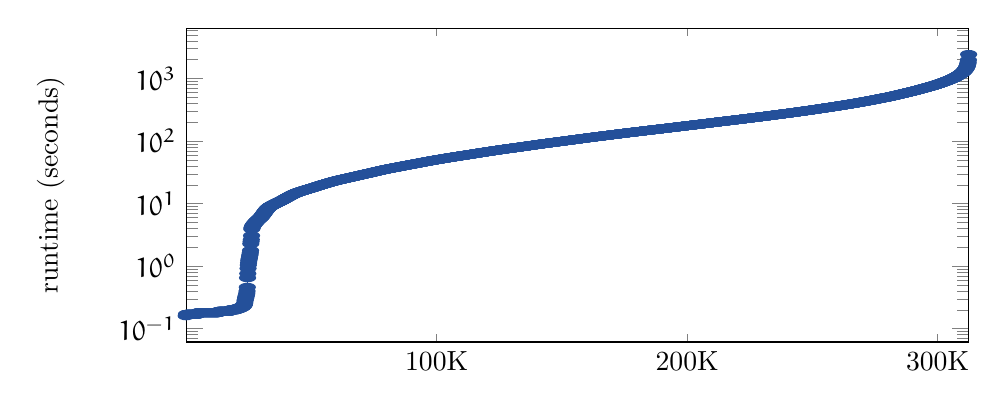
\begin{tikzpicture}
          \begin{axis}[xmin=1,xmax=312418, xtick={100000,200000,300000}, xticklabels={100K, 200K,300K}, scaled x ticks = false,ymode=log, yscale=0.7, xscale=1.45,ylabel={runtime (seconds)}]
          \addplot[color=colg, mark=*] coordinates {(1, 0.160) (101, 0.170) (201, 0.170) (301, 0.170) (401, 0.170) (501, 0.170) (601, 0.170) (701, 0.170) (801, 0.170) (901, 0.170) (1001, 0.170) (1101, 0.170) (1201, 0.170) (1301, 0.170) (1401, 0.170) (1501, 0.170) (1601, 0.170) (1701, 0.170) (1801, 0.170) (1901, 0.170) (2001, 0.170) (2101, 0.170) (2201, 0.170) (2301, 0.170) (2401, 0.170) (2501, 0.170) (2601, 0.170) (2701, 0.170) (2801, 0.170) (2901, 0.170) (3001, 0.170) (3101, 0.170) (3201, 0.170) (3301, 0.170) (3401, 0.170) (3501, 0.170) (3601, 0.170) (3701, 0.170) (3801, 0.170) (3901, 0.170) (4001, 0.170) (4101, 0.170) (4201, 0.170) (4301, 0.170) (4401, 0.170) (4501, 0.170) (4601, 0.170) (4701, 0.180) (4801, 0.180) (4901, 0.180) (5001, 0.180) (5101, 0.180) (5201, 0.180) (5301, 0.180) (5401, 0.180) (5501, 0.180) (5601, 0.180) (5701, 0.180) (5801, 0.180) (5901, 0.180) (6001, 0.180) (6101, 0.180) (6201, 0.180) (6301, 0.180) (6401, 0.180) (6501, 0.180) (6601, 0.180) (6701, 0.180) (6801, 0.180) (6901, 0.180) (7001, 0.180) (7101, 0.180) (7201, 0.180) (7301, 0.180) (7401, 0.180) (7501, 0.180) (7601, 0.180) (7701, 0.180) (7801, 0.180) (7901, 0.180) (8001, 0.180) (8101, 0.180) (8201, 0.180) (8301, 0.180) (8401, 0.180) (8501, 0.180) (8601, 0.180) (8701, 0.180) (8801, 0.180) (8901, 0.180) (9001, 0.180) (9101, 0.180) (9201, 0.180) (9301, 0.180) (9401, 0.180) (9501, 0.180) (9601, 0.180) (9701, 0.180) (9801, 0.180) (9901, 0.180) (10001, 0.180) (10101, 0.180) (10201, 0.180) (10301, 0.180) (10401, 0.180) (10501, 0.180) (10601, 0.180) (10701, 0.180) (10801, 0.180) (10901, 0.180) (11001, 0.180) (11101, 0.180) (11201, 0.180) (11301, 0.180) (11401, 0.180) (11501, 0.180) (11601, 0.180) (11701, 0.180) (11801, 0.180) (11901, 0.180) (12001, 0.180) (12101, 0.180) (12201, 0.180) (12301, 0.180) (12401, 0.180) (12501, 0.180) (12601, 0.180) (12701, 0.180) (12801, 0.180) (12901, 0.180) (13001, 0.190) (13101, 0.190) (13201, 0.190) (13301, 0.190) (13401, 0.190) (13501, 0.190) (13601, 0.190) (13701, 0.190) (13801, 0.190) (13901, 0.190) (14001, 0.190) (14101, 0.190) (14201, 0.190) (14301, 0.190) (14401, 0.190) (14501, 0.190) (14601, 0.190) (14701, 0.190) (14801, 0.190) (14901, 0.190) (15001, 0.190) (15101, 0.190) (15201, 0.190) (15301, 0.190) (15401, 0.190) (15501, 0.190) (15601, 0.190) (15701, 0.190) (15801, 0.190) (15901, 0.190) (16001, 0.190) (16101, 0.190) (16201, 0.190) (16301, 0.190) (16401, 0.190) (16501, 0.190) (16601, 0.190) (16701, 0.190) (16801, 0.190) (16901, 0.190) (17001, 0.190) (17101, 0.190) (17201, 0.190) (17301, 0.190) (17401, 0.190) (17501, 0.190) (17601, 0.200) (17701, 0.200) (17801, 0.200) (17901, 0.200) (18001, 0.200) (18101, 0.200) (18201, 0.200) (18301, 0.200) (18401, 0.200) (18501, 0.200) (18601, 0.200) (18701, 0.200) (18801, 0.200) (18901, 0.200) (19001, 0.200) (19101, 0.200) (19201, 0.200) (19301, 0.200) (19401, 0.200) (19501, 0.200) (19601, 0.200) (19701, 0.200) (19801, 0.200) (19901, 0.200) (20001, 0.200) (20101, 0.210) (20201, 0.210) (20301, 0.210) (20401, 0.210) (20501, 0.210) (20601, 0.210) (20701, 0.210) (20801, 0.210) (20901, 0.210) (21001, 0.210) (21101, 0.210) (21201, 0.210) (21301, 0.210) (21401, 0.210) (21501, 0.210) (21601, 0.220) (21701, 0.220) (21801, 0.220) (21901, 0.220) (22001, 0.220) (22101, 0.220) (22201, 0.220) (22301, 0.220) (22401, 0.220) (22501, 0.230) (22601, 0.230) (22701, 0.230) (22801, 0.230) (22901, 0.230) (23001, 0.240) (23101, 0.240) (23201, 0.240) (23301, 0.250) (23401, 0.260) (23501, 0.280) (23601, 0.290) (23701, 0.310) (23801, 0.310) (23901, 0.330) (24001, 0.340) (24101, 0.350) (24201, 0.370) (24301, 0.400) (24401, 0.460) (24501, 0.650) (24601, 0.760) (24701, 0.920) (24801, 1.040) (24901, 1.130) (25001, 1.220) (25101, 1.290) (25201, 1.340) (25301, 1.400) (25401, 1.480) (25501, 1.550) (25601, 1.640) (25701, 1.780) (25801, 2.280) (25901, 2.470) (26001, 2.650) (26101, 3.070) (26201, 3.920) (26301, 4.090) (26401, 4.220) (26501, 4.300) (26601, 4.380) (26701, 4.450) (26801, 4.520) (26901, 4.570) (27001, 4.630) (27101, 4.690) (27201, 4.740) (27301, 4.800) (27401, 4.850) (27501, 4.900) (27601, 4.950) (27701, 5.000) (27801, 5.050) (27901, 5.110) (28001, 5.160) (28101, 5.210) (28201, 5.260) (28301, 5.310) (28401, 5.360) (28501, 5.410) (28601, 5.450) (28701, 5.500) (28801, 5.540) (28901, 5.590) (29001, 5.630) (29101, 5.690) (29201, 5.740) (29301, 5.780) (29401, 5.830) (29501, 5.880) (29601, 5.930) (29701, 5.980) (29801, 6.050) (29901, 6.100) (30001, 6.160) (30101, 6.230) (30201, 6.320) (30301, 6.390) (30401, 6.450) (30501, 6.540) (30601, 6.630) (30701, 6.710) (30801, 6.800) (30901, 6.880) (31001, 6.970) (31101, 7.050) (31201, 7.150) (31301, 7.240) (31401, 7.350) (31501, 7.430) (31601, 7.530) (31701, 7.620) (31801, 7.710) (31901, 7.800) (32001, 7.900) (32101, 7.990) (32201, 8.080) (32301, 8.160) (32401, 8.250) (32501, 8.320) (32601, 8.410) (32701, 8.480) (32801, 8.540) (32901, 8.600) (33001, 8.670) (33101, 8.730) (33201, 8.790) (33301, 8.860) (33401, 8.920) (33501, 8.970) (33601, 9.030) (33701, 9.090) (33801, 9.140) (33901, 9.180) (34001, 9.230) (34101, 9.280) (34201, 9.330) (34301, 9.380) (34401, 9.420) (34501, 9.470) (34601, 9.510) (34701, 9.560) (34801, 9.600) (34901, 9.650) (35001, 9.690) (35101, 9.730) (35201, 9.780) (35301, 9.820) (35401, 9.870) (35501, 9.930) (35601, 9.980) (35701, 10.020) (35801, 10.070) (35901, 10.120) (36001, 10.170) (36101, 10.220) (36201, 10.270) (36301, 10.310) (36401, 10.360) (36501, 10.400) (36601, 10.430) (36701, 10.490) (36801, 10.530) (36901, 10.580) (37001, 10.620) (37101, 10.670) (37201, 10.710) (37301, 10.760) (37401, 10.800) (37501, 10.850) (37601, 10.910) (37701, 10.960) (37801, 11.010) (37901, 11.070) (38001, 11.120) (38101, 11.170) (38201, 11.220) (38301, 11.270) (38401, 11.330) (38501, 11.380) (38601, 11.440) (38701, 11.500) (38801, 11.560) (38901, 11.620) (39001, 11.680) (39101, 11.730) (39201, 11.790) (39301, 11.860) (39401, 11.930) (39501, 11.990) (39601, 12.060) (39701, 12.130) (39801, 12.190) (39901, 12.250) (40001, 12.310) (40101, 12.370) (40201, 12.430) (40301, 12.490) (40401, 12.560) (40501, 12.620) (40601, 12.680) (40701, 12.750) (40801, 12.820) (40901, 12.880) (41001, 12.940) (41101, 13.000) (41201, 13.060) (41301, 13.120) (41401, 13.200) (41501, 13.270) (41601, 13.340) (41701, 13.420) (41801, 13.480) (41901, 13.550) (42001, 13.620) (42101, 13.680) (42201, 13.740) (42301, 13.810) (42401, 13.860) (42501, 13.920) (42601, 13.990) (42701, 14.050) (42801, 14.120) (42901, 14.190) (43001, 14.240) (43101, 14.310) (43201, 14.350) (43301, 14.410) (43401, 14.470) (43501, 14.520) (43601, 14.580) (43701, 14.640) (43801, 14.700) (43901, 14.760) (44001, 14.810) (44101, 14.860) (44201, 14.910) (44301, 14.960) (44401, 15.010) (44501, 15.070) (44601, 15.120) (44701, 15.170) (44801, 15.220) (44901, 15.270) (45001, 15.330) (45101, 15.380) (45201, 15.410) (45301, 15.470) (45401, 15.520) (45501, 15.560) (45601, 15.610) (45701, 15.660) (45801, 15.710) (45901, 15.750) (46001, 15.800) (46101, 15.850) (46201, 15.900) (46301, 15.950) (46401, 15.980) (46501, 16.030) (46601, 16.080) (46701, 16.120) (46801, 16.170) (46901, 16.220) (47001, 16.270) (47101, 16.310) (47201, 16.350) (47301, 16.400) (47401, 16.440) (47501, 16.490) (47601, 16.540) (47701, 16.590) (47801, 16.640) (47901, 16.690) (48001, 16.740) (48101, 16.790) (48201, 16.830) (48301, 16.880) (48401, 16.920) (48501, 16.980) (48601, 17.010) (48701, 17.060) (48801, 17.110) (48901, 17.160) (49001, 17.210) (49101, 17.250) (49201, 17.300) (49301, 17.350) (49401, 17.420) (49501, 17.460) (49601, 17.500) (49701, 17.550) (49801, 17.600) (49901, 17.640) (50001, 17.700) (50101, 17.740) (50201, 17.790) (50301, 17.850) (50401, 17.890) (50501, 17.940) (50601, 17.990) (50701, 18.050) (50801, 18.100) (50901, 18.150) (51001, 18.200) (51101, 18.260) (51201, 18.320) (51301, 18.370) (51401, 18.430) (51501, 18.480) (51601, 18.530) (51701, 18.600) (51801, 18.650) (51901, 18.710) (52001, 18.770) (52101, 18.830) (52201, 18.880) (52301, 18.950) (52401, 19.000) (52501, 19.040) (52601, 19.110) (52701, 19.170) (52801, 19.220) (52901, 19.280) (53001, 19.330) (53101, 19.380) (53201, 19.450) (53301, 19.500) (53401, 19.560) (53501, 19.610) (53601, 19.670) (53701, 19.730) (53801, 19.800) (53901, 19.850) (54001, 19.910) (54101, 19.970) (54201, 20.030) (54301, 20.080) (54401, 20.140) (54501, 20.190) (54601, 20.250) (54701, 20.300) (54801, 20.360) (54901, 20.410) (55001, 20.450) (55101, 20.510) (55201, 20.560) (55301, 20.620) (55401, 20.670) (55501, 20.750) (55601, 20.810) (55701, 20.870) (55801, 20.920) (55901, 20.990) (56001, 21.040) (56101, 21.090) (56201, 21.160) (56301, 21.200) (56401, 21.260) (56501, 21.320) (56601, 21.390) (56701, 21.450) (56801, 21.510) (56901, 21.560) (57001, 21.630) (57101, 21.690) (57201, 21.750) (57301, 21.810) (57401, 21.870) (57501, 21.930) (57601, 21.980) (57701, 22.030) (57801, 22.080) (57901, 22.140) (58001, 22.200) (58101, 22.270) (58201, 22.330) (58301, 22.400) (58401, 22.460) (58501, 22.510) (58601, 22.560) (58701, 22.620) (58801, 22.680) (58901, 22.730) (59001, 22.790) (59101, 22.830) (59201, 22.890) (59301, 22.940) (59401, 23.000) (59501, 23.050) (59601, 23.100) (59701, 23.160) (59801, 23.210) (59901, 23.260) (60001, 23.320) (60101, 23.370) (60201, 23.440) (60301, 23.490) (60401, 23.530) (60501, 23.590) (60601, 23.650) (60701, 23.700) (60801, 23.760) (60901, 23.820) (61001, 23.880) (61101, 23.930) (61201, 23.980) (61301, 24.020) (61401, 24.070) (61501, 24.130) (61601, 24.180) (61701, 24.230) (61801, 24.280) (61901, 24.330) (62001, 24.380) (62101, 24.430) (62201, 24.480) (62301, 24.530) (62401, 24.590) (62501, 24.630) (62601, 24.680) (62701, 24.740) (62801, 24.790) (62901, 24.840) (63001, 24.890) (63101, 24.950) (63201, 25.000) (63301, 25.060) (63401, 25.110) (63501, 25.160) (63601, 25.210) (63701, 25.260) (63801, 25.300) (63901, 25.360) (64001, 25.420) (64101, 25.480) (64201, 25.530) (64301, 25.590) (64401, 25.640) (64501, 25.700) (64601, 25.740) (64701, 25.800) (64801, 25.850) (64901, 25.910) (65001, 25.970) (65101, 26.020) (65201, 26.060) (65301, 26.110) (65401, 26.170) (65501, 26.220) (65601, 26.280) (65701, 26.330) (65801, 26.380) (65901, 26.440) (66001, 26.500) (66101, 26.560) (66201, 26.620) (66301, 26.680) (66401, 26.730) (66501, 26.790) (66601, 26.850) (66701, 26.900) (66801, 26.950) (66901, 27.010) (67001, 27.060) (67101, 27.120) (67201, 27.180) (67301, 27.230) (67401, 27.280) (67501, 27.340) (67601, 27.400) (67701, 27.450) (67801, 27.510) (67901, 27.580) (68001, 27.630) (68101, 27.700) (68201, 27.760) (68301, 27.820) (68401, 27.880) (68501, 27.940) (68601, 27.980) (68701, 28.040) (68801, 28.090) (68901, 28.150) (69001, 28.200) (69101, 28.270) (69201, 28.340) (69301, 28.400) (69401, 28.460) (69501, 28.530) (69601, 28.590) (69701, 28.650) (69801, 28.710) (69901, 28.780) (70001, 28.840) (70101, 28.910) (70201, 28.970) (70301, 29.020) (70401, 29.080) (70501, 29.140) (70601, 29.210) (70701, 29.280) (70801, 29.340) (70901, 29.400) (71001, 29.460) (71101, 29.530) (71201, 29.580) (71301, 29.640) (71401, 29.700) (71501, 29.770) (71601, 29.830) (71701, 29.880) (71801, 29.950) (71901, 30.010) (72001, 30.060) (72101, 30.120) (72201, 30.190) (72301, 30.250) (72401, 30.310) (72501, 30.370) (72601, 30.430) (72701, 30.490) (72801, 30.550) (72901, 30.610) (73001, 30.670) (73101, 30.740) (73201, 30.800) (73301, 30.870) (73401, 30.930) (73501, 31.000) (73601, 31.060) (73701, 31.130) (73801, 31.190) (73901, 31.270) (74001, 31.330) (74101, 31.390) (74201, 31.450) (74301, 31.530) (74401, 31.610) (74501, 31.680) (74601, 31.750) (74701, 31.820) (74801, 31.900) (74901, 31.970) (75001, 32.040) (75101, 32.120) (75201, 32.180) (75301, 32.250) (75401, 32.320) (75501, 32.390) (75601, 32.450) (75701, 32.520) (75801, 32.600) (75901, 32.680) (76001, 32.760) (76101, 32.820) (76201, 32.880) (76301, 32.950) (76401, 33.020) (76501, 33.080) (76601, 33.160) (76701, 33.230) (76801, 33.300) (76901, 33.370) (77001, 33.450) (77101, 33.510) (77201, 33.590) (77301, 33.670) (77401, 33.730) (77501, 33.810) (77601, 33.890) (77701, 33.960) (77801, 34.030) (77901, 34.100) (78001, 34.170) (78101, 34.230) (78201, 34.300) (78301, 34.360) (78401, 34.440) (78501, 34.510) (78601, 34.580) (78701, 34.650) (78801, 34.710) (78901, 34.790) (79001, 34.860) (79101, 34.920) (79201, 35.000) (79301, 35.080) (79401, 35.140) (79501, 35.210) (79601, 35.280) (79701, 35.350) (79801, 35.420) (79901, 35.480) (80001, 35.540) (80101, 35.610) (80201, 35.690) (80301, 35.760) (80401, 35.820) (80501, 35.870) (80601, 35.930) (80701, 35.990) (80801, 36.060) (80901, 36.130) (81001, 36.200) (81101, 36.260) (81201, 36.320) (81301, 36.390) (81401, 36.450) (81501, 36.530) (81601, 36.590) (81701, 36.650) (81801, 36.710) (81901, 36.790) (82001, 36.850) (82101, 36.920) (82201, 36.990) (82301, 37.040) (82401, 37.120) (82501, 37.190) (82601, 37.250) (82701, 37.320) (82801, 37.390) (82901, 37.450) (83001, 37.520) (83101, 37.600) (83201, 37.660) (83301, 37.720) (83401, 37.770) (83501, 37.830) (83601, 37.900) (83701, 37.980) (83801, 38.030) (83901, 38.100) (84001, 38.180) (84101, 38.250) (84201, 38.330) (84301, 38.400) (84401, 38.450) (84501, 38.510) (84601, 38.570) (84701, 38.630) (84801, 38.690) (84901, 38.760) (85001, 38.850) (85101, 38.910) (85201, 38.980) (85301, 39.060) (85401, 39.120) (85501, 39.200) (85601, 39.280) (85701, 39.350) (85801, 39.410) (85901, 39.480) (86001, 39.550) (86101, 39.620) (86201, 39.690) (86301, 39.750) (86401, 39.830) (86501, 39.900) (86601, 39.970) (86701, 40.040) (86801, 40.100) (86901, 40.170) (87001, 40.240) (87101, 40.300) (87201, 40.380) (87301, 40.450) (87401, 40.520) (87501, 40.600) (87601, 40.670) (87701, 40.750) (87801, 40.820) (87901, 40.880) (88001, 40.950) (88101, 41.010) (88201, 41.090) (88301, 41.150) (88401, 41.220) (88501, 41.290) (88601, 41.360) (88701, 41.440) (88801, 41.510) (88901, 41.580) (89001, 41.650) (89101, 41.740) (89201, 41.820) (89301, 41.900) (89401, 41.960) (89501, 42.030) (89601, 42.100) (89701, 42.180) (89801, 42.250) (89901, 42.320) (90001, 42.400) (90101, 42.470) (90201, 42.540) (90301, 42.620) (90401, 42.690) (90501, 42.760) (90601, 42.820) (90701, 42.890) (90801, 42.970) (90901, 43.040) (91001, 43.110) (91101, 43.190) (91201, 43.260) (91301, 43.330) (91401, 43.410) (91501, 43.490) (91601, 43.560) (91701, 43.640) (91801, 43.700) (91901, 43.780) (92001, 43.860) (92101, 43.930) (92201, 44.000) (92301, 44.090) (92401, 44.170) (92501, 44.240) (92601, 44.310) (92701, 44.390) (92801, 44.470) (92901, 44.550) (93001, 44.630) (93101, 44.700) (93201, 44.780) (93301, 44.870) (93401, 44.950) (93501, 45.020) (93601, 45.100) (93701, 45.200) (93801, 45.270) (93901, 45.340) (94001, 45.420) (94101, 45.530) (94201, 45.610) (94301, 45.690) (94401, 45.770) (94501, 45.850) (94601, 45.940) (94701, 46.020) (94801, 46.100) (94901, 46.180) (95001, 46.240) (95101, 46.330) (95201, 46.400) (95301, 46.480) (95401, 46.570) (95501, 46.650) (95601, 46.720) (95701, 46.800) (95801, 46.880) (95901, 46.960) (96001, 47.030) (96101, 47.100) (96201, 47.170) (96301, 47.260) (96401, 47.340) (96501, 47.430) (96601, 47.500) (96701, 47.590) (96801, 47.670) (96901, 47.760) (97001, 47.840) (97101, 47.920) (97201, 48.000) (97301, 48.100) (97401, 48.180) (97501, 48.270) (97601, 48.340) (97701, 48.430) (97801, 48.520) (97901, 48.590) (98001, 48.660) (98101, 48.740) (98201, 48.800) (98301, 48.890) (98401, 48.980) (98501, 49.060) (98601, 49.150) (98701, 49.230) (98801, 49.310) (98901, 49.390) (99001, 49.480) (99101, 49.540) (99201, 49.610) (99301, 49.700) (99401, 49.780) (99501, 49.860) (99601, 49.930) (99701, 50.010) (99801, 50.100) (99901, 50.180) (100001, 50.250) (100101, 50.320) (100201, 50.410) (100301, 50.490) (100401, 50.570) (100501, 50.650) (100601, 50.710) (100701, 50.790) (100801, 50.870) (100901, 50.940) (101001, 51.020) (101101, 51.100) (101201, 51.190) (101301, 51.260) (101401, 51.350) (101501, 51.430) (101601, 51.500) (101701, 51.590) (101801, 51.670) (101901, 51.750) (102001, 51.830) (102101, 51.920) (102201, 51.990) (102301, 52.080) (102401, 52.170) (102501, 52.260) (102601, 52.340) (102701, 52.420) (102801, 52.500) (102901, 52.580) (103001, 52.660) (103101, 52.750) (103201, 52.830) (103301, 52.920) (103401, 53.000) (103501, 53.080) (103601, 53.160) (103701, 53.240) (103801, 53.320) (103901, 53.410) (104001, 53.490) (104101, 53.570) (104201, 53.640) (104301, 53.730) (104401, 53.820) (104501, 53.900) (104601, 53.970) (104701, 54.040) (104801, 54.120) (104901, 54.210) (105001, 54.280) (105101, 54.350) (105201, 54.440) (105301, 54.510) (105401, 54.610) (105501, 54.700) (105601, 54.770) (105701, 54.850) (105801, 54.930) (105901, 55.010) (106001, 55.100) (106101, 55.180) (106201, 55.270) (106301, 55.350) (106401, 55.430) (106501, 55.500) (106601, 55.580) (106701, 55.670) (106801, 55.750) (106901, 55.820) (107001, 55.890) (107101, 55.960) (107201, 56.070) (107301, 56.160) (107401, 56.240) (107501, 56.320) (107601, 56.400) (107701, 56.480) (107801, 56.570) (107901, 56.660) (108001, 56.730) (108101, 56.820) (108201, 56.910) (108301, 56.980) (108401, 57.070) (108501, 57.160) (108601, 57.240) (108701, 57.320) (108801, 57.410) (108901, 57.500) (109001, 57.590) (109101, 57.670) (109201, 57.770) (109301, 57.840) (109401, 57.920) (109501, 58.000) (109601, 58.080) (109701, 58.170) (109801, 58.250) (109901, 58.340) (110001, 58.410) (110101, 58.490) (110201, 58.560) (110301, 58.640) (110401, 58.710) (110501, 58.790) (110601, 58.860) (110701, 58.950) (110801, 59.050) (110901, 59.130) (111001, 59.210) (111101, 59.280) (111201, 59.380) (111301, 59.470) (111401, 59.570) (111501, 59.650) (111601, 59.740) (111701, 59.820) (111801, 59.900) (111901, 59.990) (112001, 60.060) (112101, 60.140) (112201, 60.220) (112301, 60.300) (112401, 60.400) (112501, 60.470) (112601, 60.550) (112701, 60.640) (112801, 60.720) (112901, 60.820) (113001, 60.910) (113101, 60.980) (113201, 61.070) (113301, 61.170) (113401, 61.250) (113501, 61.350) (113601, 61.450) (113701, 61.550) (113801, 61.620) (113901, 61.720) (114001, 61.800) (114101, 61.900) (114201, 61.990) (114301, 62.070) (114401, 62.160) (114501, 62.270) (114601, 62.360) (114701, 62.440) (114801, 62.540) (114901, 62.640) (115001, 62.740) (115101, 62.830) (115201, 62.920) (115301, 63.010) (115401, 63.100) (115501, 63.210) (115601, 63.320) (115701, 63.420) (115801, 63.510) (115901, 63.610) (116001, 63.710) (116101, 63.800) (116201, 63.880) (116301, 63.980) (116401, 64.070) (116501, 64.140) (116601, 64.230) (116701, 64.310) (116801, 64.400) (116901, 64.490) (117001, 64.590) (117101, 64.690) (117201, 64.790) (117301, 64.870) (117401, 64.960) (117501, 65.050) (117601, 65.150) (117701, 65.230) (117801, 65.320) (117901, 65.410) (118001, 65.500) (118101, 65.590) (118201, 65.680) (118301, 65.790) (118401, 65.890) (118501, 65.990) (118601, 66.090) (118701, 66.200) (118801, 66.290) (118901, 66.390) (119001, 66.490) (119101, 66.580) (119201, 66.680) (119301, 66.760) (119401, 66.850) (119501, 66.950) (119601, 67.050) (119701, 67.150) (119801, 67.250) (119901, 67.360) (120001, 67.440) (120101, 67.540) (120201, 67.630) (120301, 67.740) (120401, 67.840) (120501, 67.940) (120601, 68.030) (120701, 68.120) (120801, 68.220) (120901, 68.330) (121001, 68.420) (121101, 68.510) (121201, 68.610) (121301, 68.710) (121401, 68.790) (121501, 68.880) (121601, 68.970) (121701, 69.080) (121801, 69.170) (121901, 69.250) (122001, 69.340) (122101, 69.430) (122201, 69.510) (122301, 69.600) (122401, 69.700) (122501, 69.790) (122601, 69.890) (122701, 70.010) (122801, 70.120) (122901, 70.230) (123001, 70.310) (123101, 70.410) (123201, 70.510) (123301, 70.610) (123401, 70.700) (123501, 70.790) (123601, 70.890) (123701, 70.980) (123801, 71.060) (123901, 71.180) (124001, 71.290) (124101, 71.390) (124201, 71.470) (124301, 71.560) (124401, 71.640) (124501, 71.730) (124601, 71.830) (124701, 71.940) (124801, 72.030) (124901, 72.150) (125001, 72.230) (125101, 72.350) (125201, 72.460) (125301, 72.550) (125401, 72.650) (125501, 72.740) (125601, 72.830) (125701, 72.930) (125801, 73.030) (125901, 73.110) (126001, 73.220) (126101, 73.320) (126201, 73.440) (126301, 73.530) (126401, 73.640) (126501, 73.740) (126601, 73.850) (126701, 73.930) (126801, 74.030) (126901, 74.120) (127001, 74.220) (127101, 74.320) (127201, 74.420) (127301, 74.500) (127401, 74.600) (127501, 74.700) (127601, 74.800) (127701, 74.890) (127801, 75.000) (127901, 75.090) (128001, 75.190) (128101, 75.300) (128201, 75.400) (128301, 75.490) (128401, 75.590) (128501, 75.680) (128601, 75.770) (128701, 75.860) (128801, 75.950) (128901, 76.050) (129001, 76.130) (129101, 76.230) (129201, 76.310) (129301, 76.420) (129401, 76.520) (129501, 76.620) (129601, 76.720) (129701, 76.800) (129801, 76.900) (129901, 76.990) (130001, 77.090) (130101, 77.170) (130201, 77.270) (130301, 77.360) (130401, 77.460) (130501, 77.550) (130601, 77.650) (130701, 77.750) (130801, 77.850) (130901, 77.950) (131001, 78.050) (131101, 78.130) (131201, 78.220) (131301, 78.330) (131401, 78.430) (131501, 78.530) (131601, 78.640) (131701, 78.750) (131801, 78.850) (131901, 78.960) (132001, 79.070) (132101, 79.150) (132201, 79.250) (132301, 79.350) (132401, 79.450) (132501, 79.550) (132601, 79.650) (132701, 79.740) (132801, 79.860) (132901, 79.960) (133001, 80.060) (133101, 80.160) (133201, 80.270) (133301, 80.380) (133401, 80.490) (133501, 80.600) (133601, 80.690) (133701, 80.800) (133801, 80.910) (133901, 81.030) (134001, 81.120) (134101, 81.240) (134201, 81.340) (134301, 81.440) (134401, 81.530) (134501, 81.630) (134601, 81.740) (134701, 81.850) (134801, 81.970) (134901, 82.080) (135001, 82.210) (135101, 82.320) (135201, 82.430) (135301, 82.520) (135401, 82.620) (135501, 82.730) (135601, 82.850) (135701, 82.950) (135801, 83.080) (135901, 83.180) (136001, 83.280) (136101, 83.380) (136201, 83.500) (136301, 83.610) (136401, 83.720) (136501, 83.840) (136601, 83.950) (136701, 84.050) (136801, 84.150) (136901, 84.250) (137001, 84.350) (137101, 84.470) (137201, 84.570) (137301, 84.690) (137401, 84.790) (137501, 84.890) (137601, 85.020) (137701, 85.110) (137801, 85.220) (137901, 85.320) (138001, 85.440) (138101, 85.550) (138201, 85.660) (138301, 85.770) (138401, 85.900) (138501, 86.010) (138601, 86.110) (138701, 86.220) (138801, 86.350) (138901, 86.480) (139001, 86.610) (139101, 86.710) (139201, 86.830) (139301, 86.940) (139401, 87.070) (139501, 87.170) (139601, 87.280) (139701, 87.410) (139801, 87.530) (139901, 87.650) (140001, 87.740) (140101, 87.880) (140201, 88.000) (140301, 88.100) (140401, 88.210) (140501, 88.340) (140601, 88.460) (140701, 88.590) (140801, 88.700) (140901, 88.820) (141001, 88.910) (141101, 89.040) (141201, 89.160) (141301, 89.270) (141401, 89.400) (141501, 89.520) (141601, 89.610) (141701, 89.710) (141801, 89.820) (141901, 89.940) (142001, 90.050) (142101, 90.150) (142201, 90.270) (142301, 90.390) (142401, 90.490) (142501, 90.590) (142601, 90.700) (142701, 90.810) (142801, 90.950) (142901, 91.060) (143001, 91.170) (143101, 91.290) (143201, 91.400) (143301, 91.510) (143401, 91.630) (143501, 91.740) (143601, 91.860) (143701, 91.980) (143801, 92.100) (143901, 92.210) (144001, 92.310) (144101, 92.410) (144201, 92.520) (144301, 92.630) (144401, 92.730) (144501, 92.850) (144601, 92.960) (144701, 93.080) (144801, 93.200) (144901, 93.300) (145001, 93.440) (145101, 93.520) (145201, 93.630) (145301, 93.750) (145401, 93.870) (145501, 93.990) (145601, 94.120) (145701, 94.230) (145801, 94.340) (145901, 94.470) (146001, 94.590) (146101, 94.700) (146201, 94.820) (146301, 94.910) (146401, 95.030) (146501, 95.130) (146601, 95.250) (146701, 95.350) (146801, 95.470) (146901, 95.590) (147001, 95.730) (147101, 95.830) (147201, 95.950) (147301, 96.060) (147401, 96.200) (147501, 96.290) (147601, 96.400) (147701, 96.550) (147801, 96.670) (147901, 96.800) (148001, 96.920) (148101, 97.020) (148201, 97.130) (148301, 97.250) (148401, 97.340) (148501, 97.460) (148601, 97.580) (148701, 97.700) (148801, 97.830) (148901, 97.950) (149001, 98.070) (149101, 98.190) (149201, 98.310) (149301, 98.430) (149401, 98.530) (149501, 98.630) (149601, 98.770) (149701, 98.880) (149801, 99.000) (149901, 99.130) (150001, 99.240) (150101, 99.360) (150201, 99.480) (150301, 99.580) (150401, 99.700) (150501, 99.820) (150601, 99.940) (150701, 100.070) (150801, 100.210) (150901, 100.340) (151001, 100.480) (151101, 100.600) (151201, 100.720) (151301, 100.840) (151401, 100.980) (151501, 101.130) (151601, 101.240) (151701, 101.360) (151801, 101.500) (151901, 101.620) (152001, 101.740) (152101, 101.860) (152201, 101.980) (152301, 102.100) (152401, 102.230) (152501, 102.360) (152601, 102.490) (152701, 102.620) (152801, 102.750) (152901, 102.870) (153001, 103.000) (153101, 103.120) (153201, 103.230) (153301, 103.350) (153401, 103.490) (153501, 103.610) (153601, 103.750) (153701, 103.880) (153801, 104.000) (153901, 104.130) (154001, 104.260) (154101, 104.360) (154201, 104.470) (154301, 104.590) (154401, 104.720) (154501, 104.840) (154601, 104.980) (154701, 105.100) (154801, 105.230) (154901, 105.380) (155001, 105.490) (155101, 105.620) (155201, 105.720) (155301, 105.860) (155401, 106.000) (155501, 106.140) (155601, 106.270) (155701, 106.420) (155801, 106.550) (155901, 106.710) (156001, 106.830) (156101, 106.970) (156201, 107.100) (156301, 107.230) (156401, 107.360) (156501, 107.490) (156601, 107.620) (156701, 107.770) (156801, 107.890) (156901, 108.040) (157001, 108.180) (157101, 108.320) (157201, 108.450) (157301, 108.590) (157401, 108.700) (157501, 108.830) (157601, 108.970) (157701, 109.080) (157801, 109.220) (157901, 109.360) (158001, 109.490) (158101, 109.630) (158201, 109.770) (158301, 109.900) (158401, 110.030) (158501, 110.170) (158601, 110.290) (158701, 110.430) (158801, 110.550) (158901, 110.700) (159001, 110.850) (159101, 111.000) (159201, 111.130) (159301, 111.260) (159401, 111.410) (159501, 111.570) (159601, 111.720) (159701, 111.850) (159801, 111.990) (159901, 112.140) (160001, 112.290) (160101, 112.390) (160201, 112.530) (160301, 112.670) (160401, 112.800) (160501, 112.920) (160601, 113.070) (160701, 113.240) (160801, 113.360) (160901, 113.490) (161001, 113.630) (161101, 113.770) (161201, 113.890) (161301, 114.020) (161401, 114.170) (161501, 114.300) (161601, 114.450) (161701, 114.570) (161801, 114.700) (161901, 114.840) (162001, 114.960) (162101, 115.080) (162201, 115.210) (162301, 115.360) (162401, 115.520) (162501, 115.660) (162601, 115.800) (162701, 115.970) (162801, 116.090) (162901, 116.220) (163001, 116.370) (163101, 116.500) (163201, 116.630) (163301, 116.770) (163401, 116.900) (163501, 117.050) (163601, 117.200) (163701, 117.350) (163801, 117.500) (163901, 117.600) (164001, 117.740) (164101, 117.860) (164201, 118.000) (164301, 118.150) (164401, 118.270) (164501, 118.420) (164601, 118.550) (164701, 118.680) (164801, 118.840) (164901, 118.980) (165001, 119.140) (165101, 119.280) (165201, 119.420) (165301, 119.550) (165401, 119.720) (165501, 119.840) (165601, 119.960) (165701, 120.110) (165801, 120.240) (165901, 120.370) (166001, 120.500) (166101, 120.620) (166201, 120.740) (166301, 120.880) (166401, 121.020) (166501, 121.160) (166601, 121.290) (166701, 121.450) (166801, 121.580) (166901, 121.730) (167001, 121.880) (167101, 122.000) (167201, 122.140) (167301, 122.300) (167401, 122.440) (167501, 122.590) (167601, 122.690) (167701, 122.830) (167801, 122.970) (167901, 123.140) (168001, 123.310) (168101, 123.460) (168201, 123.610) (168301, 123.730) (168401, 123.880) (168501, 124.010) (168601, 124.170) (168701, 124.330) (168801, 124.470) (168901, 124.640) (169001, 124.800) (169101, 124.910) (169201, 125.040) (169301, 125.200) (169401, 125.360) (169501, 125.510) (169601, 125.660) (169701, 125.780) (169801, 125.930) (169901, 126.060) (170001, 126.200) (170101, 126.370) (170201, 126.530) (170301, 126.670) (170401, 126.840) (170501, 127.010) (170601, 127.140) (170701, 127.280) (170801, 127.420) (170901, 127.580) (171001, 127.690) (171101, 127.840) (171201, 128.010) (171301, 128.170) (171401, 128.290) (171501, 128.430) (171601, 128.590) (171701, 128.750) (171801, 128.900) (171901, 129.070) (172001, 129.210) (172101, 129.350) (172201, 129.500) (172301, 129.660) (172401, 129.820) (172501, 129.960) (172601, 130.090) (172701, 130.220) (172801, 130.350) (172901, 130.510) (173001, 130.620) (173101, 130.760) (173201, 130.930) (173301, 131.100) (173401, 131.230) (173501, 131.410) (173601, 131.570) (173701, 131.700) (173801, 131.890) (173901, 132.050) (174001, 132.190) (174101, 132.350) (174201, 132.520) (174301, 132.680) (174401, 132.810) (174501, 132.960) (174601, 133.140) (174701, 133.300) (174801, 133.440) (174901, 133.600) (175001, 133.750) (175101, 133.900) (175201, 134.050) (175301, 134.180) (175401, 134.320) (175501, 134.490) (175601, 134.620) (175701, 134.780) (175801, 134.930) (175901, 135.060) (176001, 135.210) (176101, 135.350) (176201, 135.490) (176301, 135.650) (176401, 135.830) (176501, 135.980) (176601, 136.150) (176701, 136.320) (176801, 136.460) (176901, 136.610) (177001, 136.790) (177101, 136.950) (177201, 137.090) (177301, 137.230) (177401, 137.380) (177501, 137.540) (177601, 137.690) (177701, 137.820) (177801, 137.960) (177901, 138.090) (178001, 138.230) (178101, 138.380) (178201, 138.520) (178301, 138.680) (178401, 138.820) (178501, 138.970) (178601, 139.150) (178701, 139.320) (178801, 139.480) (178901, 139.640) (179001, 139.790) (179101, 139.940) (179201, 140.110) (179301, 140.270) (179401, 140.400) (179501, 140.550) (179601, 140.710) (179701, 140.880) (179801, 141.010) (179901, 141.200) (180001, 141.360) (180101, 141.530) (180201, 141.670) (180301, 141.830) (180401, 142.000) (180501, 142.150) (180601, 142.310) (180701, 142.490) (180801, 142.650) (180901, 142.790) (181001, 142.940) (181101, 143.080) (181201, 143.220) (181301, 143.370) (181401, 143.530) (181501, 143.680) (181601, 143.830) (181701, 144.010) (181801, 144.160) (181901, 144.310) (182001, 144.460) (182101, 144.630) (182201, 144.760) (182301, 144.920) (182401, 145.070) (182501, 145.210) (182601, 145.350) (182701, 145.530) (182801, 145.700) (182901, 145.850) (183001, 146.040) (183101, 146.190) (183201, 146.370) (183301, 146.550) (183401, 146.710) (183501, 146.860) (183601, 147.030) (183701, 147.190) (183801, 147.330) (183901, 147.490) (184001, 147.630) (184101, 147.810) (184201, 147.980) (184301, 148.120) (184401, 148.300) (184501, 148.470) (184601, 148.620) (184701, 148.790) (184801, 149.000) (184901, 149.150) (185001, 149.300) (185101, 149.500) (185201, 149.700) (185301, 149.870) (185401, 150.010) (185501, 150.160) (185601, 150.330) (185701, 150.460) (185801, 150.620) (185901, 150.790) (186001, 150.940) (186101, 151.090) (186201, 151.240) (186301, 151.390) (186401, 151.560) (186501, 151.720) (186601, 151.860) (186701, 152.040) (186801, 152.210) (186901, 152.370) (187001, 152.510) (187101, 152.690) (187201, 152.850) (187301, 153.030) (187401, 153.180) (187501, 153.360) (187601, 153.540) (187701, 153.720) (187801, 153.910) (187901, 154.090) (188001, 154.250) (188101, 154.440) (188201, 154.600) (188301, 154.790) (188401, 154.970) (188501, 155.140) (188601, 155.340) (188701, 155.500) (188801, 155.650) (188901, 155.820) (189001, 155.950) (189101, 156.130) (189201, 156.300) (189301, 156.470) (189401, 156.640) (189501, 156.800) (189601, 156.960) (189701, 157.130) (189801, 157.260) (189901, 157.430) (190001, 157.600) (190101, 157.750) (190201, 157.920) (190301, 158.080) (190401, 158.250) (190501, 158.440) (190601, 158.600) (190701, 158.790) (190801, 158.950) (190901, 159.120) (191001, 159.300) (191101, 159.450) (191201, 159.620) (191301, 159.770) (191401, 159.980) (191501, 160.170) (191601, 160.370) (191701, 160.590) (191801, 160.760) (191901, 160.940) (192001, 161.140) (192101, 161.320) (192201, 161.510) (192301, 161.720) (192401, 161.880) (192501, 162.080) (192601, 162.270) (192701, 162.440) (192801, 162.620) (192901, 162.860) (193001, 163.050) (193101, 163.220) (193201, 163.370) (193301, 163.580) (193401, 163.750) (193501, 163.900) (193601, 164.070) (193701, 164.220) (193801, 164.380) (193901, 164.570) (194001, 164.730) (194101, 164.930) (194201, 165.100) (194301, 165.260) (194401, 165.450) (194501, 165.640) (194601, 165.850) (194701, 166.040) (194801, 166.260) (194901, 166.420) (195001, 166.590) (195101, 166.760) (195201, 166.950) (195301, 167.110) (195401, 167.270) (195501, 167.440) (195601, 167.640) (195701, 167.800) (195801, 168.020) (195901, 168.180) (196001, 168.390) (196101, 168.570) (196201, 168.740) (196301, 168.940) (196401, 169.140) (196501, 169.340) (196601, 169.550) (196701, 169.750) (196801, 169.990) (196901, 170.200) (197001, 170.390) (197101, 170.570) (197201, 170.800) (197301, 170.990) (197401, 171.160) (197501, 171.370) (197601, 171.550) (197701, 171.760) (197801, 171.980) (197901, 172.170) (198001, 172.380) (198101, 172.560) (198201, 172.750) (198301, 172.940) (198401, 173.140) (198501, 173.320) (198601, 173.520) (198701, 173.690) (198801, 173.890) (198901, 174.100) (199001, 174.290) (199101, 174.470) (199201, 174.670) (199301, 174.880) (199401, 175.080) (199501, 175.270) (199601, 175.460) (199701, 175.630) (199801, 175.840) (199901, 176.020) (200001, 176.190) (200101, 176.380) (200201, 176.590) (200301, 176.770) (200401, 176.940) (200501, 177.150) (200601, 177.380) (200701, 177.550) (200801, 177.740) (200901, 177.950) (201001, 178.140) (201101, 178.330) (201201, 178.510) (201301, 178.720) (201401, 178.900) (201501, 179.090) (201601, 179.240) (201701, 179.440) (201801, 179.630) (201901, 179.820) (202001, 180.020) (202101, 180.210) (202201, 180.390) (202301, 180.590) (202401, 180.790) (202501, 181.000) (202601, 181.200) (202701, 181.420) (202801, 181.630) (202901, 181.800) (203001, 182.010) (203101, 182.240) (203201, 182.440) (203301, 182.650) (203401, 182.820) (203501, 182.990) (203601, 183.190) (203701, 183.360) (203801, 183.570) (203901, 183.730) (204001, 183.930) (204101, 184.130) (204201, 184.320) (204301, 184.530) (204401, 184.750) (204501, 184.980) (204601, 185.230) (204701, 185.430) (204801, 185.620) (204901, 185.870) (205001, 186.110) (205101, 186.290) (205201, 186.480) (205301, 186.720) (205401, 186.930) (205501, 187.160) (205601, 187.370) (205701, 187.590) (205801, 187.810) (205901, 188.010) (206001, 188.200) (206101, 188.430) (206201, 188.610) (206301, 188.820) (206401, 189.070) (206501, 189.300) (206601, 189.480) (206701, 189.700) (206801, 189.880) (206901, 190.070) (207001, 190.300) (207101, 190.550) (207201, 190.700) (207301, 190.920) (207401, 191.120) (207501, 191.310) (207601, 191.540) (207701, 191.770) (207801, 191.970) (207901, 192.150) (208001, 192.390) (208101, 192.610) (208201, 192.880) (208301, 193.070) (208401, 193.300) (208501, 193.520) (208601, 193.730) (208701, 193.950) (208801, 194.190) (208901, 194.420) (209001, 194.640) (209101, 194.840) (209201, 195.100) (209301, 195.320) (209401, 195.490) (209501, 195.670) (209601, 195.900) (209701, 196.100) (209801, 196.350) (209901, 196.580) (210001, 196.800) (210101, 197.050) (210201, 197.290) (210301, 197.540) (210401, 197.740) (210501, 197.950) (210601, 198.150) (210701, 198.380) (210801, 198.600) (210901, 198.830) (211001, 199.060) (211101, 199.280) (211201, 199.500) (211301, 199.720) (211401, 199.980) (211501, 200.210) (211601, 200.470) (211701, 200.710) (211801, 200.940) (211901, 201.150) (212001, 201.380) (212101, 201.610) (212201, 201.830) (212301, 202.060) (212401, 202.300) (212501, 202.520) (212601, 202.710) (212701, 202.940) (212801, 203.160) (212901, 203.400) (213001, 203.590) (213101, 203.840) (213201, 204.120) (213301, 204.310) (213401, 204.510) (213501, 204.730) (213601, 204.980) (213701, 205.190) (213801, 205.390) (213901, 205.630) (214001, 205.890) (214101, 206.090) (214201, 206.320) (214301, 206.540) (214401, 206.760) (214501, 206.970) (214601, 207.190) (214701, 207.450) (214801, 207.640) (214901, 207.850) (215001, 208.070) (215101, 208.330) (215201, 208.620) (215301, 208.880) (215401, 209.100) (215501, 209.330) (215601, 209.550) (215701, 209.730) (215801, 210.000) (215901, 210.240) (216001, 210.470) (216101, 210.660) (216201, 210.880) (216301, 211.110) (216401, 211.370) (216501, 211.620) (216601, 211.840) (216701, 212.070) (216801, 212.320) (216901, 212.530) (217001, 212.740) (217101, 212.960) (217201, 213.230) (217301, 213.460) (217401, 213.680) (217501, 213.900) (217601, 214.140) (217701, 214.380) (217801, 214.630) (217901, 214.890) (218001, 215.110) (218101, 215.320) (218201, 215.570) (218301, 215.830) (218401, 216.050) (218501, 216.350) (218601, 216.620) (218701, 216.860) (218801, 217.140) (218901, 217.410) (219001, 217.630) (219101, 217.860) (219201, 218.130) (219301, 218.360) (219401, 218.600) (219501, 218.850) (219601, 219.080) (219701, 219.320) (219801, 219.530) (219901, 219.760) (220001, 219.980) (220101, 220.230) (220201, 220.470) (220301, 220.700) (220401, 220.940) (220501, 221.150) (220601, 221.380) (220701, 221.590) (220801, 221.820) (220901, 222.080) (221001, 222.350) (221101, 222.610) (221201, 222.820) (221301, 223.040) (221401, 223.300) (221501, 223.550) (221601, 223.850) (221701, 224.110) (221801, 224.350) (221901, 224.620) (222001, 224.930) (222101, 225.190) (222201, 225.450) (222301, 225.720) (222401, 226.000) (222501, 226.280) (222601, 226.530) (222701, 226.820) (222801, 227.070) (222901, 227.370) (223001, 227.610) (223101, 227.870) (223201, 228.110) (223301, 228.370) (223401, 228.560) (223501, 228.820) (223601, 229.060) (223701, 229.310) (223801, 229.570) (223901, 229.830) (224001, 230.140) (224101, 230.410) (224201, 230.680) (224301, 230.930) (224401, 231.210) (224501, 231.460) (224601, 231.680) (224701, 231.960) (224801, 232.250) (224901, 232.480) (225001, 232.760) (225101, 233.010) (225201, 233.270) (225301, 233.550) (225401, 233.820) (225501, 234.060) (225601, 234.350) (225701, 234.610) (225801, 234.930) (225901, 235.160) (226001, 235.420) (226101, 235.720) (226201, 236.000) (226301, 236.320) (226401, 236.640) (226501, 236.890) (226601, 237.130) (226701, 237.400) (226801, 237.720) (226901, 238.010) (227001, 238.260) (227101, 238.550) (227201, 238.870) (227301, 239.140) (227401, 239.420) (227501, 239.700) (227601, 239.990) (227701, 240.280) (227801, 240.520) (227901, 240.770) (228001, 241.050) (228101, 241.310) (228201, 241.590) (228301, 241.830) (228401, 242.130) (228501, 242.410) (228601, 242.650) (228701, 242.950) (228801, 243.240) (228901, 243.580) (229001, 243.820) (229101, 244.100) (229201, 244.360) (229301, 244.640) (229401, 244.900) (229501, 245.190) (229601, 245.480) (229701, 245.760) (229801, 246.020) (229901, 246.320) (230001, 246.590) (230101, 246.920) (230201, 247.180) (230301, 247.470) (230401, 247.780) (230501, 248.070) (230601, 248.350) (230701, 248.660) (230801, 248.980) (230901, 249.270) (231001, 249.540) (231101, 249.860) (231201, 250.170) (231301, 250.460) (231401, 250.770) (231501, 251.050) (231601, 251.300) (231701, 251.570) (231801, 251.840) (231901, 252.140) (232001, 252.460) (232101, 252.760) (232201, 253.100) (232301, 253.360) (232401, 253.680) (232501, 253.950) (232601, 254.240) (232701, 254.560) (232801, 254.850) (232901, 255.160) (233001, 255.500) (233101, 255.770) (233201, 256.100) (233301, 256.420) (233401, 256.820) (233501, 257.220) (233601, 257.510) (233701, 257.790) (233801, 258.080) (233901, 258.400) (234001, 258.700) (234101, 258.990) (234201, 259.270) (234301, 259.610) (234401, 260.000) (234501, 260.280) (234601, 260.580) (234701, 260.910) (234801, 261.260) (234901, 261.610) (235001, 261.850) (235101, 262.130) (235201, 262.520) (235301, 262.780) (235401, 263.110) (235501, 263.460) (235601, 263.740) (235701, 264.090) (235801, 264.450) (235901, 264.730) (236001, 265.030) (236101, 265.330) (236201, 265.630) (236301, 265.970) (236401, 266.270) (236501, 266.600) (236601, 266.930) (236701, 267.220) (236801, 267.570) (236901, 267.860) (237001, 268.210) (237101, 268.480) (237201, 268.820) (237301, 269.170) (237401, 269.490) (237501, 269.830) (237601, 270.120) (237701, 270.460) (237801, 270.780) (237901, 271.180) (238001, 271.480) (238101, 271.780) (238201, 272.160) (238301, 272.500) (238401, 272.880) (238501, 273.180) (238601, 273.470) (238701, 273.790) (238801, 274.130) (238901, 274.410) (239001, 274.730) (239101, 275.070) (239201, 275.380) (239301, 275.710) (239401, 276.050) (239501, 276.390) (239601, 276.750) (239701, 277.050) (239801, 277.400) (239901, 277.780) (240001, 278.110) (240101, 278.460) (240201, 278.820) (240301, 279.120) (240401, 279.470) (240501, 279.780) (240601, 280.090) (240701, 280.380) (240801, 280.700) (240901, 281.050) (241001, 281.350) (241101, 281.700) (241201, 282.030) (241301, 282.420) (241401, 282.720) (241501, 283.030) (241601, 283.370) (241701, 283.780) (241801, 284.150) (241901, 284.530) (242001, 284.820) (242101, 285.210) (242201, 285.540) (242301, 285.870) (242401, 286.260) (242501, 286.590) (242601, 286.960) (242701, 287.390) (242801, 287.770) (242901, 288.120) (243001, 288.490) (243101, 288.850) (243201, 289.190) (243301, 289.580) (243401, 289.980) (243501, 290.360) (243601, 290.740) (243701, 291.080) (243801, 291.440) (243901, 291.810) (244001, 292.220) (244101, 292.660) (244201, 293.110) (244301, 293.440) (244401, 293.860) (244501, 294.250) (244601, 294.630) (244701, 295.080) (244801, 295.450) (244901, 295.850) (245001, 296.240) (245101, 296.630) (245201, 296.930) (245301, 297.260) (245401, 297.630) (245501, 298.020) (245601, 298.380) (245701, 298.670) (245801, 299.070) (245901, 299.540) (246001, 299.920) (246101, 300.280) (246201, 300.650) (246301, 301.060) (246401, 301.440) (246501, 301.850) (246601, 302.230) (246701, 302.600) (246801, 303.030) (246901, 303.420) (247001, 303.800) (247101, 304.210) (247201, 304.570) (247301, 304.960) (247401, 305.330) (247501, 305.780) (247601, 306.180) (247701, 306.500) (247801, 306.940) (247901, 307.330) (248001, 307.720) (248101, 308.130) (248201, 308.410) (248301, 308.890) (248401, 309.320) (248501, 309.780) (248601, 310.110) (248701, 310.490) (248801, 310.830) (248901, 311.230) (249001, 311.670) (249101, 312.110) (249201, 312.510) (249301, 312.890) (249401, 313.280) (249501, 313.670) (249601, 314.140) (249701, 314.580) (249801, 315.090) (249901, 315.520) (250001, 315.970) (250101, 316.310) (250201, 316.780) (250301, 317.160) (250401, 317.570) (250501, 317.910) (250601, 318.330) (250701, 318.780) (250801, 319.170) (250901, 319.570) (251001, 319.950) (251101, 320.340) (251201, 320.730) (251301, 321.220) (251401, 321.670) (251501, 322.120) (251601, 322.650) (251701, 323.120) (251801, 323.510) (251901, 324.030) (252001, 324.530) (252101, 325.010) (252201, 325.520) (252301, 325.980) (252401, 326.500) (252501, 327.010) (252601, 327.510) (252701, 328.000) (252801, 328.490) (252901, 328.920) (253001, 329.500) (253101, 330.020) (253201, 330.490) (253301, 330.870) (253401, 331.380) (253501, 331.780) (253601, 332.230) (253701, 332.630) (253801, 333.220) (253901, 333.680) (254001, 334.160) (254101, 334.610) (254201, 335.050) (254301, 335.490) (254401, 335.870) (254501, 336.270) (254601, 336.750) (254701, 337.140) (254801, 337.530) (254901, 337.950) (255001, 338.340) (255101, 338.780) (255201, 339.310) (255301, 339.800) (255401, 340.330) (255501, 340.710) (255601, 341.150) (255701, 341.560) (255801, 342.000) (255901, 342.560) (256001, 343.150) (256101, 343.630) (256201, 344.130) (256301, 344.590) (256401, 345.010) (256501, 345.510) (256601, 345.910) (256701, 346.400) (256801, 346.850) (256901, 347.240) (257001, 347.660) (257101, 348.190) (257201, 348.770) (257301, 349.250) (257401, 349.780) (257501, 350.300) (257601, 350.810) (257701, 351.350) (257801, 351.760) (257901, 352.270) (258001, 352.850) (258101, 353.330) (258201, 353.780) (258301, 354.300) (258401, 354.730) (258501, 355.280) (258601, 355.900) (258701, 356.380) (258801, 356.820) (258901, 357.300) (259001, 357.800) (259101, 358.290) (259201, 358.950) (259301, 359.430) (259401, 359.950) (259501, 360.500) (259601, 361.090) (259701, 361.580) (259801, 362.120) (259901, 362.470) (260001, 363.040) (260101, 363.520) (260201, 364.090) (260301, 364.610) (260401, 365.230) (260501, 365.730) (260601, 366.290) (260701, 366.800) (260801, 367.390) (260901, 367.870) (261001, 368.390) (261101, 368.840) (261201, 369.320) (261301, 369.870) (261401, 370.400) (261501, 370.990) (261601, 371.550) (261701, 372.080) (261801, 372.610) (261901, 373.160) (262001, 373.750) (262101, 374.330) (262201, 374.920) (262301, 375.510) (262401, 376.000) (262501, 376.570) (262601, 377.080) (262701, 377.640) (262801, 378.210) (262901, 378.760) (263001, 379.350) (263101, 379.910) (263201, 380.500) (263301, 381.120) (263401, 381.630) (263501, 382.230) (263601, 382.810) (263701, 383.400) (263801, 384.040) (263901, 384.680) (264001, 385.260) (264101, 385.760) (264201, 386.320) (264301, 386.870) (264401, 387.430) (264501, 388.040) (264601, 388.690) (264701, 389.250) (264801, 389.830) (264901, 390.410) (265001, 391.030) (265101, 391.650) (265201, 392.190) (265301, 392.770) (265401, 393.340) (265501, 393.930) (265601, 394.600) (265701, 395.190) (265801, 395.800) (265901, 396.350) (266001, 396.910) (266101, 397.510) (266201, 398.140) (266301, 398.580) (266401, 399.210) (266501, 399.810) (266601, 400.450) (266701, 401.230) (266801, 401.790) (266901, 402.480) (267001, 403.150) (267101, 403.850) (267201, 404.520) (267301, 405.100) (267401, 405.810) (267501, 406.480) (267601, 407.090) (267701, 407.680) (267801, 408.250) (267901, 408.960) (268001, 409.660) (268101, 410.310) (268201, 410.990) (268301, 411.610) (268401, 412.380) (268501, 413.020) (268601, 413.570) (268701, 414.180) (268801, 414.800) (268901, 415.560) (269001, 416.300) (269101, 416.970) (269201, 417.660) (269301, 418.550) (269401, 419.230) (269501, 419.820) (269601, 420.420) (269701, 421.200) (269801, 421.950) (269901, 422.590) (270001, 423.260) (270101, 423.910) (270201, 424.720) (270301, 425.500) (270401, 426.120) (270501, 426.840) (270601, 427.520) (270701, 428.120) (270801, 428.760) (270901, 429.540) (271001, 430.390) (271101, 431.120) (271201, 431.990) (271301, 432.710) (271401, 433.370) (271501, 434.030) (271601, 434.790) (271701, 435.580) (271801, 436.320) (271901, 436.980) (272001, 437.740) (272101, 438.600) (272201, 439.190) (272301, 439.920) (272401, 440.760) (272501, 441.460) (272601, 442.350) (272701, 443.030) (272801, 443.740) (272901, 444.440) (273001, 445.260) (273101, 446.040) (273201, 446.800) (273301, 447.570) (273401, 448.430) (273501, 449.260) (273601, 450.020) (273701, 450.710) (273801, 451.610) (273901, 452.410) (274001, 453.190) (274101, 453.880) (274201, 454.640) (274301, 455.500) (274401, 456.370) (274501, 457.110) (274601, 457.830) (274701, 458.700) (274801, 459.650) (274901, 460.480) (275001, 461.370) (275101, 462.430) (275201, 463.330) (275301, 464.200) (275401, 465.120) (275501, 465.750) (275601, 466.570) (275701, 467.430) (275801, 468.390) (275901, 469.160) (276001, 469.970) (276101, 470.760) (276201, 471.660) (276301, 472.480) (276401, 473.300) (276501, 474.150) (276601, 475.010) (276701, 475.780) (276801, 476.690) (276901, 477.670) (277001, 478.470) (277101, 479.470) (277201, 480.540) (277301, 481.340) (277401, 482.180) (277501, 483.150) (277601, 484.030) (277701, 484.800) (277801, 485.770) (277901, 486.690) (278001, 487.730) (278101, 488.510) (278201, 489.340) (278301, 490.050) (278401, 490.960) (278501, 491.890) (278601, 492.660) (278701, 493.590) (278801, 494.330) (278901, 495.230) (279001, 496.140) (279101, 497.000) (279201, 497.830) (279301, 498.850) (279401, 499.810) (279501, 500.590) (279601, 501.290) (279701, 502.190) (279801, 502.950) (279901, 503.890) (280001, 504.740) (280101, 505.750) (280201, 506.740) (280301, 507.880) (280401, 509.080) (280501, 510.120) (280601, 511.100) (280701, 512.060) (280801, 513.110) (280901, 514.090) (281001, 515.230) (281101, 516.280) (281201, 517.150) (281301, 518.160) (281401, 519.240) (281501, 520.350) (281601, 521.490) (281701, 522.790) (281801, 523.840) (281901, 525.010) (282001, 525.920) (282101, 526.890) (282201, 527.880) (282301, 528.900) (282401, 530.010) (282501, 531.000) (282601, 532.110) (282701, 533.250) (282801, 534.300) (282901, 535.500) (283001, 536.700) (283101, 537.870) (283201, 539.090) (283301, 540.240) (283401, 541.240) (283501, 542.480) (283601, 543.630) (283701, 544.900) (283801, 546.120) (283901, 547.290) (284001, 548.510) (284101, 549.630) (284201, 551.000) (284301, 552.350) (284401, 553.560) (284501, 554.750) (284601, 555.840) (284701, 557.010) (284801, 558.410) (284901, 559.390) (285001, 560.590) (285101, 561.730) (285201, 562.960) (285301, 564.140) (285401, 565.380) (285501, 566.730) (285601, 568.010) (285701, 569.320) (285801, 570.480) (285901, 571.600) (286001, 572.830) (286101, 574.050) (286201, 575.270) (286301, 576.700) (286401, 577.800) (286501, 579.030) (286601, 580.380) (286701, 581.700) (286801, 583.020) (286901, 584.150) (287001, 585.490) (287101, 586.950) (287201, 588.360) (287301, 589.740) (287401, 590.830) (287501, 592.120) (287601, 593.400) (287701, 594.820) (287801, 596.350) (287901, 597.680) (288001, 599.000) (288101, 600.280) (288201, 601.440) (288301, 602.990) (288401, 604.230) (288501, 605.590) (288601, 607.040) (288701, 608.470) (288801, 609.870) (288901, 611.200) (289001, 612.550) (289101, 613.890) (289201, 615.040) (289301, 616.240) (289401, 617.810) (289501, 619.310) (289601, 620.650) (289701, 622.020) (289801, 623.160) (289901, 624.910) (290001, 626.250) (290101, 627.510) (290201, 628.960) (290301, 630.600) (290401, 631.860) (290501, 633.560) (290601, 634.960) (290701, 636.470) (290801, 638.250) (290901, 639.750) (291001, 641.220) (291101, 642.690) (291201, 644.100) (291301, 645.600) (291401, 647.030) (291501, 648.620) (291601, 650.280) (291701, 651.770) (291801, 653.350) (291901, 654.740) (292001, 656.550) (292101, 658.200) (292201, 659.810) (292301, 661.340) (292401, 662.980) (292501, 664.730) (292601, 666.390) (292701, 668.050) (292801, 670.010) (292901, 671.960) (293001, 673.480) (293101, 675.440) (293201, 677.060) (293301, 678.990) (293401, 680.840) (293501, 682.520) (293601, 684.190) (293701, 685.540) (293801, 687.270) (293901, 689.370) (294001, 690.990) (294101, 692.720) (294201, 694.370) (294301, 696.310) (294401, 698.120) (294501, 699.710) (294601, 701.260) (294701, 703.210) (294801, 704.810) (294901, 706.620) (295001, 708.410) (295101, 710.570) (295201, 712.420) (295301, 714.230) (295401, 716.230) (295501, 717.780) (295601, 719.390) (295701, 721.660) (295801, 723.690) (295901, 725.650) (296001, 727.710) (296101, 729.570) (296201, 731.350) (296301, 732.970) (296401, 734.920) (296501, 736.530) (296601, 738.400) (296701, 740.590) (296801, 742.550) (296901, 744.280) (297001, 746.380) (297101, 747.990) (297201, 749.780) (297301, 752.160) (297401, 754.150) (297501, 756.320) (297601, 758.240) (297701, 760.040) (297801, 761.910) (297901, 763.910) (298001, 766.140) (298101, 767.900) (298201, 769.880) (298301, 772.350) (298401, 774.590) (298501, 776.920) (298601, 778.920) (298701, 781.280) (298801, 783.510) (298901, 785.730) (299001, 788.210) (299101, 790.310) (299201, 792.340) (299301, 794.960) (299401, 796.930) (299501, 799.720) (299601, 802.360) (299701, 804.450) (299801, 806.640) (299901, 809.650) (300001, 812.130) (300101, 814.640) (300201, 817.170) (300301, 819.360) (300401, 821.700) (300501, 824.150) (300601, 826.440) (300701, 829.020) (300801, 831.600) (300901, 833.970) (301001, 837.040) (301101, 839.840) (301201, 842.580) (301301, 845.490) (301401, 848.220) (301501, 851.230) (301601, 854.530) (301701, 857.390) (301801, 860.300) (301901, 863.050) (302001, 866.010) (302101, 868.490) (302201, 871.590) (302301, 874.650) (302401, 878.610) (302501, 881.380) (302601, 884.850) (302701, 887.560) (302801, 890.430) (302901, 893.340) (303001, 896.210) (303101, 898.660) (303201, 902.090) (303301, 905.290) (303401, 908.140) (303501, 910.710) (303601, 914.200) (303701, 917.060) (303801, 920.940) (303901, 924.710) (304001, 928.590) (304101, 931.320) (304201, 934.420) (304301, 937.960) (304401, 941.070) (304501, 945.150) (304601, 948.520) (304701, 951.550) (304801, 956.430) (304901, 959.910) (305001, 963.800) (305101, 967.380) (305201, 970.890) (305301, 974.760) (305401, 978.510) (305501, 982.140) (305601, 986.980) (305701, 991.260) (305801, 996.220) (305901, 1000.030) (306001, 1004.540) (306101, 1009.190) (306201, 1013.420) (306301, 1017.540) (306401, 1021.640) (306501, 1026.040) (306601, 1030.470) (306701, 1036.080) (306801, 1040.750) (306901, 1046.110) (307001, 1050.890) (307101, 1055.860) (307201, 1060.510) (307301, 1065.360) (307401, 1070.460) (307501, 1075.030) (307601, 1080.940) (307701, 1087.150) (307801, 1093.340) (307901, 1099.380) (308001, 1105.110) (308101, 1111.580) (308201, 1117.340) (308301, 1123.960) (308401, 1131.110) (308501, 1138.020) (308601, 1144.380) (308701, 1150.790) (308801, 1157.050) (308901, 1164.110) (309001, 1172.900) (309101, 1180.780) (309201, 1187.580) (309301, 1193.520) (309401, 1203.210) (309501, 1211.360) (309601, 1219.310) (309701, 1227.410) (309801, 1236.740) (309901, 1245.500) (310001, 1254.600) (310101, 1264.160) (310201, 1274.460) (310301, 1287.510) (310401, 1300.100) (310501, 1312.850) (310601, 1328.190) (310701, 1341.380) (310801, 1356.520) (310901, 1371.690) (311001, 1386.960) (311101, 1404.370) (311201, 1421.660) (311301, 1438.720) (311401, 1464.090) (311501, 1489.010) (311601, 1517.800) (311701, 1546.540) (311801, 1583.580) (311901, 1626.340) (312001, 1677.780) (312101, 1743.200) (312201, 1827.490) (312301, 1986.190) (312401, 2438.940)};
          
          \end{axis}
\end{tikzpicture}
	
}


\section{Conclusions}
\frame{\Large \tableofcontents[currentsection]}

\frame{
	\frametitle{Conclusions}
	
\large

\begin{theorem}
$h(6) = 30$
\end{theorem}

\bigskip

SAT appears to be the most effective technology to 
solve a range of problems in computational geometry. 

\bigskip
\bigskip

Many interesting open problems:
\begin{itemize}
\item Minimum number of $4$-gons / $5$-gons / $6$-gons
\item Determine whether $g(7) = 33$
\item Unbalanced configurations (points can be co-linear)
\end{itemize}
	
}


\end{document}
